\documentclass[a4paper,11pt,DIV=15,openany,twoside=false]{scrbook}

% everything inside \tthdump is ignored by tth, but processed by LaTeX
\newcommand{\tthdump}[1]{#1}

% #==================================================================
% |
% | If TTH (tex to html) is used instead of TTM (tex to mathml/xml)
% | do the following replacements (with search and replace):
% |
% | for TTH      for TTM
% | \tthdump <-> \tthdump
% | %%tth:   <-> %%tth: 
% |
% |
% | ************************************************
% | DO NOT DELETE THE %%tth: COMMENTS IN THIS FILE!!
% | ************************************************
% |
% |
% # =================================================================



% include most packages
\tthdump{
  \usepackage[utf8]{inputenc}
  \usepackage[T1]{fontenc}
}
\usepackage{
  listings,
  braket,
  fancyvrb,
  booktabs,
  colortbl,
  mystuff,
  lastpage,
  array,
  longtable,
  framed,
  amsmath,
  amssymb,
  multirow,
  url,
  framed}
\usepackage[colorlinks=true,urlcolor=B,linkcolor=B,citecolor=R]{hyperref}
\usepackage[square, sort&compress, numbers]{natbib}
% hide some packages from tth
\tthdump{
  \usepackage[version=3]{mhchem}
  \usepackage{tikz,pgfplots}
  \pgfplotsset{compat=1.3}
}
% fonts
\usepackage{pxfonts}
\renewcommand*{\sfdefault}{lmss}



% Bold caption labels
\tthdump{
  \setkomafont{captionlabel}{\bfseries}
}



% Paragraph settings
\setlength{\parindent}{0pt}
\setlength{\parskip}{\smallskipamount}
% use a different parsep for lists
\usepackage{enumitem}
\setlist[itemize]{parsep=0pt}
\setlist[enumerate]{parsep=0pt}



% no clubs and widows
\clubpenalty = 2000
\widowpenalty = 2000 
\displaywidowpenalty = 2000


% =============================== TITLE ==========================
%%tth: \title{SHARC: Surface Hopping in the Adiabatic Representation Including Arbitrary Couplings -- Manual}
\newenvironment{tpage}{%
\addtokomafont{title}{\rmfamily}
  \begin{titlepage}
    \title{\hspace{1cm}\includegraphics[width=0.8\textwidth,keepaspectratio=true]{img/sharc.pdf}\\[0.5cm]
    SHARC: Surface Hopping in the Adiabatic Representation Including Arbitrary Couplings}
    \subtitle{Manual\\[1cm]Version 1.0}
    \date{Vienna, \today}
    \author{AG Gonz\'alez\\
Institute of Theoretical Chemistry\\
University of Vienna, Austria
\vspace{1cm}
\\

\includegraphics[width=0.4\textwidth,keepaspectratio=true]{img/univie.pdf}}

    \maketitle
  \end{titlepage}
}{}



% =============================== HEADER AND FOOT ==========================
\tthdump{
  \usepackage[automark]{scrpage2}
  \pagestyle{scrheadings}
  \clearscrheadfoot
}

% =============================== KEYWORDS ==========================

\newcommand{\sharc}{\textsc{Sharc}}

\newcommand{\todo}[1]{\textcolor{RL}{#1}}

\newcommand{\ttt}[1]{\textbf{\texttt{#1}}}

\newcommand{\E}{\ensuremath{\mathrm{e}}}
\newcommand{\I}{\ensuremath{\mathrm{i}}}
\newcommand{\D}{\ensuremath{\mathrm{d}}}
%%tth: \newcommand{\VEC}[1]{\mathbf{#1}}
\tthdump{
  \newcommand{\VEC}[1]{\ensuremath{\mathbf{#1}}}
}
%%tth: \def\l{l}
%%tth: \def\middle{}
%%tth: \def\mathfrak#1{\mathcal{#1}}
%%tth: \def\ce#1{#1}

% unnumbered things
\newenvironment{unnumbered}%
{\setcounter{secnumdepth}{-1}}
{\setcounter{secnumdepth}{2}}

% shaded boxes
\definecolor{shadecolor}{HTML}{BBDDFF}

\newenvironment{example}{
  \vspace{0mm}
  \definecolor{shadecolor}{HTML}{E4F4FF}
  \begin{shaded}
}{
  \end{shaded}
}



% ========================================================================================================= %
% ========================================================================================================= %
% ========================================================================================================= %

\begin{document}

\tpage

\tthdump{
  \begin{shaded}
    \textbf{Contact:}

    \begin{tabular}{ll}
      \\
      \multicolumn{2}{l}{AG Gonz\'alez}\\
      \multicolumn{2}{l}{Institute of Theoretical Chemistry, University of Vienna}\\
      \multicolumn{2}{l}{W\"ahringer Stra\ss{}e 17}\\
      \multicolumn{2}{l}{1090 Vienna, Austria}\\
      \\
      Website: &\href{http://sharc-md.org}{sharc-md.org}\\
      Email: &\href{mailto:sharc@univie.ac.at}{sharc@univie.ac.at}\\
    \end{tabular}
  \end{shaded}
}

\newpage
\ihead{\textsc{Sharc} Manual}
\ohead{\rightmark}
\ofoot[\pagemark]{\pagemark}

% ========================================================================================================= %
% ========================================================================================================= %
% ========================================================================================================= %

\tableofcontents
% \layout

% ========================================================================================================= %
% ========================================================================================================= %
% ========================================================================================================= %

\chapter{Introduction}

% what is non-adiabatic dynamics
When a molecule is irradiated by light, a number of dynamical processes can take place, in which the molecule redistributes the energy among different electronic and vibrational degrees of freedom. Kasha's rule \cite{Kasha1950DFS} states that radiationless transfer from higher excited singlet states to the lowest-lying $S_1$ excited state is faster than fluorescence (F). This radiationless transfer is called internal conversion (IC) and involves a changes between electronic states of the same multiplicity. If a transition occurs between electronic states of different spin, the process is called intersystem crossing (ISC). A typical ISC process is from a singlet to a triplet state, and once the lowest triplet is populated, phosphorescence (P) can take place. In figure~\ref{fig:jablonski}, radiative (F and P) and radiationless (IC and ISC) processes are summarized in a so-called Jab{\l}onski diagram.

\begin{figure}[h]
  \centering
  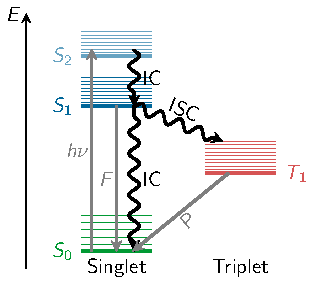
\includegraphics[scale=1.6]{img/jablonski/jablonski.pdf}
  \caption{Jab{\l}onski diagram showing the conceptual photophysical processes. Straight arrows show radiative processes: absorption ($h\nu$), fluorescence (F), and phosphorescence (P); wavy arrows show radiationless processes: internal conversion (IC) and intersystem crossing (ISC). }
  \label{fig:jablonski}
\end{figure}

The non-radiative IC and ISC process are fundamental concepts which play a decisive role in photochemistry and photobiology. IC processes are present in the excited-state dynamics of many organic and inorganic molecules, whose applications range from solar energy conversion to drug therapy. Even many, very small molecules, for example \ce{O2} and \ce{O3}, \ce{SO2}, \ce{NO2} and other nitrous oxides, show efficient IC, which has important consequences in atmospheric chemistry and the study of the environment and pollution. IC is also the first step of the biological process of visual perception, where the retinal moiety of rhodopsin absorbs a photon and non-radiatively performs a torsion around one of the double bonds, changing the conformation of the protein and inducing a neural signal. Similarly, protection of the human body from the influence of UV light is achieved through very efficient IC in DNA, proteins and melanins. Ultrafast IC to the electronic ground state allows quickly converting the excitation energy of the UV photons into nuclear kinetic energy, which is spread harmlessly as heat to the environment.

ISC processes are completely forbidden in the frame of the non-relativistic Schr\"odinger equation, but they become allowed when including spin-orbit couplings, a relativistic effect~\cite{Marian2012WCMS}. Spin-orbit coupling depends on the nuclear charge and becomes stronger for heavy atoms, therefore it is typically known as a ''heavy atom'' effect. However, it has been recently recognized that even for molecules with only first- and second-row atoms, ISC might be relevant and can be competitive in time scales with IC. A small selection of the growing number of molecules where efficient ISC in a sub-ps time scale has been predicted are \ce{SO2}~\cite{Wilkinson2014JCP,Mai2014JCP_SO2,Leveque2014JCP_ISC}, benzene~\cite{Penfold2012JCP}, aromatic nitrocompounds~\cite{Vogt2013JPC} or DNA nucleobases and derivatives~\cite{Crespo-Hernandez2004CR, Richter2012JPCL, Martinez-Fernandez2012CC, Mai2013C, Reichardt2010CC}.

% dynamics simulations
Theoretical simulations can greatly contribute to understand non-radiative processes by following the nuclear motion on the excited-state potential energy surfaces (PES) in real time. These simulations are called excited-state dynamics simulations. 
Since the Born-Oppenheimer approximation is not applicable for this kind of dynamics, non-adiabatic effects need to be incorporated into the simulations.

The principal methodology to tackle excited-state dynamics simulations is to numerically integrate the time-dependent Schr\"odinger equation, which is usually called full quantum dynamics simulations (QD). Given accurate PESs, QD is able to reach or surpass experimental accuracy. However, the need of an ''a priori'' knowledge of the full multi-dimensional PES renders this type of simulations quickly unfeasible for more than few degrees of freedom. Several alternative methodologies are possible to alleviate this problem. One of the most popular ones is to use surface hopping non-adiabatic dynamics.

% surface hopping, advantages, history
Surface hopping was originally devised by Tully~\cite{Tully1971JCP} and greatly improved later by the ``fewest-switches criterion''\cite{Tully1990JCP} and it has been reviewed extensively since then, see e.g.~\cite{Barbatti2011WCMS,Doltsinis2006,Doltsinis2002JTCC}.
In surface hopping, the motion of the excited-state wavepacket is approximated by the motion of an ensemble of many independent, classical trajectories. Each trajectory is at every instant of time tied to one particular PES, and the nuclear motion is integrated using the gradient of this PES. However, non-adiabatic population transfer can lead to the switching of a trajectory from one PES to another PES. This switching (also called ``hopping'', which is the origin of the name ``surface hopping'') is based on a stochastic algorithm, taking into account the change of the electronic population from one time step to the next one.

The advantages of the surface hopping methodology and thus its popularity are well summarized in Ref.~\cite{Barbatti2011WCMS}:
\begin{itemize}
  \item The method is conceptually simple, since it is based on classical mechanics. The nuclear propagation is based on Newton's equations and can be performed in cartesian coordinates, avoiding any problems with curved coordinate systems as in QD.
  \item For the propagation of the trajectories only local information of the PESs is needed. This avoids the calculation of the full, multi-dimensional PES in advance, which is the main bottleneck of QD methods. In surface hopping dynamics, all degrees of freedom can be included in the simulation. Additionally, all necessary quantities can be calculated on-demand, usually called ``on-the-fly'' in this context.
  \item The independent trajectories can be trivially parallelized.
\end{itemize}
The strongest of these points of course is the fact that all degrees of freedom can be included easily in the calculations, allowing to describe large systems.
%like DNA nucleobases, transition metal complexes and even large DNA strands and solvated molecules (by means of QM/MM schemes).
One should note, however, that surface hopping methods in the standard formulation~\cite{Tully1971JCP, Tully1990JCP} -- due to  the classical nature of the trajectories -- do not allow to treat some purely quantum-mechanical effects like tunneling, (tunneling for selected degrees of freedom is possible \cite{Hammes-Schiffer1994JCP}). Additionally, quantum coherence between the electronic states is usually described poorly, because of the independent-trajectory ansatz. This can be treated with some ad-hoc corrections, e.g., in \cite{Granucci2007JCP}.

% SHARC
In the original surface hopping method, only non-adiabatic couplings are considered, only allowing for population transfer between electronic states of the same multiplicity. 
The \sharc\ methodology is a generalization of standard surface hopping since it allows to include any type of coupling. Beyond non-adiabatic couplings (for IC), spin-orbit couplings (for ISC) or interactions of dipole moments with electric fields (to explicitly describe laser-induced processes) can be included.
A number of methodologies for surface hopping including one or the other type of potential couplings have been proposed in references~\cite{Thachuk1996JCP,Maiti2004JPCA,Jones2008JPCA,Mitric2009PRA,Granucci2012JCP,Curchod2013C,Cui2014JCP}, but \sharc\ can include all types of potential couplings on the same footing. 

The \sharc\ methodology is an extension to standard surface hopping which allows to include these kinds of couplings. The central idea of \sharc\ is to obtain a fully diagonal Hamiltonian, which is adiabatic with respect to all couplings. The diagonal Hamiltonian is obtained by unitary transformation of the Hamiltonian including all couplings. Surface hopping is conducted on the transformed electronic states.
This has a number of advantages over the standard surface hopping methodology, where no diagonalization is performed:
\begin{itemize}
  \item Potential couplings (like spin-orbit couplings and laser-dipole couplings) are usually delocalized. Surface hopping, however, rests on the assumption that the couplings are localized and hence surface hops only occur in the small region where the couplings are large. Within \sharc, by transforming away the potential couplings, additional terms of non-adiabatic (kinetic) couplings arise, which are localized. 
  \item The potential couplings have an influence on the gradients acting on the nuclei. To a good approximation, within \sharc\ it is possible to include this influence in the dynamics.
  \item When including spin-orbit couplings for states of higher multiplicity, diagonalization solves the problem of rotational invariance of the multiplet components (see~\cite{Granucci2012JCP}). 
\end{itemize}

The \sharc\ suite of programs is an implementation of the \sharc\ method. Besides the core dynamics code, it comes with a number of tools aiding in the setup, maintenance and analysis of the trajectories. 

\section{Capabilities}

The main features of the \sharc\ suite are:
\begin{itemize}
  \item Non-adiabatic dynamics based on the surface hopping methodology able to describe internal conversion and intersystem crossing with any number of states (singlets, doublets, triplets, or higher multiplicities).
  \item Algorithms for stable wavefunction propagation in the presence of very small or very large couplings.
  \item Inclusion of interactions with laser fields in the long-wavelength limit. The derivatives of the dipole moments can be included in strong-field applications.
  \item Propagation using either non-adiabatic couplings vectors $\langle\alpha|\frac{\partial}{\partial \mathbf{R}}|\beta\rangle$, time-derivative couplings $\langle\alpha|\frac{\partial}{\partial t}|\beta\rangle$ or wavefunction overlaps $\langle\alpha(t_0)|\beta(t)\rangle$ (via the local diabatization procedure \cite{Granucci2007JCP}).
  \item Gradients including the effects of spin-orbit couplings (with the approximation that the diabatic spin-orbit couplings are slowly varying).
  \item Energy-difference-based partial coupling approximation to speed up calculations \cite{Pittner2009CP}.
  \item Energy-based decoherence correction \cite{Granucci2007JCP}.
  \item Flexible interface to quantum chemistry programs. Existing interfaces to \textsc{Molpro} 2010 and 2012, \textsc{Molcas} 7.8 and 8.0, and to \textsc{Columbus 7.0} (only if interfaced to \textsc{Molcas}). An interface to implement dynamics based on analytical expressions is also available.
  \item Calculation of Dyson norms for single-photon ionization spectra through the \textsc{Columbus} interface.
  \item Suite of auxiliary Python scripts for all steps of the setup procedure and for various analysis tasks.
  \item Comprehensive tutorial.
\end{itemize}

%The following features are planned for future versions:
%\begin{itemize}
%  \item QM/MM calculations.
%  \item Dynamics in the Floquet picture.
%  \item Description of ionization processes by more advanced methods than Dyson norms.
%\end{itemize}

\section{References}

The following references should be cited when using the \sharc\ suite:
{
\newcommand{\enquote}[1]{``#1''}
\begin{shaded}
  % \begin{itemize}
  %   \item \cite{Mai2014WCMS} \bibentry{Mai2014WCMS}
  % \end{itemize}
  \begin{itemize}
    \item \cite{Richter2011JCTC} \bibentry{Richter2011JCTC}.
    \item \cite{Mai2014SHARC} \bibentry{Mai2014SHARC}.
  \end{itemize}
\end{shaded}
}

Further details can be found in the following references:

The theoretical background of \sharc\ is described in Refs.~\cite{Richter2011JCTC, Richter2012JCTC_erratum, Bajo2011JPCA, Marquetand2011FD}.

Applications of the \sharc\ code can be found in Refs.~\cite{Richter2012JPCL, Mai2013C, Mai2014TCC, Mai2014JCP_SO2, Gonzalez2014}.

Other features implemented in the \sharc\ suite are described in the following references:
\begin{itemize}
  \item Energy-based decoherence correction: \cite{Granucci2007JCP}.
  \item Local diabatization and wavefunction overlap calculation: \cite{Granucci2001JCP, Pittner2009CP, Plasser2012JCP}.
  \item Sampling of initial conditions from a quantum-mechanical harmonic Wigner distribution: \cite{Dahl1988JCP, Schinke1995}.
  \item Excited state selection for initial condition generation: \cite{Barbatti2011}.
  \item Calculation of ring puckering parameters and their classification: \cite{Cremer1975JACS, Boeyens1976JCMS}.
\end{itemize}

The quantum chemistry programs to which interfaces with \sharc\ exist are described in the following sources:
\begin{itemize}
  \item \textsc{Columbus}: \cite{Lischka2011WCMS, Lischka2012, Yabushita1999JPCA, Mai2014JCP_reindex},
  \item \textsc{Molpro}: \cite{Werner2012WCMS, Werner2012},
  \item \textsc{Molcas}: \cite{Karlstrom2003CMS, Aquilante2010JCC}.
\end{itemize}

\section{Authors}

The current version of the \sharc\ suite has been programmed by Sebastian Mai and Martin Richter of the AG Gonz\'alez of the Institute of Theoretical Chemistry of the University of Vienna with contributions from Jes\'us Gonz\'alez-V\'azquez, Philipp Marquetand, Matthias Ruckenbauer, Markus Oppel and Leticia Gonz\'alez.

\section{Suggestions and Bug Reports}

\begin{shaded}
Bug reports and suggestions for possible features can be submitted to \href{mailto:sharc@univie.ac.at}{sharc@univie.ac.at}.
\end{shaded}

\section{Notation in this Manual}

\paragraph{Names of programs}

The \sharc\ suite consists of Fortran90 programs as well as Python and Shell scripts. The executable Fortran90 programs are denoted by the extension \ttt{.x}, the Python scripts have the extension \ttt{.py} and the Shell scripts \ttt{.sh}. Within this manual, all program names are given in \ttt{bold monospaced font}.

\tthdump{
\paragraph{Shaded Sections}

Important sections are given in blue boxes like the following one:
\begin{shaded}
Important sections are given in blue boxes like this one.
\end{shaded}

On the other hand, examples of input files and command lines are marked like this:
\begin{example}
  \tt user@host$>$ example example.dat
\end{example}
}



% ========================================================================================================= %
% ========================================================================================================= %
% ========================================================================================================= %

\chapter{Installation}

\section{How To Obtain}

\sharc\ can be obtained from the \sharc\ homepage \href{http://sharc-md.org}{www.sharc-md.org}. In the Download section, register with your e-mail adress and affiliation. You will receive a download link to the stated e-mail adress. Clicking on the link in the email will download the archive file containing the \sharc\ package. Note that the link is active only for 24 h and the number of downloads is limited.

Note that you must accept the Terms of Use given in the following section in order to download \sharc.

\section{Terms of Use}

\newcounter{licenseparacount}
\newcommand{\licensepara}[1]{\vspace{\bigskipamount}\addtocounter{licenseparacount}{1}\textbf{\thelicenseparacount.\quad#1}\newline}
{
\definecolor{shadecolor}{HTML}{BBDDFF}
\begin{shaded}
\licensepara{Recitals}

The University of Vienna (in following the ``University''), whose principal address is at Universit\"ats\-ring 1, 1010 Vienna, Austria, developed the Software ``SHARC: Surface Hopping with Arbitrary Couplings. A program suite to study the excited-state dynamics of molecules'' (in the following the ``Software'').

The Software is not to be used for commercial purposes. Our Software provided on the relevant website is solely to be used for research, teaching and demonstration purposes and is free of any charge. The user of the Software is required to have the appropriate knowledge and know-how to use the Software (in the following the ``User''). Any User should seek further guidance and make independent enquiries before relying on the Software.

\licensepara{Research, Teaching and Demonstration Purposes, Content and Liability}

The Software on this website is based on scientific work and is solely to be used for research, teaching and demonstration purposes. The University, its organs, associated companies, employees and representatives do not warrant, represent or guarantee the functionality of the Software whatsoever. 

The use of the Software is at your own risk and your own responsibility. The University, its organs, associated companies, employees and representatives do not assume any liability for the use the Software including its results. The University does not warrant, represent or guarantee any quality or performance of the Software and shall not be responsible for including but not limited to

\begin{itemize}
  \item any contents of the Software in any kind;
  \item any intermediate or permanent amendments of the Software of any kind;
  \item any damages of any kind arising out of or in connection with the use of the Software (including without limitation damages for any consequential loss or loss of business opportunities or projects, or loss of profits) including, but not limited to, data theft or data loss;
  \item any errors, faults, incompleteness, inaccuracy, inadequacy or unsuitability or incorrectness of the provided Software or its results;
  \item any personal damages or damages to property due to the use of the Software;
  \item any damages of computers, any viruses or Trojans or similar which were transferred or conveyed by the Software;
  \item any defaults or incompleteness of the Software including any loss or damages of any kind due to or arising out of the use of the Software provided on the website of the University;
  \item any damages caused by third persons or subcontractors.
\end{itemize}

Hence, the University explicitly reserves the right to amend, supplement, delete or remove the Software, partially or as a whole, at any time and without prior notice.

The University explicitly refrains from and does not assume any liability whatsoever for any products or services offered or advertised by third persons via the provided Software.

\licensepara{Acknowledgements}

The User shall acknowledge the authors or originators and use of the Software in the publication of any results achieved through use of the Software in the form of including the following references:

\begin{itemize}
  \item S. Mai, M. Richter, M. Ruckenbauer, M. Oppel, P. Marquetand, L. Gonz\'alez: ``SHARC: Surface Hopping Including Arbitrary Couplings - Program Package for Non-Adiabatic Dynamics''. www.sharc-md.org (2014).
  \item M. Richter, P. Marquetand, J. Gonz\'alez-V\'azquez, I. Sola, L. Gonz\'alez: ``SHARC: ab Initio Molecular Dynamics with Surface Hopping in the Adiabatic Representation Including Arbitrary Couplings''. J. Chem. Theory Comput., 7, 1253-1258 (2011).
\end{itemize}

The User shall reproduce a copyright notice on every copy of the Software including partial copies and on any accompanying manuals and documentation in the form ``Copyright \copyright\ 2014 University of Vienna. All rights reserved.'' Trademark and other proprietary notices must also be reproduced but the User has no longer the right to use the name, arms, trademark, logo or other designation of the University of Vienna.

\licensepara{Intellectual Property}

The contents of this Software are exclusively governed and construed by Austrian intellectual property laws. Any copying, editing, distribution or use of the contents require the prior consent of the respective authors or originators which is not granted or deemed to be granted without the prior written consent as described above.

If and to the extent the User amends, edits or otherwise supplements the Software with own information or other information of third persons, the User shall be deemed as the new operator of the Software. Consequently, the User expressly assumes any and all liability in connection with the Software.

\licensepara{Indemnity}

The User is irrevocably obliged to indemnify the University, its employees, its organs, its associated companies and representatives for any damages in particular claims and damage claims including legal cost for
\begin{itemize}
  \item any use of the Software by the User;
  \item any violation or infringement of this terms of use partially or in whole;
  \item any violation of rights of third persons in particular of intellectual property rights or personality rights of publicity or
  \item any claims of third persons due to the use of the Software.
\end{itemize}

This obligation of the User to indemnify shall not impede any other provision of this disclaimer described herein and shall remain in force and effect after the User has ceased to use the Software.

If and to the extent third persons assert any claims against the University due to or arising out of the use by any User, such User shall be obliged to indemnify and hold harmless the University for any damages asserted against the University.

\licensepara{Data Protection}

The User explicitly acknowledges that the University uses services of third party suppliers (e.g. Google Analytics etc.) and consents to the use of its data by the third party supplier. Further, the User consents to the use of the respective IP address of the User or similar by third persons (e.g. for statistical use). The University shall be entitled to provide third persons with such data for statistical purposes. If personal data of Users is provided to or used by third persons, the University shall not be deemed as a sponsor pursuant to the Austrian Data Protection Act 2000.

\licensepara{Final Provisions}

The Software was developed in Austria and is applicable through a server located in Austria. Any and all interpretation of the content of the Software, any claims with regards to the Software and any disputes in connection with the Software shall be governed by Austrian law excluding any applicable collision provisions. Exclusive place of jurisdiction shall be Vienna, Austria.

\end{shaded}
}


\section{Installation}

In order to install and run \sharc\ under Linux (Windows and OS X are currently not supported), you need the following:
\begin{itemize}
  \item A Fortran90 compiler (This release is tested against \href{https://gcc.gnu.org/fortran/}{GNU Fortran} 4.4.7 and \href{https://software.intel.com/en-us/fortran-compilers}{Intel Fortran} 15.0).
  \item The \href{http://www.netlib.org/blas/}{BLAS}, \href{http://www.netlib.org/lapack/}{LAPACK} and \href{http://http://www.fftw.org/}{FFTW3} libraries.
  \item \href{https://www.python.org/downloads/release/python-278/}{Python 2} (This release is tested against Python 2.6.6 and 2.7.3).
\end{itemize}

The source code of the  \sharc\ suite is distributed as a tar archive file. In order to install it, first extract the content of the archive to a suitable directory:
\begin{example}
\verb|tar -xzvf sharc.tgz|
\end{example}
This should create a new directory called \ttt{sharc/} which contains all the necessary subdirectories and files. 

To compile the Fortran90 programs of the \sharc\ suite, go to the \ttt{source/} directory.
\begin{example}
\verb|cd source/|
\end{example}
and edit the \ttt{Makefile} by adjusting the \ttt{F90} variable to point to the Fortran compiler of your choice. 
Issuing the command:
\begin{example}
\verb|make|
\end{example}
will compile the source and create all the binaries.
\begin{example}
\verb|make install|
\end{example}
will copy the binary files into the \ttt{sharc/bin/} directory of the 
\sharc\ distribution, which already contains all the python scripts which
come with \sharc.
In figure~\ref{fig:installation} the directory structure of the complete \sharc\ directory is shown.

\begin{figure}[h!]
  \centering
  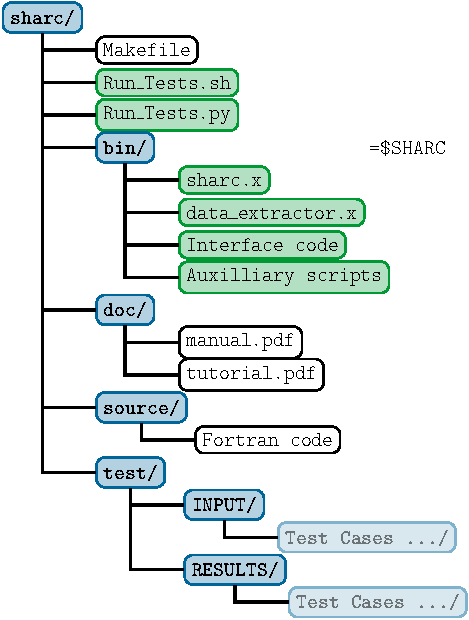
\includegraphics[scale=1]{img/dirs_SHARC/dirs_SHARC.pdf}
  \caption{Directory tree containing a complete \sharc\ installation.}
  \label{fig:installation}
\end{figure}

In order to use the \sharc\ suite, set the environment variable \ttt{\$SHARC} to the \ttt{bin/} directory of the \sharc\ installation. This ensures that all programs of the \sharc\ suite find the other executables and all calls are successful. For example, if you have unpacked \sharc into your home directory, 
just set: 
\begin{example}
\verb|export SHARC=~/sharc/bin|\quad (for bourne shell users)
\end{example}
or
\begin{example}
\verb|setenv SHARC $HOME/sharc/bin|\quad (for c-shell type users)
\end{example}
Note that it is advisable to put this line into your shell's login
scripts.

\subsection{Libraries}

\sharc\ requires the BLAS, LAPACK and FFTW3 libraries. During the installation, it might be necessary to alter the \ttt{LDFLAGS} string in the \ttt{Makefile}, depending on where the relevant libraries are located on your system. In this way, it is for example possible to use vendor-provided libraries like the \href{https://software.intel.com/en-us/intel-mkl}{Intel MKL}. For more details see the \ttt{INSTALL} file which is included in the \sharc\ distribution.

\subsection{Test Suite}

After the installation, it is advisable to first execute the test suite of \sharc, which will test the fundamental functionality of SHARC.
Change to an empty directory and execute
\begin{example}
\verb|$SHARC/tests.py|
\end{example}
The interactive script will first verify the Python installation (no message will appear if the Python installation is fine). Subsequently, the script prompts the user to enter which tests should be executed. Their is at least one test for each of the auxiliary scripts and interfaces. Tests whose names start with \ttt{scripts\_} test the functionality of the auxiliary programs in the \sharc\ suite. Tests whose names start with \ttt{Analytical\_}, \ttt{COLUMBUS\_}, \ttt{MOLCAS\_} or \ttt{MOLPRO\_} run short trajectories, testing whether the main dynamics code, the interfaces and the quantum chemistry programs work together correctly.

If the installation was successful and Python is installed correctly, the tests named \ttt{scripts\_<NAME>} and \ttt{Analytical\_overlap} should execute without error. 

The test calculations involving the quantum chemistry programs (\textsc{Columbus}, \textsc{Molcas}, \textsc{Molpro}) can be used to check that \sharc\ can correctly call these programs and that they are installed correctly.

If any of the tests show differences between output and reference output, it is advisable to check the respective files. Note that small differences in the output can already occur when using a different version of the quantum chemistry programs, and that these small differences can add up during the simulations.

\subsection{Additional Programs}

For full functionality of the \sharc\ suite, several additional programs are recommended:
\begin{itemize}
  \item The Python package \href{http://www.numpy.org/}{\textsc{NumPy}}.
  \item The \href{http://www.gnuplot.info/}{\textsc{Gnuplot}} plotting software.
  \item A program for molecular visualization, able to read files in the xyz file format (e.g.\ \href{http://www.cmbi.ru.nl/molden/molden.html}{\textsc{Molden}}, \href{http://gabedit.sourceforge.net/}{\textsc{Gabedit}}, \href{http://molekel.cscs.ch/wiki/pmwiki.php}{\textsc{Molekel}} or \href{http://www.ks.uiuc.edu/Research/vmd/}{VMD})
\end{itemize}

Optimally, within your Python installation the \textsc{NumPy} package (which provides many numerical methods, e.g., matrix diagonalization) should be available. If \textsc{NumPy} is not available, the \sharc\ suite is still functional, and the affected scripts will fall back to use a small Fortran code (front-end for LAPACK) within the \sharc\ package. Since in the Python scripts no large-scale matrix calculations are carried out, there should be no significant performance loss if \textsc{NumPy} is not available.

\textsc{Gnuplot} is not strictly necessary, since all output files could be plotted using other plotting programs. However, a number of scripts from the \sharc\ suite automatically generate \textsc{Gnuplot} scripts after data processing, allowing to quickly plot the output files.

% Molecular visualization software ..

\subsection{Quantum Chemistry Programs}

Even though \sharc\ comes with an interface for analytical potentials (and hence can be used without any quantum chemistry program), the main application of \sharc\ is certainly on-the-fly ab initio dynamics. Hence, one of the following interfaced quantum chemistry programs is necessary:
\begin{itemize}
  \item \href{http://www.molpro.net/}{\textsc{Molpro}} (this release was checked against \textsc{Molpro} 2010 and 2012).
  \item \href{http://http://molcas.org/}{\textsc{Molcas}} (this release was checked against \textsc{Molcas} 7.8 and 8.0).
  \begin{itemize}
    \item \href{http://www.univie.ac.at/columbus/docs_COL70/documentation_main.html}{\textsc{Columbus} 7}, interfaced to \href{http://http://molcas.org/}{\textsc{Molcas}}, for correlated multi-reference wavefunctions. 
%     \item \href{http://dasher.wustl.edu/tinker/}{Tinker}, interfaced to \textsc{Molcas} 7.8 or 8.0 for QM/MM dynamics.
  \end{itemize}
\end{itemize}

See the relevant sections in chapter~\ref{chap:interfaces} for a description of the quantum chemical methods available with each of these programs.

% ========================================================================================================= %
% ========================================================================================================= %
% ========================================================================================================= %

\chapter{Execution}

The \sharc\ suite consists of the main dynamics code \ttt{sharc.x} and a number of auxiliary programs, like setup scripts and analyse tools. Additionally, the suite comes with interfaces to suitable quantum chemistry software, e.g.\ \textsc{Molpro}, \textsc{Molcas} or \textsc{Columbus}. 

In the following, first it is explained how to run a single trajectory by setting up all necessary input for the dynamics code \ttt{sharc.x} manually. Afterwards, the usage of the auxiliary scripts is explained. Detailed infos on the \sharc\ input files is given in chapter~\ref{chap:input} and on the auxiliary scripts in chapter~\ref{chap:aux}. The interfaces are described in chapter~\ref{chap:interfaces}.

\section{Running a single trajectory}

\subsection{Input files}

\sharc\ requires a number of input files, which contain the settings for the dynamics simulation (\ttt{input}), the initial geometry (\ttt{geom}), the initial velocity (\ttt{veloc}), the initial coefficients (\ttt{coeff}) and the laser field (\ttt{laser}). Only the first two (\ttt{input}, \ttt{geom}) are mandatory, the others are optional. The necessary files are shown in figure~\ref{fig:dir_traj}. 
The content of the main input file is explained in detail in section~\ref{sec:inputfile}, the geometry file is specified in section~\ref{sec:geomfile}. The specifications of the velocity, coefficient and laser files are given in sections~\ref{sec:velocfile}, \ref{sec:coefffile} and \ref{sec:laserfile}, respectively.

\begin{figure}[h!]
  \centering
  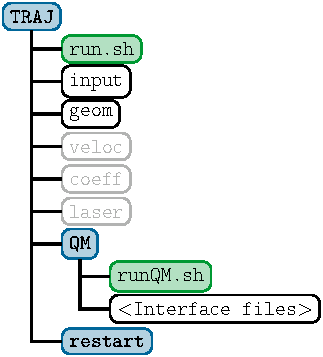
\includegraphics[scale=1]{img/dir_traj/dir_traj.pdf}
  \caption{Input files for a \sharc\ dynamics simulation. Directories are in blue, executable scripts in green, regular files in white and optional files in grey.}
  \label{fig:dir_traj}
\end{figure}

Additionally, the directory \ttt{QM/} and the script \ttt{QM/runQM.sh} need to be present, since the on-the-fly ab initio calculations are implemented through these files. The script \ttt{QM/runQM.sh} is called each time \sharc\ performs an on-the-fly calculation of electronic properties (usually by a quantum chemistry program). In order to do so, \sharc\ first writes the request for the calculation to \ttt{QM/QM.in}, then calls \ttt{QM/runQM.sh}, waits for the script to finish and then reads the requested quantities from \ttt{QM/QM.out}. The script \ttt{QM/runQM.sh} is fully responsible to generate the requested results from the provided input. 
In virtually all cases, this task is handled by the \sharc-quantum chemistry interfaces (see chapter~\ref{chap:interfaces}), so that the script \ttt{QM/runQM.sh} has a particularly simple form:
\begin{example}
\verb|cd QM/|

\verb|$SHARC/<INTERFACE> QM.in |
\end{example}
with the corresponding interface name given. Note that the interfaces in all cases need additional input files, which must be present in \ttt{QM/}. Those input files contain the specifications for the quantum chemistry information, e.g., basis set, active and reference space, memory settings, path to the quantum chemistry program, path to scratch directories; or for \ttt{SHARC\_Analytical.py}, the expressions for the analytical potentials. For each interface, the input files are slightly different. See sections~\ref{sec:int:molpro}, \ref{sec:int:molcas}, \ref{sec:int:columbus} or \ref{sec:int:analytical} for the necessary information.

\subsection{Running the dynamics code}

Given the necessary input files, \sharc\ can be started by executing
\begin{example}
\verb|user@host> $SHARC/sharc.x input|
\end{example}
Note that besides the input file, at least the geometry file needs to be present (see in the input section for details).

\subsection{Output files}

Figure~\ref{fig:dir_traj_after} shows the content of a trajectory directory after the execution of \sharc. There will be six new files. These files are \ttt{output.log}, \ttt{output.lis}, \ttt{output.dat} and \ttt{output.xyz}, as well as \ttt{restart.ctrl} and \ttt{restart.traj}.

The file \ttt{output.log} contains mainly a listing of the chosen options and the resulting dynamics settings. At higher print levels, the log file contains also information per timestep (useful for debugging). \ttt{output.lis} contains a table with one line per timestep, giving active states, energies and expectation values. \ttt{output.dat} contains a list of all important matrices and vectors at each timestep. This information can be extracted with \ttt{data\_extractor.x} to yield plottable table files. \ttt{output.xyz} contains the geometries of all timesteps (the comments to each geometry give the active state).
For details about the content of the output files, see chapter~\ref{chap:output}.

The restart files contain the full state of a trajectory and its control variables from the last successful timestep. These files are needed in order to restart a trajectory at this timestep (either because the calculation failed, or in order to extend the simulation time beyond the original maximum simulation time). 

\begin{figure}[h!]
  \centering
  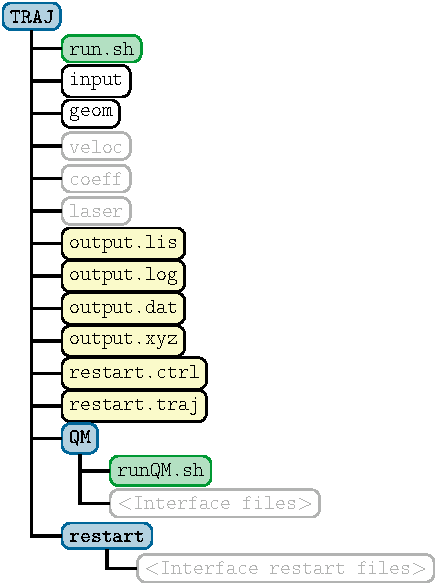
\includegraphics[scale=1]{img/dir_traj/dir_traj_after.pdf}
  \caption{Files of a \sharc\ dynamics simulation after running. Directories are in blue, executable scripts in green, regular files in white and optional files in grey. Output files are in yellow.}
  \label{fig:dir_traj_after}
\end{figure}

\section{Typical workflow for an ensemble of trajectories}

Usually, one is not interested in running only a single trajectory, since a single trajectory cannot reproduce the branching of a wavepacket into different reaction channels. In order to do so, within surface hopping an ensemble of independent trajectories is employed. 

When dealing with a (possibly large) ensemble of trajectories, setup and analysis need to be automatized. Hence, the \sharc\ suite contains a number of scripts fulfilling different tasks in the usual workflow of setting up ensembles of trajectories.
The typical workflow is given schematically in figure~\ref{fig:workflow}.

\begin{figure}[h!]
  \centering
  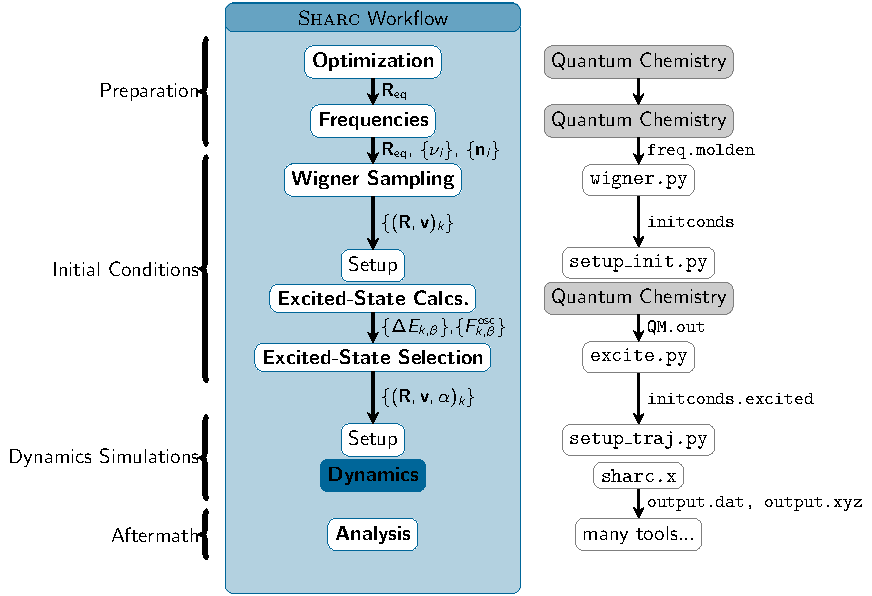
\includegraphics[scale=1]{img/workflow/prepare.pdf}
  \caption{Typical workflow for conducting excited-state dynamics simulations with \sharc.}
  \label{fig:workflow}
\end{figure}

\subsection{Initial condition generation}

In the typical workflow, the user will first create a set of suitable initial conditions. In the context of the \sharc\ package, an initial condition is a set of an initial geometry, initial velocity, initial occupied state and initial wavefunction coefficients. 
Many such sets are needed in order to setup physically sound dynamics simulations.

\paragraph{Generation of initial geometries and velocities}

Currently, within the \sharc\ suite, initial geometries and velocities can be generated based on a quantum harmonic oscillator Wigner distribution. The theoretical background is given in section~\ref{met:wigner}. The calculation is performed by \ttt{wigner.py}, which is explained in section~\ref{sec:wigner.py}. 

As given in figure~\ref{fig:workflow}, \ttt{wigner.py} needs as input the result of a frequency calculation in \textsc{Molden} format. The calculation can be performed by any quantum chemistry program and any method the user sees fit. 
\ttt{wigner.py} produces the file \ttt{initconds}, which contains a list of initial conditions ready for further processing.

\paragraph{Generation of initial coefficients and states}

In the second preparation step, for each of the sampled initial geometries it has to be decided which excited state should be the initial one. In simple cases, the user may manually choose the initial excited state using \ttt{excite.py} (see~\ref{sec:excite.py}). Alternatively, the selection of initial states can be performed based on the excitation energies and oscillator strengths of the excited states at each initial geometry (\todo{this approximately simulates a delta-pulse excitation}). 

The latter option makes it necessary to carry out vertical excitation calculation before the selection of the initial states.
The calculations can be set up with \ttt{setup\_init.py} (see section~\ref{sec:setup_init.py}). This script prepares for each initial condition in the \ttt{initconds} file a directory with the necessary input to perform the calculation. The user should then execute the run script (\ttt{run.sh}) in each of the directories (either manually or through a batch queueing system).

After the vertical excitation calculations are completed, the vertical excitation energies and oscillator strengths of each calculation are collected by \ttt{excite.py} (see~\ref{sec:excite.py}). The same script then performs the selection of the initial electronic state for each initial geometry. The results are written to a new file, \ttt{initconds.excited}. This file contains all information needed to setup the ensemble. 

Additionally, \ttt{spectrum.py} (\ref{sec:spectrum.py}) can calculate absorption spectra based on the \ttt{initconds.excited} file. This may be useful to verify that the level of theory chosen is appropriate (e.g., by comparing to an experimental spectrum), or to choose a suitable excitation window for the determination of the initial state.

\subsection{Running the dynamics simulations}

Based on the initial conditions given in \ttt{initconds.excited}, the input for all trajectories in the ensemble can be setup by \ttt{setup\_traj.py} (see section~\ref{sec:setup_traj.py}). The script produces one directory for each trajectory, containing the input files for \sharc\ and the selected interface.

In order to run a particular trajectory, the user should execute the run script (\ttt{run.sh}) in the directory of the trajectory. Since those calculations can run between minutes and several weeks (depending on the level of theory used and the number of timesteps), it is advisable to submit the run scripts to a batch queueing system. 

The progress of the simulations can be monitored most conveniently in the \ttt{output.lis} files. If the calculations are running in some temporary directory, the output files can be copied to the local directory (where they were setup) with the \ttt{scp} wrapper \ttt{retrieve.sh} (see \ref{sec:retrieve}). This allows to perform ensemble analysis while the trajectories are still running.

If a trajectory fails, the temporary directory where the calculation is running is not deleted. The file \ttt{README} will be created in the trajectory's directory, giving the time of the failure and the location of the temporary data, so that the case can be investigated. 

\subsection{Analysis of the dynamics results}

Each trajectory can be analyzed independently by inspecting the output files (see chapter~\ref{chap:output}). Most importantly, calling \ttt{data\_extractor.x} (\ref{sec:data_extractor.x}) on the \ttt{output.dat} file of a trajectory creates a number of formatted files which can be plotted with the help of \ttt{make\_gnuscript.py} (\ref{sec:make_gnuscript.py}) and \textsc{Gnuplot}.
The nuclear geometries in \ttt{output.xyz} file can be analyzed in terms of internal coordinates (bond lengths, angles, ring conformations, etc.) using \ttt{geo.py} (\ref{sec:geo.py}).

For the complete ensemble, the script \ttt{populations.py} (section~\ref{sec:populations.py} can calculate average excited-state populations. The script~\ttt{crossing.py} (\ref{sec:crossing.py}) can find and extract notable geometries, e.g., those geometries where a surface hop between two particular states occured.

\section{Auxilliary Programs and Scripts}

The following tables list the auxiliary programs in the \sharc\ suite. The rightmost column gives the section where the program is documented.

\subsection{Setup}

\begin{tabular}{>{\tt}lp{9.5cm}r}
  wigner.py             &Creates initial conditions from Wigner distribution.                   &\ref{sec:wigner.py}\\
  setup\_init.py        &Sets up initial vertical excitation calculations.                              &\ref{sec:setup_init.py}\\
  excite.py             &Generates excited state lists for initial conditions and selects initial states.                                            &\ref{sec:excite.py}\\
  setup\_traj.py        &Sets up the dynamics simulations based on the initial conditions.      &\ref{sec:setup_traj.py}\\
  laser.x               &Prepares files containing laser fields.                                &\ref{sec:laser.x}\\
  molpro\_input.py      &Prepares \textsc{Molpro} input files for common jobs.                  &\ref{sec:molpro_input.py}\\
  molcas\_input.py      &Prepares template files for the \textsc{Molcas} interface.             &\ref{sec:molcas_input.py}\\
  diagonalizer.x        &Helper program for \ttt{excite.py}. Only required if \textsc{NumPy} is not available.            &\ref{sec:diagonalizer.x}\\
\end{tabular}

\subsection{Analysis}

\begin{tabular}{>{\tt}lp{9.5cm}r}
  spectrum.py           &Generates absorption spectra from initial conditions files.            &\ref{sec:spectrum.py}\\
  retrieve.sh           &\ttt{scp} wrapper to retrieve dynamics output during the simulation.   &\ref{sec:retrieve}\\
  data\_extractor.x     &Extracts plottable results from the \sharc\ output data file.          &\ref{sec:data_extractor.x}\\
  make\_gnuscript.py    &Creates gnuplot scripts for a given number of states.                  &\ref{sec:make_gnuscript.py}\\
  populations.py        &Calculates ensemble populations.                                       &\ref{sec:populations.py}\\
  crossing.py           &Extracts specific geometries from ensembles.                                          &\ref{sec:crossing.py}\\
  geo.py                &Calculates internal coordinates from xyz files.              &\ref{sec:geo.py}\\
\end{tabular}

\subsection{Interfaces}

\begin{tabular}{>{\tt}lp{9.5cm}r}
  SHARC\_MOLPRO.py      &Allows for the calculation of SOC, gradients, non-adiabatic couplings, time derivatives, overlaps, dipole moments and angular momentum expectation values at the CASSCF level of theory. Symmetry or RASSCF are not supported. Only segmented basis sets are possible.   &\ref{sec:int:molpro}\\
  SHARC\_MOLCAS.py      &Allows for the calculation of SOC, gradients, overlaps and dipole moments at the CASSCF and RASSCF level of theory. Symmetry is not supported.   &\ref{sec:int:molcas}\\
  SHARC\_COLUMBUS.py    &Allows for the calculation of SOC, gradients, overlaps, dipole moments and Dyson norms at the CASSCF, RASSCF, MRCISD and LRT-MRAQCC levels of theory. Symmetry is not supported. Only works with the \textsc{Columbus}-\textsc{Molcas} interface.                  &\ref{sec:int:columbus}\\
  SHARC\_Analytical.py  &Allows to calculate SOC, gradients, overlaps, dipole moments and dipole moment gradients based on analytical expressions of diabatic matrix elements. Works only with cartesian coordinates.       &\ref{sec:int:analytical}\\
\end{tabular}



% ========================================================================================================= %
% ========================================================================================================= %
% ========================================================================================================= %

\chapter{Input files}\label{chap:input}

In this chapter, the format of all \sharc\ input files are presented. Those are the main input file (here called \ttt{input}), the geometry file, the velocity file, the coefficients file and the laser file. Only the first two are mandatory, the others are optional input files. All input files are ASCII text files.

% ========================================================================================================= %

\section{Main input file}\label{sec:inputfile}

This section presents the format and all input keywords for the main \sharc\ input. Note that when using \ttt{setup\_traj.py}, full knowledge of the \sharc\ input keywords is not required.

\subsection{General remarks}

The input file has a relatively flexible structure. With very few exceptions, each single line is independent. An input line starts with a keyword, followed optionally by a number of arguments to this keyword. Example:

\begin{example}
  \verb|stepsize 0.5|
\end{example}

Here, \ttt{stepsize} is the keyword, referring to the size of the timesteps for the nuclear motion in the dynamics. \ttt{0.5} gives the size of this timestep, in this example 0.5~fs.

A number of keywords have no arguments and act as simple switches (e.g., \ttt{restart}, \ttt{gradcorrect}, \ttt{grad\_select}, \ttt{nac\_select}, \ttt{ionization}, \ttt{track\_phase}, \ttt{dipole\_gradient}). Those keywords can be prefixed with \ttt{no} to explicitly deactivate the option (e.g., \ttt{norestart} deactivates restarts).

In each line a trailing comment can be added in the input file, by using the special character \ttt{\#}. Everything after \ttt{\#} is ignored by the input parser of \sharc. The input file also can contain arbitrary blank lines and lines containing only comments. All input is case-insensitive.

The input file is read by \sharc\ by subsequently searching the file for all known keywords. Hence, unknown or misspelled keywords are ignored. Also, the order of the keywords is completely arbitray. Note however, that if a keyword is repeated in the input only the \textit{first} instance is used by the program. 

\subsection{Input keywords}

In Table~\ref{tab:input}, all input keywords for the \sharc\ input file are listed.

\clearpage
{
%%tth: \newcommand{\DEFAULT}[1]{\textbf{\textcolor{PineGreen}{#1}}}
\tthdump{
  \newcommand{\DEFAULT}[1]{\textbf{\textcolor{G}{#1}}}
}
\begin{longtable}{|>{\tt}l|l|p{7cm}|}
  \caption{Input keywords. The first column gives the name of the keyword, the second lists possible arguments and the third line provides an explanation. Defaults are marked like \DEFAULT{this}. \$$n$ denotes the $n$-th argument to the keyword.}  \label{tab:input}\\

% ========================================

    \hline
    \rmfamily Keyword     &Arguments    &Explanation\\
    \hline
  \endfirsthead

% ========================================

\tthdump{
    \multicolumn{3}{c}{{\bfseries \tablename\ \thetable{} \mdseries-- Continued from previous page}} \\
    \hline
    \rmfamily Keyword     &Arguments    &Explanation\\
    \hline
  \endhead
}

% ========================================

\tthdump{
    \hline 
    \multicolumn{3}{r}{{Continued on next page}} \\ 
%     \hline
  \endfoot
}
  
% =======================================

\tthdump{
    \hline
  \endlastfoot
}

% ========================================

  printlevel            &\textbf{integer}                    &Controls the verbosity of the log file.\\
                        &\$1=0                               &{\footnotesize Log file is empty}\\
                        &\$1=1                               &{\footnotesize + List of internal steps}\\
                        &\$1\DEFAULT{=2}                     &{\footnotesize + Input parsing information}\\
                        &\$1=3                               &{\footnotesize + Some information per timestep}\\
                        &\$1=4                               &{\footnotesize + More information per timestep}\\
                        &\$1=5                               &{\footnotesize + Much information per timestep}\\
  \hline
  restart               &                                    &Dynamics is resumed from restart files.\\
  \DEFAULT{norestart}    &                                    &Dynamics is initialized from input files.\\
                        &                                    &{\footnotesize \ttt{norestart} takes precedence.}\\
  \hline
  nstates               &list of \textbf{integer}s           &Number of states per multiplicity.\\
                        &\$1 (\DEFAULT{1})                   &{\footnotesize Number of singlet states}\\
                        &\$2 (\DEFAULT{0})                   &{\footnotesize Number of doublet states}\\
                        &\$3 (\DEFAULT{0})                   &{\footnotesize Number of triplet states}\\
                        &\$\dots (\DEFAULT{0})               &{\footnotesize Number of states of higher multiplicities}\\
  \hline
  actstates             &list of \textbf{integer}s           &Number of active states per multiplicity.\\
                        &\DEFAULT{same as \ttt{nstates}}     &{\footnotesize By default, all states are active.}\\
  \hline
  state                 &\textbf{integer}, \textbf{string}   &Specifies the initial state (no default; \sharc\ exits if \ttt{state} is missing).\\
                        &\$1                                 &{\footnotesize Initial state.}\\
                        &\$2=MCH                             &{\footnotesize Initial state and coefficients are given in MCH representation.}\\
                        &\$2=diag                            &{\footnotesize Initial state and coefficients are given in diagonal representation.}\\
  \hline
  coeff                 &\textbf{string}                     &Sets the wavefunction coefficients.\\
                        &\$1\DEFAULT{=auto}                  &{\footnotesize Initial coefficient are determined automatically from initial state.}\\
                        &\$1=external                        &{\footnotesize Initial coefficients are read from file.}\\
  \hline
  coefffile             &\textbf{quoted string}              &File containing the initial wavefunction coefficients.\\
                        &\DEFAULT{"coeff"}                   &\\
  \hline
  geomfile              &\textbf{quoted string}              &File name containing the initial geometry.\\
                        &\DEFAULT{"geom"}                    &\\
  \hline
  veloc                 &\textbf{string}                     &Sets the initial velocities.\\
                        &\$1\DEFAULT{=zero}                  &{\footnotesize Initial velocities are zero.}\\
                        &\$1=random \$2 \textbf{float}       &{\footnotesize Initial velocities are determined randomly with \$2 eV kinetic energy per atom.}\\
                        &\$1=external                        &{\footnotesize Initial velocities are read from file.}\\
  \hline
  velocfile             &\textbf{quoted string}              &File containing the initial velocities.\\
                        &\DEFAULT{"veloc"}                   &\\
  \hline
  laser                 &\textbf{string}                     &Sets the laser field.\\
                        &\$1\DEFAULT{=none}                  &{\footnotesize No laser field is applied.}\\
                        &\$1=internal                        &{\footnotesize Laser field is calculated at each timestep from internal function.}\\
                        &\$1=external                        &{\footnotesize Laser field for each timestep is read during initialization.}\\
  \hline
  laserfile             &\textbf{quoted string}              &File containing the laser field.\\
                        &\DEFAULT{"laser"}                   &\\
  \hline
  laserwidth            &\textbf{float}                      &Laser bandwidth used to detect induced hops.\\
                        &\DEFAULT{1.0 eV}                    &\\
  \hline
  stepsize              &\textbf{float}                      &Length of the nuclear dynamics timesteps in fs.\\
                        &\DEFAULT{0.5 fs}                    &\\
  \hline
  nsubsteps             &\textbf{integer}                    &Number of substeps for the integration of the electronic equation of motion.\\
                        &\DEFAULT{25}                        &\\
  \hline
  nsteps                &\textbf{integer}                    &Number of simulation steps.\\
                        &\DEFAULT{3}                         &\\
  \hline
  tmax                  &\textbf{float}                      &Total length of the simulation in fs.\\
                        &                                    &{\footnotesize No effect if \ttt{nsteps} is present.}\\
  \hline
  killafter             &\textbf{float}                      &Terminates the trajectory after \$1 fs in the lowest state. If \$1$<$0, trajectories are never killed.\\
                        &\DEFAULT{-1}                        &\\
  \hline
  surf                  &\textbf{string}                     &Chooses the potential energy surfaces used in surface hopping.\\
                        &\$1\DEFAULT{=sharc}                 &{\footnotesize Uses the diagonal potentials.}\\
                        &\$1=fish                            &{\footnotesize Uses the MCH potentials.}\\
  \hline
  coupling              &\textbf{string}                     &Chooses the quantities describing the non-adiabatic couplings.\\
                        &\$1\DEFAULT{=ddr}                   &{\footnotesize Uses vectorial non-adiabatic couplings $\langle\psi_\alpha|\partial/\partial R|\psi_\beta\rangle$.}\\
                        &\$1=ddt                             &{\footnotesize Uses temporal non-adiabatic couplings $\langle\psi_\alpha|\partial/\partial t|\psi_\beta\rangle$.}\\
                        &\$1=overlap                         &{\footnotesize Uses the overlaps $\langle\psi_\alpha(t_0)|\psi_\beta(t)\rangle$ (Local Diabatization).}\\
  \hline
  gradcorrect           &                                    &Includes $(E_\alpha-E_\beta)\langle\psi_\alpha|\partial/\partial R|\psi_\beta\rangle$ in the gradient transformation.\\
  \DEFAULT{nogradcorrect}&                                    &Transforms only the gradients itself.\\
  \hline
  ekincorrect           &\textbf{string}                     &Adjustment of the kinetic energy after a surface hop.\\
                        &\$1=none                            &{\footnotesize Kinetic energy is not adjusted. Jumps are never frustrated.}\\
                        &\$1\DEFAULT{=parallel\_vel}         &{\footnotesize Velocity is rescaled to adjust kinetic energy.}\\
                        &\$1=parallel\_nac                   &{\footnotesize Only the velocity component in the direction of $\langle\psi_\alpha|\partial/\partial R|\psi_\beta\rangle$ is rescaled.}\\
  \hline
  grad\_select          &                                    &Only some gradients are calculated at every timestep.\\
  \DEFAULT{grad\_all}   &                                    &All gradients are calculated at every timestep (Alias: \ttt{nograd\_select}).\\
                        &                                    &{\footnotesize \ttt{grad\_all} takes precedence.}\\
  \hline
  nac\_select           &                                    &Only some $\langle\psi_\alpha|\partial/\partial R|\psi_\beta\rangle$ are calculated at every timestep.\\
  \DEFAULT{nac\_all}    &                                    &All $\langle\psi_\alpha|\partial/\partial R|\psi_\beta\rangle$ are calculated at every timestep (Alias: \ttt{nonac\_select}).\\
                        &                                    &{\footnotesize \ttt{nac\_all} takes precedence.}\\
  \hline
  eselect               &\textbf{float}                      &Parameter for selection of gradients and non-adiabatic couplings (in eV).\\
                        &\DEFAULT{0.5 eV}                    &\\
  \hline
  select\_directly      &                                    &Selection of gradients and NACs in one call.\\
  \hline
  ezero                 &\textbf{float}                      &Energy shift for the diagonal elements of the Hamiltonian (in hartree).\\
                        &\DEFAULT{0.0}                       &{\footnotesize Is not determined automatically.}\\
  \hline
  scaling               &\textbf{float}                      &Scaling factor for the Hamiltonian matrix and the gradients.\\
                        &\DEFAULT{1.0}                       &{\footnotesize $0.<$\$1}\\
  \hline
  dampeddyn             &\textbf{float}                      &Scaling factor for the kinetic energy at each timestep.\\
                        &\DEFAULT{1.0}                       &{\footnotesize $0.\le$\$1$\le1.$}\\
  \hline
  rngseed               &\textbf{integer}                    &Seed for the random number generator.\\
                        &\DEFAULT{10997279}                  &\\
  \hline
  decoherence           &                                    &Applies decoherence correction.\\
  \DEFAULT{nodecoherence}&                                    &No decoherence correction.\\
                        &                                    &{\footnotesize \ttt{nodecoherence} takes precedence.}\\
  \hline
  decoherence\_param    &\textbf{float}                      &The value $\alpha$ in the decoherence correction (in Hartree).\\
                        &\DEFAULT{0.1}                       &{\footnotesize $0.<$\$1}\\
  \hline
  ionization            &                                    &Calculates ionization probabilities on-the-fly.\\
  \DEFAULT{noionization}&                                    &No ionization probabilities.\\
  \hline
  ionization\_step      &\textbf{integer}                    &Calculates ionization probabilities every \$1 timestep.\\
                        &\DEFAULT{1}                          &By default calculated every timestep (if at all).\\
  \hline
  \DEFAULT{track\_phase}&                                    &Follows the phase of the transformation matrix $\mathbf{U}$.\\
  notrack\_phase      &                                      &No phase following of $\mathbf{U}$ (not recommended, only for debugging).\\
  \hline
  dipole\_gradient              &                            &Include the derivatives of the dipole moments in the gradients.\\
  \DEFAULT{nodipole\_gradient}  &                            &Neglect the derivatives of the dipole moments.\\
  \hline
  \DEFAULT{spinorbit}   &                                    &Include spin-orbit couplings into the Hamiltonian.\\
  nospinorbit           &                                    &Neglect spin-orbit couplings.\\
\end{longtable}
}

\subsection{Detailed Description of the Keywords}\label{ssec:input:keywords}

\paragraph{Printlevel}

The \ttt{printlevel} keyword controls the verbosity of the log file. The data output file (\ttt{output.dat}) and the listing file (\ttt{output.lis}) are not affected by the printlevel. The printlevels are described in section~\ref{sec:logfile}.

\paragraph{Restart}

There are two keywords controlling trajectory restarting. The keyword \ttt{restart} enables restarting, while \ttt{norestart} disables restart. If both keywords are present, \ttt{norestart} takes precedence. The default is no restart.

When restarting, all control variables are read from the restart file instead of the input file. The only exceptions are \ttt{nsteps} and \ttt{tmax}. In this way, a trajectory which ran for the full simulation time can easily be restarted to extend the simulation time.

\paragraph{Number of States and Active States}

The keyword \ttt{nstates} controls how many states are taken into account in the dynamics. The keyword arguments specify the number of singlet, doublet, triplet, etc.\ states. There is no hard-coded maximum multiplicity in the \sharc\ code, however, some interfaces may restrict the maximum multiplicity. 

Using the \ttt{actstates} keyword, the dynamics can be restricted to some lowest states in each multiplicity. For each multiplicity, the number of active states must not be larger than the number of states. All couplings between the active states and the frozen states are deleted. These couplings include off-diagonal elements in the $H^{\text{MCH}}$ matrix, in the overlap matrix and in the matrix containing the non-adiabatic couplings. Freezing states can be useful if transient absorption spectra are to be calculated without increasing computational cost due to the large number of states.

Note that the initial state must not be frozen.

\paragraph{Initial State}

The initial state can be given either in MCH or diagonal representation. The keyword \ttt{state} is followed by an integer specifying the initial state and either the string \ttt{mch} or \ttt{diag}. For the MCH representations, states are enumerated according to the canonical state ordering, see~\ref{met:ordering}. The diagonal states are ordered according to energy. Note that the initial state must be active. 

If the initial state is given in the MCH basis, determination of the initial diagonal state is carried out after the initial QM calculation.

\paragraph{Initial Coefficients}

The initial coefficients can be read from a file. The default filename is \ttt{coeff}, but the filename can be given with the keyword \ttt{coefffile}. Note that the filename has to be enclosed in single or double quotes. The file must contain the real and imaginary part of the initial coefficients, one line per state with no blank lines inbetween. These coefficients are interpreted to be in the same representation as the initial state, i.e.\ the \ttt{state} keyword influences the initial coefficients. For details on the file format, see section~\ref{sec:coefffile}.

Alternatively, the initial coefficients can be determined automatically from the initial state, using \ttt{coeff auto} in the input file. If the initial state is given in the diagonal representation as $i$, the initial coefficients are $c^{\text{diag}}_j=\delta_{ij}$. If the initial state is, however, given in the MCH representation, then $c^{\text{MCH}}_j=\delta_{ij}$ and the determination of $\VEC{c}^{\text{diag}}=\VEC{U}^\dagger\VEC{c}^{\text{MCH}}$ is carried out after the initial QM calculation. 

\paragraph{Geometry Input}

The initial geometry must be given in a second file in the  \href{http://www.univie.ac.at/columbus/docs_COL70/documentation_main.html}{input format also used by\textsc{Columbus}}. The default name for this file is \ttt{geom}. The geometry filename can be given in the input file with the \ttt{geomfile} keyword. Note that the filename has to be enclosed in single or double quotes. See section~\ref{sec:geomfile} for more details.

\paragraph{Velocity Input}

Using the \ttt{veloc} keyword, the initial velocities can be either set to zero, determined randomly or read from a file. Random determination of the velocities is such that each atom has the same kinetic energy, which must be specified after \ttt{veloc random} in units of eV. Determination of the random velocities is detailed in~\ref{met:veloc}. Note that after the initial velocities are generated, the RNG is reseeded (i.e., the sequence of random numbers in the surface hopping procedure is independent of whether random initial velocities are used).

Alternatively, the initial velocities can be read from a file. 
The default velocity filename is \ttt{veloc}, but the filename can be specified with the \ttt{velocfile} keyword. Note that the filename has to be enclosed in single or double quotes. The file must contain the cartesian components of the velocity for each atom on a new line, in the same order as in the geomety file. The velocity is interpreted in terms of atomic units (bohr/atu). See section~\ref{sec:velocfile} for more details.

\paragraph{Laser Input}

The keyword \ttt{laser} controls whether a laser field is included in the dynamics (influencing the coefficient propagation and the energies/gradients by means of the Stark effect). 

The input of an external laser field uses the file \ttt{laser}. This file is specified in \ref{sec:laserfile}.

\paragraph{Laser Width}

In order to detect laser-induced hops, \sharc\ compares the instantaneous central laser energy with the energy gap between the old and new states. If the difference between the laser energy and the energy gap is smaller than the laser bandwidth, the hop is classified as laser-induced. Those hops are never frustrated and the kinetic energy is not scaled to preserve total energy (instead, the kinetic energy is preserved).

\paragraph{Simulation Timestep}

The keyword \ttt{stepsize} controls the length of a timestep (in fs) for the dynamics. The nuclear motion is integrated using the Velocity-Verlet algorithm with this timestep. Surface hopping is performed once per timestep and 1--3 quantum chemistry calculations are performed per timestep (depending on the selection schedule). Each timestep is divided in \ttt{nsubsteps} substeps for the integration of the electronic equation-of-motion. Since integration is performed in the MCH representation, the default of 25 substeps is usually sufficient, even if very small potential couplings are encountered.

\paragraph{Simulation Time}

The keyword \ttt{nsteps} controls the total length of the simulation. The total simulation time is \ttt{nsteps} times \ttt{stepsize}. \ttt{nsteps} does not include the initial quantum chemistry calculation. Instead of the number of steps the total simulation time can be given directly (in fs) using the keyword \ttt{tmax}. In this case, \ttt{nsteps} is calculated as \ttt{tmax} divided by \ttt{stepsize}. If both keywords (\ttt{nsteps} and \ttt{tmax}) are present, \ttt{nsteps} is used.

Using the keyword \ttt{killafter}, the dynamics can be terminated before the full simulation time. \ttt{killafter} specifies (in fs) the time the trajectory can move in the lowest-energy state before the simulation is terminated. By default, simulations always run to the full simulation time and are not terminated prematurely.

\paragraph{Surface Treatment}

The keyword \ttt{surf} controls whether the dynamics runs on diagonal potential energy surfaces (which makes it a \sharc\ simulation) or on the MCH PESs (which corresponds to a spin-diabatic dynamics \cite{Granucci2012JCP} or FISH \cite{Mitric2009PRA} simulation). Internally, dynamics on the MCH potentials is conducted by setting the $U$ matrix equal to the unity matrix at each timestep. 

\paragraph{Description of Non-adiabatic Coupling}

The code allows to propagate the electronic wavefunction using three different quantities describing non-adiabatic effects, see~\ref{met:propagate}. The keyword \ttt{coupling} controls which of these quantities is requested from the QM interfaces and used in the propagation. The default is \ttt{ddr}, which requires the non-adiabatic coupling vectors $\langle\psi_\alpha|\partial/\partial \VEC{R}|\psi_\beta\rangle$. For the wavefunction propagation, the scalar product of these vectors and the nuclear velocity is calculated to obtain the matrix $\langle\psi_\alpha|\partial/\partial t|\psi_\beta\rangle$. During the propagation, this matrix is interpolated linearly within each classical timestep.

Alternatively, some interfaces can directly calculate the matrix elements $\langle\psi_\alpha|\partial/\partial t|\psi_\beta\rangle$, which can be used for the propagation. The corresponding argument to \ttt{coupling} is \ttt{ddt}. In this case, the matrix is taken as constant throughout each classical timestep.

The third possibility is the use of the overlap matrix, requested with \ttt{coupling overlaps}. The overlap matrix is used subsequently in the Local Diabatization algorithm for the wavefunction propagation.

\paragraph{Correction to the Gradients}

% As detailed in~\ref{met:gradtra}, t
The correct transformation of the gradients to the diagonal representation includes contributions from the non-adiabatic coupling vectors. Using \ttt{gradcorrect true}, these contributions are included. In this case \sharc\ will request the calculation of the non-adiabatic coupling vectors, even if they are not used in the wavefunction propagation. 

\paragraph{Frustrated Hops and Adjustment of the Kinetic Energy}

The keyword \ttt{ekincorrect} controls how the kinetic energy is adjusted after a surface hop to preserve total energy. \ttt{ekincorrect none} deactivates the adjustment, so that the total energy is not preserved after a hop. Using this option, jumps can never be frustrated and are always performed according to the hopping probabilities. 
Using \ttt{ekincorrect parallel\_vel}, the kinetic energy is adjusted by simply rescaling the nuclear velocities so that the new kinetic energy is $E_{\text{tot}}-E_{\text{pot}}$. Jumps are frustrated if the new potential energy would exceed the total energy.
Finally, using \ttt{ekincorrect parallel\_nac}, the kinetic energy is adjusted by rescaling the component of the nuclear velocities parallel to the non-adiabatic coupling vector between the old and new state. The hop is frustrated if there is not enough kinetic energy in this direction to conserve total energy. Note that \ttt{ekincorrect parallel\_nac} implies the calculation of the non-adiabatic coupling vector, even if they are not used for the wavefunction propagation.

\paragraph{Selection of Gradients and Non-Adiabatic Couplings}

\sharc\ allows to selectively calculate only certain gradients and non-adiabatic coupling vectors at each timestep. Those gradients and non-adiabatic coupling vectors not selected are not requested from the interfaces, thus decreasing the computational cost. The selection procedure is detailed in~\ref{met:selection}.
Selection of gradients is activated by \ttt{grad\_select}, selection for non-adiabatic couplings by \ttt{nac\_select}. Selection is turned off by default. 

The selection procedure picks only states which are closer in energy to the classically occupied state than a given threshold. The threshold is 0.5~eV by default and can be adjusted using the \ttt{eselect} keyword.

By default, if \sharc\ performs such selection it will do two quantum chemistry calls per timestep. In the first call, all quantities are requested except for the ones to be selected. The energies are used to determine which gradients and NACs to calculate in a second quantum chemistry call. The keyword \ttt{select\_directly} tells \sharc\ instead to use the energies of the last timestep, so that only one call per timestep is necessary.

\paragraph{Reference Energy}

The keyword \ttt{ezero} gives the energy shift for the diagonal elements of the Hamiltonian. The shift should be chosen so that the shifted diagonal elements are reasonably small (large diagonal elements in the Hamiltonian lead to rapidly changing coefficients, requiring extremely short subtimesteps). 

Note that the energy shift default is 0, i.e., \sharc\ does not choose an energy shift based on the energies at the first time step (this would lead to each trajectory having a different energy shift).

\paragraph{Scaling and Damping}

The scaling factor for the energies and gradients must be positive (not zero), see section~\ref{met:scaling}.

The damping factor must be in the interval $[0,1]$ (first, since the kinetic energy is always positive; second, because a damping factor larger than 1 would lead to exponentially growing kinetic energy). Also see section~\ref{met:damping}.

\paragraph{RNG Seed}

The RNG seed is used to initialize the random number generator, which provides the random numbers for the surface hopping procedure. For details how the seed is used internally, see section~\ref{met:seed}.

\paragraph{Decoherence}

The decoherence correction according to Granucci et al.~\cite{Granucci2010JCP} can be applied to the diagonal coefficients by using the keyword \ttt{decoherence}. By default, no decoherence correction is applied. However, the keyword \ttt{nodecoherence} can be used to explicitly turn decoherence off. 

The keyword \ttt{decoherence\_param} can be used to change the parameter $\alpha$ (see~\ref{met:decoherence}). The default is 0.1~Hartree, which is the value recommended by Granucci et al.~\cite{Granucci2010JCP}.

\paragraph{Ionization}

The keyword \ttt{ionization} activates the on-the-fly calculation of ionization transition properties. If the keyword is given, by default these properties are calculated every timestep. The keyword \ttt{ionization\_step} can be used to calculate these properties only every $n$-th timestep. 
If the keyword is given, \sharc\ will request the calculation of the ionization properties from the interface, which needs to be able to calculate them (currently only the \textsc{Columbus} interface allows to perform these calculations in combination with a program which computes the Dyson norms from \textsc{Columbus} output).

\paragraph{Phase Tracking}

Using the keywords \ttt{track\_phase} and \ttt{no\_track\_phase}, the tracking of the eigenvector phases of the transformation matrix $\mathbf{U}$ 
%(see \ref{met:phase_track}) 
can be switched on or off. However, it is usually not a good idea to deactivate the phase tracking, since this might lead to spurious behaviour in the wavefunction propagation and the surface hopping.

\paragraph{Dipole Moment Gradients}

% As explained in~\ref{met:dipolegrad}, t
The derivatives of the dipole moments can be included in the gradients. This can be activated with the keyword \ttt{dipole\_gradient}. Currently, only the analytical interface can deliver these quantities.

\paragraph{Spin-Orbit Couplings}

% As explained in~\ref{met:dipolegrad}, t
Using the keyword \ttt{nospinorbit} the calculation of spin-orbit couplings is disabled. \sharc\ will only request the diagonal elements of the Hamiltonian from the interfaces. If the interface returns a non-diagonal Hamiltonian anyways, the off-diagonal elements are deleted.

The keyword \ttt{spinorbit} (which is the default if neither keyword is present) reenables spin-orbit couplings.



\subsection{Example}

The following input sample shows a typical input for excited-state dynamics including IC within a singlet manifold plus intersystem crossing to triplet states. It includes a large number of excited singlet states in order to calculate transient absorption spectra. Only the lowest three singlet states actually participate in the dynamics. 

\begin{example}
  \begin{verbatim}
nstates   8 0 3       # many singlet states for transient absorption
actstates 3 0 3       # only few states to reduce cost

stepsize 0.5          # typical timestep for a molecule containing H
tmax 1000.0           # one ps

surf sharc
state 3 mch                  # start on the S2 singlet state
coeff auto                   # coefficient of S2 will be set to one
coupling ddr                 # \
decoherence                  # | typical settings
ekincorrect parallel_vel     # /
grad_select           # \
nac_select            # | improve performance
eselect 0.3           # /

veloc external        # velocity comes from file "veloc"
velocfile "veloc"     #

RNGseed 65435
ezero -399.41494751   # ground state energy of molecule
  \end{verbatim}
\end{example}



\section{Geometry file}\label{sec:geomfile}

The geometry file (default file name is \ttt{geom}) contains the initial coordinates of all atoms. This file must be present when starting a new trajectory.

It uses the \href{http://www.univie.ac.at/columbus/docs_COL70/documentation_main.html}{\textsc{Columbus} geometry file format} (however, \todo{}). For each atom, the file contains one line, giving the chemical symbol (a string), the atomic number (a real number), the $x$, $y$ and $z$ coordinates of the atom in Bohrs (three real numbers), and the relative atomic weight of the atom (a real number). The six items must be separated by spaces. The real numbers are read in using Fortran list-directed I/O, and hence are free format (can have any numbers of decimals, exponential notation, etc.). Element symbols can have at most 2 characters.

The following is an example of a \ttt{geom} file for \ce{CH2}:
\begin{example}
  \begin{verbatim}
C 6.0  0.0 0.0  0.0 12.000
H 1.0  1.7 0.0 -1.2  1.008
H 1.0  1.7 0.0  3.7  1.008
  \end{verbatim}
\end{example}

\section{Velocity file}\label{sec:velocfile}

The velocity file (default \ttt{veloc}) contains the initial nuclear velocities (e.g., from a Wigner distribution sampling). This file is optional (the velocities can be initialized with the \ttt{veloc} input keyword). 

The file contains one line of input for each atom, where the order of atoms must be the same as in the \ttt{geom} file. Each line consists of three items, separated by spaces, where the first is the $x$ component of the nuclear velocity, followed by the $y$ and $z$ components (three real numbers). The input is interpreted in atomic units (Bohr/atu).

The following is an example of a \ttt{veloc} file:
\begin{example}
  \begin{verbatim}
 0.0001  0.0000  0.0002
-0.0002  0.0000  0.0012
-0.0003  0.0000 -0.0007
  \end{verbatim}
\end{example}

\section{Coefficient file}\label{sec:coefffile}

The coefficient file contains the initial wavefunction coefficients. The file contains one line per state (total number of states, i.e., multiplets count multiple times). Each line specifies the initial coefficient of one state. If the initial state is specified in the MCH representation (input keyword \ttt{state}), then the order of the initial coefficients must be as given by the canonical ordering (see section~\ref{met:ordering}). If the initial state is given in diagonal representation, then the initial coefficients correspond to the states given in energetic ordering, starting with the lowest state.
Each line contains two real numbers, giving first the real and then the imaginary part of the initial coefficient of the respective state.

Example:
\begin{example}
  \begin{verbatim}
0.0 0.0
1.0 0.0
0.0 0.0
  \end{verbatim}
\end{example}

\section{Laser file}\label{sec:laserfile}

The laser file contains a table with the amplitude of the laser field $\boldsymbol{\epsilon}(t)$ at each timestep of the \textit{electronic} propagation. Given a laser field of the general form:
\begin{equation}
  \boldsymbol{\epsilon}(t)=
  \begin{pmatrix}
    \Re(\epsilon_x(t))+\I \Im(\epsilon_x(t))\\
    \Re(\epsilon_y(t))+\I \Im(\epsilon_y(t))\\
    \Re(\epsilon_z(t))+\I \Im(\epsilon_z(t))
  \end{pmatrix}
\end{equation}
each line consists of 8 elements: $t$ (in fs), $\Re(\epsilon_x(t))$, $\Im(\epsilon_x(t))$, $\Re(\epsilon_y(t))$, $\Im(\epsilon_y(t))$, $\Re(\epsilon_z(t))$, $\Im(\epsilon_z(t))$, (all in atomic units), and finally the instantaneous central frequency (also atomic units).

The timestep in the laser file must exactly match the timestep used for the electronic propagation, which is the timestep used for the nuclear propagation (keyword \ttt{stepsize}) divided by the number of substeps (keyword \ttt{nsubsteps}). The first line of the laser file must correspond to $t$=0 fs.

\begin{example}
\begin{verbatim}
0.00E+00 -0.68E-03  0.00E+00  0.00E+00  0.00E+00  0.00E+00  0.00E+00  0.31E+00
0.10E-02 -0.77E-02  0.00E+00  0.00E+00  0.00E+00  0.00E+00  0.00E+00  0.33E+00
0.20E-02 -0.13E-01  0.00E+00  0.00E+00  0.00E+00  0.00E+00  0.00E+00  0.35E+00
     ...       ...       ...       ...       ...       ...       ...       ...
\end{verbatim}
\end{example}


\chapter{Output files}\label{chap:output}

This chapter documents the content of the output files of \sharc. Those output files are \ttt{output.log}, \ttt{output.lis}, \ttt{output.dat} and \ttt{output.xyz}.

\section{Log file}\label{sec:logfile}

The log file \ttt{output.log} contains general information about all steps of the \sharc\ simulation, e.g., about the parsing of the input files, results of quantum chemistry calls, internal matrices and vectors, etc. The content of the log file can be controlled with the keyword \ttt{printlevel} in the \sharc\ main input file.

In the following, all printlevels are explained.

\paragraph{Printlevel 0}

At printlevel 0, only the execution infos (date, host and working directory at execution start) and build infos (compiler, compile date, building host and working directory) are given.

\paragraph{Printlevel 1}

At printlevel 1, also the content of the input file (cleaned of comments and blank lines) is echoed in the log file. Also, the start of each timestep is given.

\paragraph{Printlevel 2}

At printlevel 2, the log file also contains information about the parsing of the input files (echoing all enabled options, initial geometry, velocity and coefficients, etc.) and about the initialization of the coefficients after the first quantum chemistry calculation. This printlevel is recommended, since it is the highest printlevel where no output per timestep is written to the log file.

\paragraph{Printlevel 3}

This and higher printlevels add output per timestep to the log file. At printlevel 3, the log file contains at each timestep the data from the velocity-Verlet algorithm (old and new acceleration, velocity and geometry), the old and new coefficients, the surface hopping probabilities and random number, the occupancies before and after decoherence correction as well as the kinetic, potential and total energies.

\paragraph{Printlevel 4}

At printlevel 4, additionally the log file contains information on the quantum chemistry calls (file names, which quantities were read, gradient and non-adiabatic coupling vector selection) and the propagator matrix.

\paragraph{Printlevel 5}

At printlevel 5, additionally the log file contains the results of each quantum chemistry calls (all matrices and vectors), all matrices involved in the propagation as well as the matrices involved in the gradient transformation. This is the highest printlevel currently implemented.

\section{Listing file}\label{sec:lisfile}

The listing file \ttt{output.lis} is a tabular summary of the progress of the dynamics simulation. At the end of each timestep (including the initial timestep), one line with 11 elements is printed. These are, from left to right:
\begin{enumerate}
  \item current step (counting starts at zero for the initial step),
  \item current simulation time (fs),
  \item current state in the diagonal representation,
  \item approximate corresponding MCH state (see subsection~\ref{ssec:state_transform}),
  \item kinetic energy (eV),
  \item potential energy (eV),
  \item total energy (eV),
  \item current gradient norm (in eV/\AA),
  \item current expectation values of the state dipole moment (Debye),
  \item current expectation values of total spin,
  \item wallclock time needed for the timestep.
\end{enumerate}
The listing file also contains one extra line for each surface hopping event. For accepted hops, the old and new states (in diagonal representation) and the random number are given. Frustrated hops and resonant hops are also mentioned. Note that the extra line for surface hopping occurs before the regular line for the timestep. 

The listing file can be plotted with standard tools like \textsc{Gnuplot}. 

\paragraph{Energies}

The kinetic energy is calculated at the end of each time step (i.e., after surface hopping events and the corresponding adjustments). The potential energy is the energy of the currently active diagonal state. The total energy is the sum of those two.

\paragraph{Expectation values}

The gradient norms given in the listing file is calculated as follows:
\begin{equation}
  g_\text{list}=\sqrt{\frac{1}{3N_\text{atom}}\sum\limits_a^{N_\text{atom}}\sum_{d=x,y,z} g_{ad}^2}
\end{equation}
which is then transformed to eV/\AA.

The expectation values of the dipole moment for the active state $\beta$ is calculated from:
\begin{equation}
  \mu=\sqrt{\sum\limits_{p=x,y,z} 
  \left(
    \sum\limits_\sigma\sum\limits_\tau
    \Re\left[
      U_{\beta\sigma}^\dagger \mu_{\sigma\tau}^p U_{\tau\beta}
    \right]
  \right)^2}
\end{equation}

The expectation value of the total spin of the active state $\beta$ is calculated as follows:
\begin{equation}
  S=\sum_\alpha |U_{\alpha\beta}|^2 S_\alpha
\end{equation}
where $S_\alpha$ is the total spin of the MCH state with index $\alpha$.

\section{Data file}\label{sec:datfile}

The data file \ttt{output.dat} contains all relevant data from the simulation for all timesteps, in ASCII format. Accordingly, this file can become quite large for long trajectories or if many states are included, but for most file systems it is easier to deal with a single large file than with many small files.

Usually, after the simulation is finished the data file is processed by \ttt{data\_extractor.x} to obtain a number of tabular files which can be plotted. For this, see sections~\ref{sec:diagonalizer.x} for the data extractor and~\ref{sec:make_gnuscript.py} for plotting.

\subsection{Specification of the data file}

The data file contains a short header followed by the data per timestep. All quantities are commented in the data file.

The header contains:
\begin{enumerate}
  \item maximum multiplicity,
  \item number of states per multiplicity,
  \item number of atoms,
  \item timestep,
  \item energy shift,
  \item flag (overlap matrices),
  \item flag (laser field),
  \item number of steps,
  \item number of substeps,
  \item full laser field for all substeps (only if flag is set).
\end{enumerate}

The entry for each timestep contains:
\begin{enumerate}
  \item step index
  \item Hamiltonian in MCH representation,
  \item transformation matrix $\VEC{U}$,
  \item MCH dipole moment matrices ($x$, $y$, $z$),
  \item overlap matrix in MCH representation (only if flag is set),
  \item coefficients in the diagonal representation,
  \item hopping probablities in the diagonal representation
  \item kinetic energy,
  \item currently active state in diagonal representation and approximate state in MCH representation,
  \item random number for surface hopping,
  \item wallclock time (in seconds)
  \item geometry (Bohrs),
  \item velocities (atomic units),
  \item property matrix.
\end{enumerate}

\section{XYZ file}\label{sec:xyzfile}

The file \ttt{output.xyz} contains the geometries of all timesteps in standard xyz file format. It can be used with visualization programs like \textsc{Molden}, \textsc{Gabedit} or \textsc{Molekel} to create movies of the molecular motion, or with \ttt{geo.py} (see~\ref{sec:geo.py}) to calculate internal coordinates for each timestep.

The comments of the geometries (given in the second line of each geometry block) contain information about the simulation time and the active state (first in diagonal basis, then in MCH basis).


% ========================================================================================================= %
% ========================================================================================================= %
% ========================================================================================================= %

\chapter{Interfaces}\label{chap:interfaces}

This chapter describes the interface between \sharc\ and quantum chemistry programs. In the first section, the interface is specified (e.g., for users who attempt to create their own interfaces). The description of the currently existing interfaces takes the remainder of this chapter.

% ========================================================================================================= %

\section{Interface Specifications}

From the \sharc\ point of view, quantum chemical calculation proceeds as follows in the \ttt{QM} directory:
\begin{enumerate}
  \item write a file called \ttt{QM/QM.in}
  \item call a script called \ttt{QM/runQM.sh}
  \item read the output from a file called \ttt{QM/QM.out}
\end{enumerate}
For specifications of the formats of these two files (\ttt{QM.in} and \ttt{QM.out}) see below. The executable script \ttt{QM/runQM.sh} must accomplish that all necessary quantum chemical output is available in \ttt{QM/QM.out}.

\subsection{\ttt{QM.in} Specification}\label{intf:qmin}

The \ttt{QM.in} file is written by \sharc\ every time a quantum chemistry calculation is necessary. It contains all information available to \sharc. This information includes the current geometry (and velocity), the timestep, the number of states, the timestep and the unit used to specify the atomic coordinates. The file also contains \textit{control} keywords and \textit{request} keywords. 

The file format is consistent with a standard xyz file. The first line contains the number of atoms, the second line is a comment. \sharc\ writes the trajectory ID (a hash of all \sharc\ input files) to this line. The following lines specify the atom positions. As a fourth, fifth and sixth column, these lines may contain the atomic velocities.
All following lines contain keywords, one per line and possibly with arguments. Comments can be inserted with '\#', and empty lines are permissible. Comments and empty lines are only permissible below the xyz file part.
An examplary \ttt{QM.in} file is given in the following:
\begin{example}
  \begin{verbatim}
3
Jobname
S     0.0     0.0     0.0    0.000  -0.020   0.002
H     0.0     0.9     1.2    0.000  -0.030   0.000
H     0.0    -0.9     1.2    0.000   0.010  -0.000
# This is a comment
Init
States 3 0 2
Unit Angstrom
SOC
DM
GRAD 1 2
OVERLAP
NACDR select
  1 2
  end
  \end{verbatim}
\end{example}

There exist two types of keywords, \textit{control} keywords and \textit{request} keywords. Control keywords pass some information to the interface. Request keywords tell the interface to provide a quantity in the \ttt{QM.out} file. Table~\ref{tab:int_ctrl} contains all control keywords while table~\ref{tab:int_req} lists all request keywords.




\begin{table}
  \centering
  \caption{Control keywords for \sharc\ interfaces. These keywords pass information from \sharc\ to the interface.}
  \label{tab:int_ctrl}
  \begin{tabular}{>{\tt}lp{12cm}}
  \toprule
  Keyword       &Description\\
  \midrule
  init            &Specifies that this is the first calculation. The interface should create a save directory to save all information necessary for a restart. \\
  samestep        &Specifies that this is an additional calculation at the same geometry/timestep. \\
  cleanup         &Specifies that all output files of the interface (except \ttt{QM.out}) should be deleted (including the save directory).\\
  unit            &Specifies in which unit the atomic coordinates are to be interpreted. Possible arguments are ``angstrom'' and ``bohr''.\\
  states          &Gives the number of excited states per multiplicity (singlets, doublet, triplets, ...).\\
  dt              &Gives the time between the last calculation and the current calculation in atomic units.\\
  savedir         &Gives a path to the directory where the interface should save files needed for restart and between timesteps. If the interface-specific input files also have this keyword, \sharc\ assumes that the path in \ttt{QM.in} takes precedence.\\
  \bottomrule
  \end{tabular}
\end{table}





\begin{table}
  \centering
  \caption{Request keywords for \sharc\ interfaces.}
  \label{tab:int_req}
  \begin{tabular}{>{\tt}lp{12cm}}
  \toprule
  Keyword       &Description\\
  \midrule
  H               &Calculate the molecular Hamiltonian (diagonal matrix with the energies of the states of the model space).\\
  SOC             &Calculate the molecular Hamiltonian including the SOCs (not diagonal anymore within the model space).\\
  DM              &Calculate the state dipole moments and transition dipole moments between all states.\\
  ION             &Calculate transition properties between neutral and ionic wavefunctions.\\
  GRAD            &Calculate gradients for all states. If followed by a list of states, calculate only gradients for the specified states.\\
  NACDT           &Calculate the time-derivatives $\left\langle\Psi_1|\partial/\partial t|\Psi_2\right\rangle$ by finite differences between the last timestep and the current timestep\\
  NACDR           &Calculate non-adiabatic coupling vectors $\left\langle\Psi_1|\partial/\partial \mathbf{R}|\Psi_2\right\rangle$ between all pairs of states. If followed by ``select'', read the list of pairs on the following lines until ``end'' and calculate non-adiabatic coupling vectors between the specified pairs of states.\\
  OVERLAP         &Calculate overlaps $\left\langle\Psi_1(t_0)|\Psi_2(t)\right\rangle$ between all pairs of states (between the last and current timestep). If followed by ``select'', read the list of pairs on the following lines until ``end'' and calculate overlaps between the specified pairs of states.\\
  DMDR            &Calculate the cartesian gradients of the dipole moments and transition dipole moments of all states.\\
  \bottomrule
  \end{tabular}
\end{table}

\subsection{\ttt{QM.out} Specification}\label{intf:qmout}

The \ttt{QM.out} file communicates back the results of the quantum chemistry calculation to the dynamics code. After \sharc\ called \ttt{QM/runQM.sh}, it expects that the file \ttt{QM/QM.out} exists and contains the relevant data.

The following quantities are expected in the file (depending whether the corresponding keyword is in the \ttt{QM.in} file): Hamiltonian matrix, dipole matrices, gradients, non-adiabatic couplings (either NACDR or NACDT), overlaps, wavefunction phases, property matrices. The format of \ttt{QM.out} is described in the following. 

Each quantity is given as a data block, which has a fixed format. The order of the blocks is arbitrary, and between blocks arbitrary lines can be written. However, within a block no extraneous lines are allowed. Each data block starts with a exclamation mark \ttt{!}, followed by whitespace and an integer flag which specifies the type of data:

\begin{tabular}{ll}
1       &Hamiltonian matrix\\
2       &Dipole matrices\\
3       &Gradients\\
4       &Non-adiabatic couplings (NACDT)\\
5       &Non-adiabatic couplings (NACDR)\\
6       &Overlap matrix\\
7       &Wavefunction phases(optional)\\
8       &Wallclock time for QM calculation (optional)\\
11      &Property matrix (e.g. ionization probabilities)\\
12      &Dipole moment gradients\\
\end{tabular}

On the next line, two integers are expected giving the dimensions of the following matrix. Note, that all these matrices must be square matrices. On the following lines, the matrix or vector follows. Matrices are in general complex, and real and imaginary part of each element is given as a pair of floating point numbers.

The following shows an example of a $4\times 4$ Hamiltonian matrix. Note that the imaginary parts directly follow the real parts (in this example, the Hamiltonian is real).
\begin{example}
  \begin{verbatim}
  ! 1
  4 4
 -548.6488 0.0000    0.0000 0.0000    0.0003 0.0000    0.0003 0.0000
    0.0000 0.0000 -548.6170 0.0000    0.0003 0.0000    0.0003 0.0000
    0.0003 0.0000    0.0003 0.0000 -548.5986 0.0000    0.0000 0.0000
    0.0003 0.0000    0.0003 0.0000    0.0000 0.0000 -548.5912 0.0000
  \end{verbatim}
\end{example}

The three dipole moment matrices ($x$, $y$ and $z$ polarization) must follow directly after each other, where the dimension specifier must be present for each matrix. The dipole matrices are also expected to be complex-valued.
\begin{example}
  \begin{verbatim}
  ! 2
  2 2
  0.1320 0.0000 -0.0020 0.0000
 -0.0020 0.0000 -1.1412 0.0000
  2 2
  0.0000 0.0000  0.0000 0.0000
  0.0000 0.0000  0.0000 0.0000
  2 2
  2.1828 0.0000  0.0000 0.0000
  0.0000 0.0000  0.6422 0.0000
  \end{verbatim}
\end{example}

Gradient and non-adiabatic couplings vectors are written as $3\times n_\text{atom}$ matrices, with the $x$, $y$ and $z$ components of one atom per line. These vectors are expected to be real valued. Each vector is preceeded by its dimensions.
\begin{example}
  \begin{verbatim}
6 3 
 0.0000 -6.5429 -8.1187
 0.0000  5.8586  8.0160
 0.0000  6.8428  1.0265
 0.0000  6.5429  8.1187
 0.0000 -5.8586 -8.0160
 0.0000 -6.8428 -1.0265
  \end{verbatim}
\end{example}
If gradients are requested, \sharc\ expects every gradient to be present, even if only some gradients are requested. The gradients are expected in the canonical ordering (see section~\ref{met:ordering}), which implies that for higher multiplets the same gradient has to be present several times. For example, with 3 singlets and 3 triplets, \sharc\ expects 12 gradients in the \ttt{QM.out} file (each triplet has three components with $M_s=$ -1, 0 or 1).

Similarly, for non-adiabatic coupling vectors, \sharc\ expects all pairs, even between states of different multiplicity. The vectors are also in canonical ordering, where the inner loop goes over the ket states. For example, with 3 singlets and 3 triplets (12 states), \sharc\ expects 144 ($12^2$) non-adiabatic coupling vectors in the \ttt{QM.out} file.
\begin{example}
  \begin{verbatim}
! 5 Non-adiabatic couplings (ddr) (2x2x1x3, real)
1 3 ! m1 1 s1 1 ms1 0   m2 1 s2 1 ms2 0
 0.0e+0  0.0e+0  0.0e+0 
1 3 ! m1 1 s1 1 ms1 0   m2 1 s2 2 ms2 0
+2.0e+0  0.0e+0  0.0e+0 
1 3 ! m1 1 s1 2 ms1 0   m2 1 s2 1 ms2 0
-2.0e+0  0.0e+0  0.0e+0 
1 3 ! m1 1 s1 2 ms1 0   m2 1 s2 2 ms2 0
 0.0e+0  0.0e+0  0.0e+0 
  \end{verbatim}
\end{example}

The non-adiabatic coupling matrix (NACDT keyword), the overlap matrix and the property matrix are single $n\times n$ matrices ($n$ is the total number of states), respectively, like the Hamiltonian. 

The wavefunction phases are a vector of complex numbers.

The wallclock time is a single real number. 

The dipole moment gradients are a list of $3\times n_\text{atom}$ vectors, each specifying the gradient of one polarization of one dipole moment matrix element. In the outmost loop, the bra index is counted, then the ket index, then the polarization. Hence, the respective entry in \ttt{QM.out} would look like (for 2 states and 1 atom):
\begin{example}
  \begin{verbatim}
! 12 Dipole moment derivatives (2x2x3x1x3, real)
1 3 ! m1 1 s1 1 ms1 0   m2 1 s2 1 ms2 0   pol 0
 0.000000000000E+000  0.000000000000E+000  0.000000000000E+000 
1 3 ! m1 1 s1 1 ms1 0   m2 1 s2 1 ms2 0   pol 1
 0.000000000000E+000  0.000000000000E+000  0.000000000000E+000 
1 3 ! m1 1 s1 1 ms1 0   m2 1 s2 1 ms2 0   pol 2
 0.000000000000E+000  0.000000000000E+000  0.000000000000E+000 
1 3 ! m1 1 s1 1 ms1 0   m2 1 s2 2 ms2 0   pol 0
 1.000000000000E+000  0.000000000000E+000  0.000000000000E+000 
1 3 ! m1 1 s1 1 ms1 0   m2 1 s2 2 ms2 0   pol 1
 0.000000000000E+000  0.000000000000E+000  0.000000000000E+000 
1 3 ! m1 1 s1 1 ms1 0   m2 1 s2 2 ms2 0   pol 2
 0.000000000000E+000  0.000000000000E+000  0.000000000000E+000 
1 3 ! m1 1 s1 2 ms1 0   m2 1 s2 1 ms2 0   pol 0
 1.000000000000E+000  0.000000000000E+000  0.000000000000E+000 
1 3 ! m1 1 s1 2 ms1 0   m2 1 s2 1 ms2 0   pol 1
 0.000000000000E+000  0.000000000000E+000  0.000000000000E+000 
1 3 ! m1 1 s1 2 ms1 0   m2 1 s2 1 ms2 0   pol 2
 0.000000000000E+000  0.000000000000E+000  0.000000000000E+000 
1 3 ! m1 1 s1 2 ms1 0   m2 1 s2 2 ms2 0   pol 0
 0.000000000000E+000  0.000000000000E+000  0.000000000000E+000 
1 3 ! m1 1 s1 2 ms1 0   m2 1 s2 2 ms2 0   pol 1
 0.000000000000E+000  0.000000000000E+000  0.000000000000E+000 
1 3 ! m1 1 s1 2 ms1 0   m2 1 s2 2 ms2 0   pol 2
 0.000000000000E+000  0.000000000000E+000  0.000000000000E+000 
  \end{verbatim}
\end{example}

\subsection{Further Specifications}

The interfaces may require additional input files beyond \ttt{QM.in}, which contain static information. This may include paths to the executable quantum chemistry program, paths to scratch directories or input templates for the quantum chemistry calculation (e.g.\ active space specifications, basis sets, etc.).
The dynamics code does not depend on these additional files.

\subsection{Save Directory Specification}

The interfaces must be able to save all information necessary for restart to a given directory. The absolute path is written to \ttt{QM.in} by \sharc. Hence, for the trajectories the path to the save directory is always a subdirectory of the working directory of \sharc.

% ========================================================================================================= %

\clearpage
\section{MOLPRO Interface}\label{sec:int:molpro}

The \sharc-\textsc{Molpro} interface allows to run \sharc\ dynamics with \textsc{Molpro}'s CASSCF wavefunctions. RASSCF is not supported, since on RASSCF level state-averaging over different multiplicities is not possible. The interface uses \textsc{Molpro}'s CI program in order to calculate transition dipole moments and spin-orbit couplings. Gradients and non-adiabatic coupling vectors are calculated using \textsc{Molpro}'s CADPACK code (hence no generally contracted basis sets can be used). Time derivatives and overlaps are obtained with the DDR prodecure. Hence, all types of couplings usable by \sharc\ are available through this interface. The interface also allows to calculate the expectation value of the angular momentum operators. Parallel execution is possible if \textsc{Molpro} is properly installed in parallel mode.

The \sharc-\textsc{Molpro} interface needs two additional input files, which should be present in \ttt{QM/}. Those input files are \ttt{SH2PRO.inp}, which contains the paths to \textsc{Molpro} and the scratch directory, and \ttt{MOLPRO.template}, which is a minimal input from which the full input can be built. If \ttt{QM/wf.init} is present, it will be used as a \textsc{Molpro} wavefunction file containing the initial MOs.

\subsection{Interface specific input file: \ttt{SH2PRO.inp}}

The interface requires some additional information beyond the content of \ttt{QM.in}. This information is given in the file \ttt{SH2PRO.inp}, which must reside in the directory where the interface is started. This file uses a simple ``\ttt{keyword argument}'' syntax. Comments using \# and blank lines are possible, the order of keywords is arbitrary. Lines with unknown keywords are ignored, since the interface just searches the file for certain keywords.

Table~\ref{tab:molpro_sh2} lists the existing keywords.

\begin{table}
  \centering
  \caption{Keywords for the \ttt{SH2PRO.inp} file.}
  \label{tab:molpro_sh2}
  \begin{tabular}{>{\tt}lp{12cm}}
  \toprule
  Keyword       &Description\\
  \midrule
  molpro          &Is followed by a string giving the path to the \textsc{Molpro} executable. Relative and absolute paths, environment variables and \ttt{\textasciitilde} can be used. If more than one argument is given after the keyword \ttt{molpro}, these arguments are passed to \textsc{Molpro} as command line arguments (e.g., to enable parallel execution). \\
  scratchdir      &Is a path to the temporary directory. Relative and absolute paths, environment variables and \ttt{\textasciitilde} can be used. If the directory does not exist, the interface will create it. In any case, the interface will delete this directory after the calculation.\\
  savedir         &Is a path to another temporary directory.  Relative and absolute paths, environment variables and \ttt{\textasciitilde} can be used. The interface will store files needed for restart there.\\
  gradaccudefault &(float) Default accuracy for CP-MCSCF.\\
  gradaccumax     &(float) Worst acceptable accuracy for CP-MCSCF (see below).\\
  checknacs       &(boolean) Use the MRCI overlaps to check whether the time derivatives and overlap matrices are correct.\\
  correctnacs     &(boolean) Replace bad time derivatives with the scalar product of non-adiabatic coupling vectors and velocities.\\
  checknacs\_mrcio &(float) Threshold for the MRCI overlaps to be considered bad.\\
  checknacs\_ediff &(float, eV) If MRCI overlaps indicate inaccurate couplings, set to zero couplings between states which are farther apart than this value.\\
  \bottomrule
  \end{tabular}
\end{table}

Note that only the first two keywords are mandatory. The last four keywords are only used for calculations with time derivatives or overlaps. The checking and correction of these couplings has to be considered experimental. Normally, \ttt{checknacs} should be ``False'' (in this case the other three keywords are not necessary).

\paragraph{Execution of parallel MOLPRO}

In the file \ttt{SH2PRO.inp}, the keyword \ttt{molpro} can take more than one argument. Arguments after the first one are passed to \textsc{Molpro} as command line arguments. Hence, it is possible to pass the flag for parallel execution to \textsc{Molpro}, e.g.
\begin{example}
  \begin{verbatim}
molpro /path/to/MOLPRO/molpro -n 8
  \end{verbatim}
\end{example}
Note that \textsc{Molpro} needs to be compiled properly in order to support parallel execution. If the \textsc{Molpro} installation used does not support parallel execution, the calculation will simply run in sequential mode.

\subsection{Template file: \ttt{MOLPRO.template}}

The template file is a \textsc{Molpro} input file specifying a state-averaged CASSCF calculation. There must not be any \ttt{file} specifications and no geometry input in this file. It should contain memory specifications, basis set, and optionally settings like Douglas-Kroll.

Most importantly, it has to contain a CASSCF input block with the number of frozen, closed-shell and occupied orbitals. Additionally, all wavefunctions for the state-averaging have to be defined. For each multiplicity, the \ttt{wf}, \ttt{state} and \ttt{weight} keywords must be present. The following shows an example input for CASSCF(12,9) with 4 singlets and 3 triplets in the state-averaging.
\begin{example}
  \begin{verbatim}
***,Example
memory,100,M

dkroll=1
dkho=2
basis=6-31G*

{casscf
frozen,0
closed,23
occ,32
wf,58,1,0
state,4
weight,1,1,1,1
wf,58,1,2
state,3
weight,1,1,1
};
  \end{verbatim}
\end{example}

\subsection{Error checking}

The interface is written such that the output of \textsc{Molpro} is checked for commonly occuring errors, mostly bad convergence in the MCSCF or CP-MCSCF parts. In these cases, the input is adjusted and \textsc{Molpro} restarted. This will be done until all calculations are finished or an unrecoverable error is detected.
The interface will try to solve the following error messages:

\paragraph{EXCESSIVE GRADIENT IN CI} This error message can occur in the MCSCF part. The calculation is restarted with a P-space threshold (see \textsc{Molpro} manual) of 1. If the error remains, the threshold is quadrupled until the calculation converges or the threshold is above 100.

\paragraph{NO CONVERGENCE IN REFERENCE CI} The error occurs in the CI part. The calculation is restarted with a P-space threshold (see \textsc{Molpro} manual) of 1. If the error remains, the threshold is quadrupled until the calculation converges or the threshold is above 100.

\paragraph{NO CONVERGENCE OF CP-MCSCF} This error occurs when solving the linear equations needed for the calculation of MCSCF gradients or non-adiabatic coupling vectors. In this case, the interface finds in the output the value of closest convergence and restarts the calculation with the value found as the new convergence criterion. This ensures that the CP-MCSCF calculation converges, albeit with lower accuracy for this gradient for this timestep.

This error check is controlled by two keywords in the \ttt{SH2PRO.inp} file. The interface first tries to converge the CP-MCSCF calculation to \ttt{gradaccudefault}. If this fails, it tries to converge to the best value possible within 900 iterations. \ttt{gradaccumax} defines the worst accuracy accepted by the interface. If a CP-MCSCF calculation cannot be converged below \ttt{gradaccumax} then the interface exits with an error, leading to the abortion of the trajectory.

\subsection{Things to keep in mind}

\paragraph{Initial orbital guess}

For CASSCF calculations it is always a good idea to start from converged MOs from a nearby geometry. For the first timestep, if a file \ttt{QM/wf.init} is present, the \sharc-\textsc{Molpro} interface will take this file for the starting orbitals. In subsequent calculations, the MOs from the previous step will be used.

\paragraph{CP-MCSCF calculations vs.\ DDR calculations}

In the current version of the interface, the keywords \ttt{grad} and \ttt{nacdr} cannot be combined with the keywords \ttt{nacdt} and \ttt{overlap}. This is related to the way the interface allocates the records for gradients in the wavefunction file of \ttt{Molpro}. This issue might be resolved in future releases.

This has the consequence that for trajectories using time derivatives or overlaps the gradient selection \textit{must} be activated (though the selection criterion can be chosen arbitrarily high). Also, the \ttt{select\_directly} keyword is not compatible with time derivatives and overlaps. \ttt{setup\_traj.py} automatically takes care of this constraints.

\paragraph{Basis sets}

Note that \ttt{Molpro} cannot calculation SA-CASSCF gradients for generally contracted basis sets (like Dunning's ``cc'' basis sets or Roos' ``ANO'' basis sets). Only segmented basis sets are allowed, like the Pople basis sets and the ``def'' family from \textsc{Turbomole}.

\subsection{Molpro input generator: \ttt{molpro\_input.py}}\label{sec:molpro_input.py}

In order to quickly setup simple calculations using \textsc{Molpro}, the \sharc\ suite contains a small script called \ttt{molpro\_input.py}. It can be used to setup singlepoint calculations, optimizations and frequency calculations on the HF, DFT, MP2 and CASSCF level of theory. Of course, \textsc{Molpro} has far more capabilities, but these are not covered by \ttt{molpro\_input.py}. However, \ttt{molpro\_input.py} can also prepare template files which are compatible with the \sharc-\text{Molpro} interface.

The script interactively asks the user to specify the calculation and afterwards writes an input file and optionally a run script.

\subsubsection{Input}

\paragraph{Type of calculation}

Choose to either perform a single-point calculation or an optimization (including optionally frequency calculation), or to generate a template file. In the latter case, no geometry file is needed. The script looks for a \ttt{MOLPRO.input} in the same directory and allows to copy the settings. 

For single-point calculations, optimizations and frequency calculations, files in \textsc{Molden} format called \ttt{geom.molden}, \ttt{opt.molden} or \ttt{freq.molden}, respectively, are created (containing the orbitals, optimization steps and normal modes, respectively). The file \ttt{freq.molden} can be used to generate initial conditions with \ttt{wigner.py}.

\paragraph{Geometry}

Specify the geometry file in xyz format. Number of atoms and total nuclear charge is detected automatically. After the user inputs the total charge, the number of electrons is calculated automatically.

In the case of the generation of a template file, instead only the number of electrons is required.

\paragraph{Non-default atomic masses}

If a frequency calculation is requested, the user may modify the mass of specific atoms (e.g.\ to investigate isotopic effects). In the following menu, the user can add or remove atoms with their mass to a list containing all atoms with non-default masses. Each atom is referred to by its number as in the geometry file. Using the command \ttt{show} the user can display the list of atoms with non-default masses. Typing \ttt{end} confirms the list.

Note that when using the produced \textsc{Molden} file later with \ttt{wigner.py}, the user has to enter the same non-default masses again, since the \textsc{Molden} file does not contain the masses and \ttt{wigner.py} has no way to retrieve these numbers.

\paragraph{Level of theory}

Supported are Hartree-Fock (HF), Density Functional Theory (DFT), M{\o}ller-Plesset perturbation theory (MP2) and CASSCF (either single-state or state-averaged). All methods are compatible with odd-electron wavefunctions (\ttt{molpro\_input.py} will use the corresponding UHF, UMP2 and UKS keywords in the input file, if necessary).

For template generation state-average CASSCF is automatically chosen. All methods can be combined with optimizations and frequency calculations, however, the frequency calculation is much more efficient with HF or SS-CASSCF. 

\paragraph{DFT functional}

For DFT calculations, enter a functional and choose whether dispersion correction should be applied. Note that the functional is just a string which is not checked by \ttt{molpro\_input.py}. 

\paragraph{Basis set}

The basis set is just a string which is not checked by \ttt{molpro\_input.py}. 

\paragraph{CASSCF settings}

For CASSCF calculations, enter the number of active electrons and orbitals. 

For SS-CASSCF, only the multiplicity needs to be specified. For SA-CASSCF, specify the number of states per multiplicity to be included. Note that \textsc{Molpro} allows to average over states with different numbers of electrons. This feature is not supported in \ttt{molpro\_input.py}. However, the user can generate a closely-matching input and simply add the missing states to the CASSCF block manually. 

For optimizations at SA-CASSCF level, the state to be optimized has to be given.

\paragraph{Memory}

Enter the amount of memory for \textsc{Molpro}. Note that values smaller than 50 MB are ignored, and 50 MB are used in this case.

\paragraph{Run script}

If requested, the script also generates a simple Bash script (\ttt{run\_molpro.sh}) to directly execute \textsc{Molpro}. The user has to enter the path to \textsc{Molpro} and the path to a suitable (fast) scratch directory. 

Note that the scratch directory will be deleted after the calculation, only the wavefunction file \ttt{wf} will be copied back to the main directory.

% ========================================================================================================= %

\section{MOLCAS Interface}\label{sec:int:molcas}

The \sharc-\textsc{Molcas} interface can be used to conduct excited-state dynamics based on \textsc{Molcas}' CASSCF wavefunctions, and with CASPT2 or MS-CASPT2 energies (and numerical gradients). RASSCF wavefunctions are not supported currently. The interface uses the modules GATEWAY, SEWARD (integrals), RASSCF (wavefunction, energies), RASSI (transition dipole moments, spin-orbit couplings, overlaps), MCLR and ALASKA (gradients). For CASPT2, MS-CASPT2 and Cholesky-CASSCF numerical gradients can be calculated. Since \textsc{Molcas} is not able to calculate the full non-adiabatic coupling vectors, only wavefunction overlaps are currently implemented in the interface. The interface can also numerically differentiate dipole moments and spin-orbit couplings.

% The \sharc-\textsc{Molcas} interface furthermore allows to perform QM/MM dynamics (CASSCF plus force fields), through the \textsc{Molcas}-\textsc{Tinker} interface. 

The interface needs two additional input files, a template file for the quantum chemistry (file name is \ttt{MOLCAS.template}) and a general input file (\ttt{SH2CAS.inp}). If \ttt{QM/MOLCAS.<i>.JobIph.init} or \ttt{QM/MOLCAS.<i>.RasOrb.init} files are present, they are used as initial wavefunction files, where \ttt{<i>} is the multiplicity. %In the case of QM/MM calculations, two more input files are needed: \ttt{MOLCAS.qmmm.key}, which contains the path to the force field parameters and the partitioning into QM and MM regions, and \ttt{MOLCAS.qmmm.template}, which contains the connectivity and force field parameters per atom.

\subsection{Interface specific input file: \ttt{SH2CAS.inp}}

The file \ttt{SH2CAS.inp} contains mainly paths (to the \textsc{Molcas} executables, to the scratch directory, etc.). This file must reside in the same directory where the interface is started. It uses a simple ``\ttt{keyword argument}'' syntax. Comments using \# and blank lines are possible, the order of keywords is arbitrary. Lines with unknown keywords are ignored, since the interface just searches the file for certain keywords.

Table~\ref{tab:molcas_sh2} lists the existing keywords.

\begin{table}
  \centering
  \caption{Keywords for the \ttt{SH2CAS.inp} file.}
  \label{tab:molcas_sh2}
  \begin{tabular}{>{\tt}lp{12cm}}
  \toprule
  Keyword       &Description\\
  \midrule
molcas          &Is the path to the \textsc{Molcas} installation. Relative and absolute paths, environment variables and \ttt{\textasciitilde} can be used. The interface will set \ttt{\$MOLCAS} to this path. If this keyword is not present in \ttt{SH2CAS.inp}, the interface will use the environment variable \ttt{\$MOLCAS}, if it is set.\\
% tinker          &The path to the \textsc{Tinker} installation, usable with \textsc{Molcas}.\\
scratchdir      &Is a path to the temporary directory. Relative and absolute paths, environment variables and \ttt{\textasciitilde} can be used. If it does not exist, the interface will create it. In any case, the interface will delete this directory after the calculation.\\
savedir         &Is a path to another temporary directory.  Relative and absolute paths, environment variables and \ttt{\textasciitilde} can be used. The interface will store files needed for restart there.\\
memory          &The memory usable by \textsc{Molcas}. The interface will set \ttt{\$MOLCASMEM} to this value. The default is 10~MB.\\
ncpu            & The number of CPUs used by the interface. If zero or negative, one CPU will be used and all subtasks (Hamiltonian, dipole moments, analytical gradients, overlaps) will be done in one \textsc{Molcas} call. If positive, analytical gradients will be calculated by separate calls to \textsc{Molcas}, parallelized over the given number of CPUs. \\
always\_orb\_init &Do not use the orbital guesses from previous calculations/timesteps, but always use the provided initial orbitals.\\
always\_guess   &Always use the orbital guess from \textsc{Molcas}'s \ttt{guessorb} module.\\
  \bottomrule
  \end{tabular}
\end{table}

Note that the interface sets all environment variables necessary to run \textsc{Molcas} (e.g., \ttt{\$MOLCAS}, \ttt{\$MOLCASMEM}, \ttt{\$WorkDir} ,\ttt{\$Project}) automatically, based on the input from \ttt{SH2CAS.inp}.

Some explanations on parallelization: There are two parallel modes in which the interface can act. In the first mode, the wavefunction and expectation values are calculated serially first, and then all analytical gradients are computed in parallel, over the given number of CPUs. If the number of CPUs is one, then also the interface prepares independent computations for each gradient, and runs those sequentially on one CPU. If the given number of CPUs is negative or zero, then the gradients are not prepared separately, but together with the other quantities. The latter variant has less overhead, but is only recommended if the user is sure that MCLR will converge in virtually all cases. If MCLR does not converge occasionally, it is advisable to use NCPU=1 instead of NCPU$\leq$0.

In the second parallelization mode, the central point and all displacements are computed in parallel. This mode will be used for CASPT2, MS-CASPT2 and Cholesky-CASSCF gradients and spin-orbit/dipole moment derivatives. In this mode there is no distinction between NCPU=1 and NCPU$\leq$0.

\subsection{Template file: \ttt{MOLCAS.template}}

This file contains the specifications for the wavefunction. Note that this is not a valid \textsc{Molcas} input file. No sections like \ttt{\$GATEWAY}, etc., can be used. The file only contains a number of keywords, given in table~\ref{tab:molcas_temp}.

\begin{table}
  \centering
  \caption{Keywords for the \ttt{MOLACS.template} file.}
  \label{tab:molcas_temp}
  \begin{tabular}{>{\tt}lp{12cm}}
  \toprule
  Keyword       &Description\\
  \midrule
basis           &The basis set used. Note that some basis sets (e.g., Pople basis sets) do not work, since the spin-orbit integrals cannot be calculated.\\
ras2            &Number of active orbitals for CASSCF.\\
nactel          &Number of active electrons for CASSCF.\\
inactive        &Number of inactive orbitals.\\
spin            &The full line reads as \ttt{spin s roots r} and specifies the number of roots for the given multiplicity. This influences only the number of states in the state-averaging procedure. The number of states in the dynamics must not be larger than the number of states given here. This input style is still valid but deprecated.\\
roots           &Followed by a list of integers, giving the number of states per multiplicity in the state-averaging procedure. This keyword is recommended over the \ttt{spin} keyword.\\
method          &Followed by a string, which is either ``CASSCF'', ``CASPT2'' or ``MS-CASPT2'' (case insensitive), defining the level of theory. Default is ``CASSCF''.\\
douglas-kroll   &Activates the use of the scalar-relativistic DK Hamiltonian (In standard parametrization). Default is a non-relativistic Hamiltonian.\\
ipea            &Followed by a float giving the IP-EA shift for CASPT2 (see \textsc{Molcas} manual for more information). The default is 0.25, as in \textsc{Molcas}.\\
cholesky        &Activates Cholesky decomposition in \textsc{Molcas}. Recommended for large basis sets. Necessitates numerical gradients also for CASSCF. Default is to use regular 4-electron integrals.\\
% qmmm            &Activates the QM/MM mode. In this case, two more input files need to be present (see below).
  \bottomrule
  \end{tabular}
\end{table}

The template file can be setup with the tool \ttt{molcas\_input.py}.

\subsection{Template file generator: \ttt{molcas\_input.py}}\label{sec:molcas_input.py}

This is a small interactive script to generate template files for the \sharc-\textsc{Molcas} interface. It simply queries the user for some input parameters and then writes the file \ttt{SH2CAS.inp}, which can be used to run \sharc\ simulations with the \sharc-\textsc{Molcas} interface.

\paragraph{Geometry file}

The geometry file is only used to calculate the nuclear charge.

\paragraph{Charge}

This is the overall charge of the molecule. This number is used with the nuclear charge to calculate the number of electrons.

\paragraph{Basis set}

This is simply a string, which is \textit{not} checked by the script to be a valid basis set of the \textsc{Molcas} library.

\paragraph{Number of active electrons and orbitals}

These settings are necessary for the definition of the CASSCF wavefunction. The number of inactive orbitals is automatically calculated from the total number of electrons and the number of active electrons.

\paragraph{States for state-averaging}

For each multiplicity, the number of states for the state-averaging procedure must be equal or larger than the number of states used in the dynamics.

% \subsection{QM/MM key file: \ttt{MOLCAS.qmmm.key}}
% 
% This file defines some aspects of the QM/MM calculation. An example is given below:
% 
% \begin{example}
% \begin{verbatim}
% parameters $MOLCAS/tinker/params/amber99sb.prm
% 
% QMMM 18
% QM    -1 15
% MM   -16 18
% 
% QMMM-ELECTROSTATICS ESPF
% \end{verbatim}
% \end{example}
% 
% The first line defines the force field parameters, which are read from \textsc{Tinker}'s library here. The next three lines define the QM and MM regions of the system, where in this case atoms 1--15 are in the QM region and atoms 16--18 are in the MM region. The last line defines how to treat electrostatics in the calculation (currently, only ESPF is implemented for \textsc{Molcas}, so this line has to be present here).
% 
% \subsection{QM/MM template file: \ttt{MOLCAS.qmmm.template}}
% 
% This is the template to generate the \textsc{Tinker} xyz file, which besides the geometry contains the force field atom type number and the connectivity information. A sample looks like:
% 
% \begin{example}
% \begin{verbatim}
% 8
% 1 N*   1.6  3.3 -2.0  1132  2
% 2 CK   0.3  3.1 -2.6  1136  1  3  4
% 3 H5  -0.4  2.9 -1.9  1145  2
% 4 NB   0.3  3.2 -3.9  1135  2  5
% 5 CB   1.6  3.5 -4.2  1134  4  6
% 6 CA   2.2  3.8 -5.4  1140  5  7
% 7 N2   1.6  3.8 -6.6  1142  6  8
% 8 H    2.1  3.9 -7.5  1143  7
% \end{verbatim}
% \end{example}
% 
% The first line contains the number of atoms. In each following line, the atom index, the atomic symbol (or name), the coordinates of the atom, the force field atom type number and the index of atoms bonded to the current atom. The coordinates in this file are not used and are replaced by the \sharc-\textsc{Molcas} interface by the actual coordinates of the atoms. The atom type number can be looked up in the \ttt{.prm} files of the \textsc{Tinker} parameter directory. 






% ========================================================================================================= %

\section{COLUMBUS Interface}\label{sec:int:columbus}

The \sharc-\textsc{Columbus} interface allows to run \sharc\ dynamics based on \textsc{Columbus}' CASSCF, RASSCF, MRCI and LRT-MRAQCC wavefunctions. The interface is compatible to \textsc{Columbus} calculations utilizing the \textsc{Columbus}-\textsc{Molcas} interface only (\textsc{Seward} integrals and \textsc{Alaska} gradients). Unfortunately, time derivatives and non-adiabatic coupling vectors cannot be calculated with this setup, only wavefunction overlaps can be obtained. The interface utilizes the \ttt{cioverlap} program by Jiri Pittner \cite{Pittner2009CP} to calculate the overlap matrices needed for local diabatization propagation. The interface can also calculate Dyson norms between neutral and ionic wavefunctions using a suitable user-supplied code.
%Matthias Ruckenbauer's Dyson code (or any other suitable code). 

The interface needs as additional input the file \ttt{QM/SH2COL.inp} and a template directory containing all input files needed for the \textsc{Columbus} calculations. Additionally, initial MOs can be given in the file \ttt{QM/mocoef\_mc.init}.

\subsection{Template input}

The interface does not generate the full \textsc{Columbus} input on-the-fly. Instead, the interface uses an existing set of input files and performs only necessary modifications (e.g., the number of states). The set of input files must be provided by the user. Please see the \href{http://www.univie.ac.at/columbus/docs_COL70/documentation_main.html}{\textsc{Columbus} online documentation} and, most importantly, the 
\href{http://www.univie.ac.at/columbus/docs_COL70/tutorial-SO.pdf}{\textsc{Columbus} SOCI tutorial} for a documentation of the necessary input.

Generally, the input consists of a directory with one subdirectory with input for each multiplicity (singlets, doublets, triplets, \dots). However, even-electron wavefunctions of different multiplicities can be computed together in the same job if spin-orbit couplings are desired. Otherwise independent multiple-DRT inputs (ISC keyword) are also acceptable. Note that symmetry is not allowed when using the interface.

The path to the template directory must be given in \ttt{SH2COL.inp}.

\paragraph{Integral input}

The interface is only able to use input for calculations using \textsc{Molpro/Seward} integrals. Also make sure that you include scalar-relativistic (Douglas-Kroll-Hess) and spin-orbit (AMFI) effects in the integral input.

It is important to make sure that \textbf{the order of atoms} in the template input files and in the \sharc\ input \textbf{is consistent}.

\paragraph{MCSCF input}

The MCSCF section can use any desired state-averaging scheme. However, frozen core orbitals in the MCSCF step are not possible (since otherwise gradients cannot be computed). Prepare the MCSCF input for CI gradients. It is advisable to use very tight MCSCF convergence criteria.

\paragraph{MRCI input}

Either prepare a single-DRT input without SOCI (to cover a single multiplicity), a single-DRT input with SOCI and a sufficient maximum multiplicity for spin-orbit couplings or a independent multiple-DRT input (ISC case). Make sure that all multiplicities are covered with all input directories.

In the MRCI input, make sure to use sequential \ttt{ciudg}. Also take care to setup gradient input on MRCI level.

\paragraph{Job control}

Setup a single-point calculation with the following steps:
\begin{itemize}
  \item SCF
  \item MCSCF
  \item MR-CISD (serial operation) or SO-CI coupled to non-rel CI (for SOCI DRT inputs)
  \item one-electron properties for all methods
  \item transition moments for MR-CISD
  \item nonadiabatic couplings (and/or gradients)
\end{itemize}

Request first transition moments and interstate couplings in the following dialogues. Analysis in internal coordinates and intersection slope analysis are not required.

\subsection{Interface specific input file: \ttt{SH2COL.inp}}

Beyond the information from \ttt{QM.in} the interface needs additional input, which is read from the file \ttt{SH2COL.inp}. Table~\ref{tab:columbus_sh2} lists the keywords which can be given in the file.

\begin{table}
  \centering
  \caption{Keywords for the \ttt{SH2COL.inp} file.}
  \label{tab:columbus_sh2}
  \begin{tabular}{>{\tt}lp{12cm}}
  \toprule
  Keyword       &Description\\
  \midrule
columbus        &Is followed by a string giving the path to the \textsc{Columbus} main directory. Relative and absolute paths, environment variables and \ttt{\textasciitilde} can be used.\\
molcas          &Is followed by a string giving the path to the \textsc{Molcas} main directory.  Relative and absolute paths, environment variables and \ttt{\textasciitilde} can be used. This path is only used for overlap calculations (since in this case the interface calls \textsc{Molcas} explicitly). Otherwise \textsc{Columbus} will use the path to \textsc{Molcas} specified during the installation of \textsc{Columbus}.\\
scratchdir      &Is a path to the temporary directory. Relative and absolute paths, environment variables and \ttt{\textasciitilde} can be used. If it does not exist, the interface will create it. In any case, the interface will delete this directory after the calculation.\\
savedir         &Is a path to another temporary directory.  Relative and absolute paths, environment variables and \ttt{\textasciitilde} can be used. The interface will store files needed for restart there.\\
dyson           &Path to the dyson code. Relative and absolute paths, environment variables and \ttt{\textasciitilde} can be used. Only necessary if Dyson norms are calculated. Needs a suitable code that computes Dyson norms.\\
civecconsolidate&Path to the civecconsolidate code suitable for preparation of input for the Dyson program (CI vectors in terms of determinants). Relative and absolute paths, environment variables and \ttt{\textasciitilde} can be used. Only used if Dyson norms are calculated. If not present, the civecconsolidate code in the \ttt{\$COLUMBUS} directory is used. Note that in the current version of \textsc{Columbus} (Oct. 2014) civecconsolidate is not compatible with the calculation of Dyson norms.\\
memory          &(integer, MB) Memory for \textsc{Columbus}. Note that the maximum amount of memory used by cioverlaps cannot be controlled with this keyword.\\
ciothres        &(float) Threshold for including a pair of determinants in the cioverlaps program.\\
dysonthres      &(float) Threshold for including a pair of determinants in the calculation of Dyson norms.\\
nooverlap       &(no argument) Do not keep the binary files necessary to calculate wavefunction overlaps in the next timestep.\\
template        &Is followed by the path to the directory containing the template subdirectories. Relative and absolute paths, environment variables and \ttt{\textasciitilde} can be used.\\
DIR             &See \ref{int:col:template}.\\
MOCOEF          &See \ref{int:col:template}.\\
  \bottomrule
  \end{tabular}
\end{table}

\subsection{Template setup}\label{int:col:template}

The template directory contains several subdirectories with input for different multiplicities. An example is given in figure~\ref{fig:dirs_COLtemp}. In \ttt{SH2COL.inp}, the user has to associate each multiplicity to a subdirectory. The line ``\ttt{DIR 1 Sing\_Trip}'' would make the interface use the input files from the subdirectory \ttt{Sing\_Trip} when calculating singlet states (the \ttt{1} refers to singlet calculations). All calculations using a particular input subdirectory are called a job.

Additionally, the user must specify which job(s) provide the MO coefficients (e.g., the calculation for doublet states could be based on the same MOs as the singlet and triplet calculation). The line ``\ttt{MOCOEF Doub\_Quar Sing\_Trip}'' would tell the interface to do a MCSCF calculation in the \ttt{Sing\_Trip} job, and reuse the MOs when doing the \ttt{Doub\_Quar} job without reoptimizing the MOs.

\begin{figure}[h!]
  \centering
  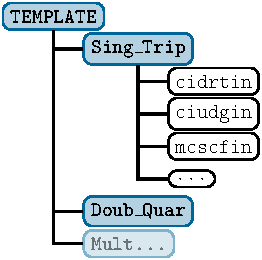
\includegraphics[scale=1]{img/dirs_COLtemp/dirs_COLtemp.pdf}
  \caption{Example directory structure of the \textsc{Columbus} template directory}
  \label{fig:dirs_COLtemp}
\end{figure}






% ========================================================================================================= %

\section{Analytical PESs Interface}\label{sec:int:analytical}

The \sharc\ suite also contains an interface which allows to run dynamics simulations on PESs expressed with analytical functions.
In order to allow dynamics simulations in the same way as it is done on-the-fly, the interface uses two kinds of potential couplings:
\begin{itemize}
  \item couplings that are pre-diagonalized in the interface (yielding the equivalent of the MCH basis),
  \item couplings given by the interface to \sharc\ as off-diagonal elements.
\end{itemize}

The interface needs one additional input file, called \ttt{SH2Ana.inp}, which contains the definitions of all analytical expressions.

\subsection{Parametrization}

The interface has to be provided with analytical expressions for all matrix elements of the following matrices in the diabatic basis:
\begin{itemize}
  \item Hamiltonian: $\mathbf{H}$
  \item Derivative of the Hamiltonian with respect to each atomic coordinate: $\mathbf{H}_{x_i}$
  \item (Transition) dipole matrices for each polarization direction: $\mathbf{M}_i$
  \item Real and imaginary part of the SOC matrix: $\boldsymbol{\Sigma}$
  \item (Optionally) the derivatives of the transition dipole matrices: $\mathbf{D}_{i,x_j}$
\end{itemize}

The diabatic Hamiltonian is diagonalized:
\begin{equation}
  \mathbf{H}^{\text{d}}=\mathbf{W}^\dagger\mathbf{H}\mathbf{W}
\end{equation}


Then the following calculations lead to the MCH matrices which are passed to \sharc:
\begin{align}
  \mathbf{H}^{\text{MCH}}&=\mathbf{H}^{\text{d}}+\mathbf{W}^\dagger\boldsymbol{\Sigma}\mathbf{W}\\
  \left(\mathbf{g}^{\text{MCH}}_\alpha\right)_{x_i}&=\left(\mathbf{W}^\dagger\mathbf{H}_{x_i}\mathbf{W}\right)_{\alpha\alpha}\\
  \mathbf{M}^{\text{MCH}}_i&=\mathbf{W}^\dagger\mathbf{M}_i\mathbf{W}\\
  \mathbf{S}^{\text{MCH}}(t_0,t)&=\mathbf{W}^\dagger(t_0)\mathbf{W}(t)\\
  \mathbf{D}^{\text{MCH}}_{i,x_j}&=\mathbf{W}^\dagger\mathbf{D}_{i,x_j}\mathbf{W}
\end{align}
The MCH Hamiltonian is the diagonalized diabatic Hamiltonian plus the SO matrix transformed into the MCH basis. The gradients in the MCH basis are obtained by transforming the derivative matrices into the MCH basis. The dipole matrices are also simply transformed into the MCH basis. The overlap matrix is the overlap of old and new transformation matrix.

\subsection{Interface-specific input file}

The interface-specific input file is called \ttt{SH2Ana.inp}. It contains the analytical expressions for all matrix elements mentioned above. All analytical expressions in this file are evaluated considering the atomic coordinates read from \ttt{QM.in}.

The file consists of a file header and the file body. The file body consists of variable definition blocks and matrix blocks.

\paragraph{Header} 

The header looks similar to an xyz file:
\begin{example}
  \begin{verbatim}
2
2
I       xI       0       0
Br      xBr      0       0
  \end{verbatim}
\end{example}
Here, the first line gives the number of atoms and the second line the number of states. 

On the remaining lines, each cartesian component of the atomic coordinates is associated to a variable name, which can be used in the analytical expressions. If a zero (\ttt{0}) is given instead of a variable name, then the corresponding cartesian coordinate is neglected. In the above example, the variable name \ttt{xI} is associated with the $x$ coordinate of the first atom given in \ttt{QM.in}. The $y$ and $z$ coordinates of the first atom are neglected.

All variable names must be \href{https://docs.python.org/2/reference/lexical_analysis.html#identifiers}{valid Python identifiers} and must not start with an underscore. Hence, all strings starting with a letter, followed by an arbitrary number of letters, digits and underscores, are valid. It is not allowed to use a variable name twice.

Note that the file header also contains the atom labels, which are just used for cross-checking against the atom labels in \ttt{QM.in}.

The file header must not contain comments, neither at the end of a line nor separate lines. Also, blank lines are not allowed in the header. After the last line of the header (where the variables for the $n_{\text{atom}}$-th atom are defined), blank lines and comments can be used freely (except in matrix blocks).

\paragraph{Variable definition blocks}

Variable definition blocks can be used to store additional numerical values (beyond the atomic coordinates) in variables, which can then be used in the equations in the matrix blocks. The most obvious use for this is of course to define values which will appear several times in the equations.

A variable definition block looks like:
\begin{example}
  \begin{verbatim}
Variables
A1      0.067
g1      0.996   # Trailing comment
# Blank line with comment only
R1      4.666
End
  \end{verbatim}
\end{example}
Each block starts with the keyword ``Variables'' and is terminated with ``End''. Inbetween, on each line a variable name and the corresponding numerical value (separated by blanks) can be given. Note that the naming conventions given above also apply to variables defined in these blocks. 

There can be any number of complete variable definitions blocks in the input file. All blocks are read first, before any matrix expressions are evaluated. Hence, the relative order of the variable blocks and the matrix blocks does not matter. Also, note that variable names must not appear twice, so variables cannot be redefined halfway through the file.

\paragraph{Matrix blocks}

The most important information in the input file are of course contained in the expressions in the matrix blocks. In general, a matrix block has the following format:
\begin{example}
  \begin{verbatim}
Matrix_Identifier
V11
V12,    V22
V13,    V23,    V33
...
  \end{verbatim}
\end{example}
The first line identifies the type of matrix. Those are valid identifiers:

\begin{tabular}{p{5cm}p{9cm}}
\ttt{Hamiltonian}                               &Defines the Hamiltonian including the diabatic potential couplings.\\
\ttt{Derivatives} followed by a variable name   &Derivative of the Hamiltonian with respect to the given variable.\\
\ttt{Dipole} followed by 1, 2 or 3              &(Transition) dipole moment matrix for cartesian direction $x$, $y$ or $z$, respectively.\\
\ttt{Dipolederivatives} followed by 1, 2 or 3 followed by a variable name       &Derivative of the respective dipole moment matrix.\\
\ttt{SpinOrbit} followed by \ttt{R} or \ttt{I}  &Real or Imaginary (respectively) part of the spin-orbit coupling matrix $\boldsymbol{\Sigma}$.\\
\end{tabular}

Since the interface searches the file for these identifiers starting from the top until it is found, for each matrix only the first block takes effect. Note that the Hamiltonian and all relevant derivatives must be present. If dipole matrix, dipole derivative matrix or SO matrix definitions are missing, they will be assumed zero.

In the lines after the identifier, the expressions for each matrix element are given. Note the lower triangular format (all matrices are assumed symmetric, except the imaginary part of the SO matrix, which is assumed antisymmetric). Matrix elements must be separated by commas (so that whitespace can be used inside the expressions). There must be at least as many lines as the number of states (additional lines are neglected). If any line or matrix element is missing, the interface will abort.

An examplary block looks like:
\begin{example}
  \begin{verbatim}
Hamiltonian
A1*( (1.-math.exp(g1*(R1-xI+xBr)))**2-1.),
0.0006,                                         3e-5*(xI-xBr)**2
  \end{verbatim}
\end{example}
It is important to understand that the expressions are directly evaluated by the Python interpreter, hence all expressions must be valid Python expressions which evaluate to numeric (integer or float) values. Only the variables defined above can be used. 

Note that exponentiation in Python is \ttt{**}. In order to provide most usual mathematical functions, the \href{https://docs.python.org/2/library/math.html}{\ttt{math} module} is available. Among others, the \ttt{math} module provides the following functions:
\begin{itemize}
  \item \ttt{math.exp(x)}: Exponential function
  \item \ttt{math.log(x)}: Natural logarithm
  \item \ttt{math.pow(x,y)}: $x^y$
  \item \ttt{math.sqrt(x)}: $\sqrt{x}$
  \item \ttt{math.cos(x)}, \ttt{math.sin(x)}, \ttt{math.tan(x)}
  \item \ttt{math.acos(x)}, \ttt{math.asin(x)}, \ttt{math.atan(x)}
  \item \ttt{math.atan2(y,x)}: $\tan^{-1}\left(\frac{y}{x}\right)$, as in many programming languages (takes care of phases)
  \item \ttt{math.pi}, \ttt{math.e}: $\pi$ and Euler's number
  \item \ttt{math.cosh(x)}, \ttt{math.sinh(x)}: Hyperbolic functions (also tanh, acosh, asinh, atanh are available)
\end{itemize}



% ========================================================================================================= %
% ========================================================================================================= %
% ========================================================================================================= %

\chapter{Auxilliary Scripts}\label{chap:aux}

In this chapter, all auxiliary scripts and programs are documented. Input generators (currently \ttt{molpro\_input.py} and \ttt{molcas\_input.py}) are documented in the relevant interface sections.

All auxiliary scripts are either interactive -- prompting user input from stdin in order to setup a certain task -- or non-interactive, meaning they are controlled by command-line arguments and options, in the same way as many command-line tools work.

All interactive scripts sequentially ask a number of questions to the user. In many cases, a default value is presented, which is either preset or detected by the scripts based on the availability of certain files. Furthermore, the scripts feature auto-completion of paths and filenames (use TAB), which is active only in questions where auto-completion is relevant.

All interactive scripts write a file called \ttt{KEYSTROKES.<script\_name>} which contains the user input from the last completed session. These files can be piped to the interactive scripts to perform the same task again, for example:
\begin{verbatim}
user@host> cat KEYSTROKES.excite - | $SHARC/excite.py
\end{verbatim}
Note the \ttt{-}, which tells \ttt{cat} to switch to stdin after the file ends, so that the user can proceed if the script asks for more input than contained in the \ttt{KEYSTROKES} file.

All non-interactive scripts can be called with the \ttt{-h} option to obtain a short description, usage information and a list of the command line options.

All scripts can be safely killed during a run by using \ttt{CTRL+C}. In the case of interactive scripts, a \ttt{KEYSTROKES.tmp} file remains, containing the user input made so far.

\section{Wigner Distribution Sampling: \ttt{wigner.py}}\label{sec:wigner.py}

The first step in preparing the dynamics calculation is to obtain a set of physically reasonable initial conditions. Each initial condition is a set of initial atomic coordinates, initial atomic velocities and initial electronic state. The initial geometry and velocities can be obtained in different ways. With \sharc, usually sampling of a quantum-harmonic Wigner distribution is performed. 

The sampling is carried out with the non-interactive Python script \ttt{wigner.py}. The theoretical background is summarized in section~\ref{met:wigner}.

\subsection{Usage}

The general usage is 
\begin{verbatim}
user@host> python $SHARC/wigner.py [options] filename.molden
\end{verbatim}
\ttt{wigner.py} takes exactly one command-line argument (the input file with the frequencies and normal modes), plus some options. Usually, the \ttt{-n} option is necessary, since by default only 3 initial conditions are created.

The argument is the filename of the file containing the information about the vibrational frequencies and normal modes. The file is by default assumed to be in the \href{http://www.cmbi.ru.nl/molden/molden_format.html}{\textsc{Molden} format}. For usage with \ttt{wigner.py}, only the following blocks have to be present:

\begin{minipage}{0.9\textwidth}
  \begin{itemize}
    \item $[$FREQ$]$
    \item $[$FR-COORD$]$
    \item $[$FR-NORM-COORD$]$
  \end{itemize}
\end{minipage}

Alternatively, the information about the vibrational frequencies and normal modes can be read directly from a \textsc{Molpro} output file of a frequency calculation. In this case, in addition to the filename also the switch \ttt{-M} has to be given:
\begin{verbatim}
user@host> python $SHARC/wigner.py -M MOLPRO.out
\end{verbatim}

The script accepts a number of command-line options, specified in table~\ref{tab:wigner_opts}.
\begin{table}
  \centering
  \caption{Command-line options for script \ttt{wigner.py}.}
  \label{tab:wigner_opts}
  \begin{tabular}{>{\tt}lll}
    \toprule
    \rmfamily Option        &Description      &Default\\
    \midrule
    -h                  &Display help message and quit.             & --                             \\
    -m                  &Modify atom masses                         &Most common isotope.           \\
    -M                  &Assume a \textsc{Molpro} input file.       &Assume a \textsc{Molden} file. \\
    -n  INTEGER         &Number of initial conditions to generate.  &3                              \\
    -o  FILENAME        &Output filename.                           &\ttt{initconds}                \\
    -r  INTEGER         &Seed for random number generator.          &16661                          \\
    -s  FLOAT           &Scaling factor for the frequencies.        &1.0                            \\
    \bottomrule
  \end{tabular}
\end{table}

\subsection{Output}

The script \ttt{wigner.py} generates a single output file, by default called \ttt{initconds}. All information about the initial conditions is stored in this file. Later steps in the preparation of the initial conditions add information about the excited states to this file. The file is formatted in a human-readable form.

The \ttt{initconds} file format is specified in section~\ref{sec:initcondsfile}.

\subsection{Non-default Masses}

When the \ttt{-m} option is used, the script will ask the user to interactively modify the atom masses. For each atom (referred to by the atom index as in the \textsc{Molden} file), a mass can be given (relative atomic weights). Note that the frequency calculation which produces the \textsc{Molden} or \textsc{Molpro} file should be done with the same atomic masses.

\section{Setup of Initial Calculations: \ttt{setup\_init.py}}\label{sec:setup_init.py}

The interactive script \ttt{setup\_init.py} creates input for singlepoint calculations at the initial geometries given in an \ttt{initconds} file. These calculations might be necessary for some schemes to select the initial electronic state of the trajectory, based on the excitation energies and oscillator strength of the transitions from ground state to the excited state under consideration. 

There are other choices of the initial state possible, which do not require singlepoint calculations at all initial geometries. See the description of \ttt{excite.py} (section~\ref{sec:excite.py}). In this case, \ttt{setup\_init.py} can be used to set up only the calculation at the equilibrium geometry (see below at ``Range of Initial Conditions'').

\subsection{Usage}

The script is interactive, and can be started by simply typing 
\begin{verbatim}
user@host> python $SHARC/setup_init.py
\end{verbatim}
Please be aware that the script will setup the calculations in the directory where it was started, so the user should \ttt{cd} to the desired directory before executing the script.

Please note that the script does not expand \ttt{\textasciitilde} or shell variables, except where noted otherwise.

\subsection{Input}

The script will prompt the user for the input. In the following, all input parameters are documented:

\paragraph{Initial Conditions File}

Enter the filename of the initial conditions file, which was generated beforehand with \ttt{wigner.py}. If the script finds a file called \ttt{initconds}, the user is asked whether to use this file, otherwise the user has to enter an appropriate filename. The script detects the number of initial conditions and number of atoms automatically from the initial conditions file.

\paragraph{Range of Initial Conditions}

The initial conditions in \ttt{initconds} are indexed, starting with the index 1. In order to prepare ab initio calculations for a subset of all initial conditions, enter a range of indices, e.g.\ $a$ and $b$. This will prepare all initial conditions with indices in the interval $[a,b]$. In any case, the script will additionally prepare a calculation for the equilibrium geometry (except if a finished calculation for the equilibrium geometry was found).

If the interval $[0,0]$ is given, the script will only setup the calculation at the equilibrium geometry.

\paragraph{Number of states}

Here the user can specify the number of excited states to be calculated. Note that the ground state has to be counted as well, e.g.\ if 4 singlet states are specified, the calculation will involve the $S_0$, $S_1$, $S_2$ and $S_3$. Also states of higher multiplicity can be given, e.g.\ triplet or quintett states. 
For even-electron molecules, including odd-electron states (e.g.\ doublets) is only useful if transition properties for ionization can be computed (e.g.\ Dyson norms with the \textsc{Columbus} interface). These transition properties can be used to calculate ionization spectra or to obtain initial conditions for dynamics after ionization.

\paragraph{Spin-orbit calculation}

Usually it is sufficient to calculate the spin-free excitation energies and oscillator strengths in order to decide for the initial state. However, using this option, the effects of spin-orbit coupling on the excitation energies and oscillator strengths can be included. Note that the script will never calculate spin-orbit couplings if only singlet states are included in the calculation.

\paragraph{Interface}

In this point, choose any of the displayed interfaces to carry out the ab initio calculations. Enter the corresponding number. 

The following input section depends on the chosen interface.

\subsection{Input for \textsc{Molpro}}\label{sec:setup_init.py:molpro}

\paragraph{Path to \textsc{Molpro}}

Here the user is prompted to provide the path to the \textsc{Molpro} executable. 

Note that the setup script will not expand the user (\ttt{\textasciitilde}) and shell variables (since the calculations might be running on a different machine than the one used for setup, so the meaning of shell variables could be different). \ttt{\textasciitilde} and shell variables will only be expanded by the interfaces during the actual calculation.

\paragraph{Scratch directory}

The script takes the string without any checking. Each individual initial condition uses a subdirectory \ttt{ICOND\_\%05i} with the appropriate number. \ttt{\textasciitilde} and shell variables will only be expanded by the interface during the actual calculation.

Note that you can use, e.g., \ttt{./temp/} as scratch directory, which is a subdirectory of the working directory of the interface. Using \ttt{./} as scratch directory is not recommended, since the interface will delete the scratch directory.

\paragraph{Template file}

Enter the filename for the \textsc{Molpro} template input. This file contains the details of the ab initio calculation, like basis set, active orbitals and electrons, number of electrons and number of states for state-averaging. For \textsc{Molpro}, it also contains the memory usage. For details, see the section about the \sharc-\textsc{Molpro} interface (\ref{sec:int:molpro}). The setup script will check whether the template file contains the necessary entries. 

\paragraph{Initial wavefunction file}

You can provide an initial wavefunction (with an appropriate MO guess) to \textsc{Molpro}. This usually provides a drastic speedup for the CASSCF calculations and helps in ensuring that all calculations are based on the same active space. In simple cases it might be acceptable to not provide an initial wavefunction.

\subsection{Input for \textsc{Columbus}}

\paragraph{Path to \textsc{Columbus}}

Here the user is prompted to provide the path to the \textsc{Columbus} directory. Note that the script will not expand the user (\ttt{\textasciitilde}) and shell variables (since possibly the ab initio calculations are running on a different machine than the one used for setup). \ttt{\textasciitilde} and shell variables will only be expanded by the interfaces during the actual calculation.

Note that \ttt{\$COLUMBUS} does not have to be defined on the setup host, but it has to be defined on the hosts running the calculations.

\paragraph{Scratch directory}

The script takes the string without any checking. Each individual initial condition uses a subdirectory \ttt{ICOND\_\%05i} with the appropriate number. \ttt{\textasciitilde} and shell variables will only be expanded by the interface during the actual calculation.

Note that you can use, e.g., \ttt{./temp/} as scratch directory, which is a subdirectory of the working directory of the interface. Using \ttt{./} as scratch directory is not recommended, since the interface will delete the scratch directory.

\paragraph{Template directory}

Enter the path to a directory containing subdirectories with \textsc{Columbus} input files necessary for the calculations. The setup script will expand \ttt{\textasciitilde} and shell variables and will pass the absolute path to the calculations.

The script will auto-detect (based on the \ttt{cidrtin} files) which subdirectory contains the input for each multiplicity. The user has to check in the following dialog whether the association of multiplicities with job directories is correct. Additionally, the association of MO coefficient files to the jobs has to be checked. See the section on the \sharc-\textsc{Columbus} interface (\ref{sec:int:columbus}) for further details. 

Note that the setup script does not check any content of the input files beyond the multiplicity. Note that \ttt{transmomin} and \ttt{control.run} do not need to be present (and that their content has no effect on the calculation), since these files are written on-the-fly by the interface. 

\paragraph{Initial orbital coefficient file}

You can provide initial MO coefficients for the \textsc{Columbus} calculation. This usually provides a drastic speedup for the CASSCF calculations and helps to ensure that all calculations are based on the same active space. In simple cases it might be acceptable to not provide an initial wavefunction.

\paragraph{Memory}

For \textsc{Columbus}, the available memory must be given here. 

\subsection{Input for \textsc{Molcas}}

\paragraph{Path to \textsc{Molcas}}

The script will first look for a shell variable \ttt{\$MOLCAS}. The user can either confirm that \ttt{\$MOLCAS} is the correct executable, or enter the correct path. Note that the setup script will not expand the user (\ttt{\textasciitilde}) and shell variables (since possibly the ab initio calculations are running on a different machine than the one used for setup). The \sharc-\textsc{Molcas} interface will expand \ttt{\textasciitilde} and shell variables.

\paragraph{Scratch directory}

The script takes the string without any checking. Each individual initial condition uses a subdirectory \ttt{ICOND\_\%05i} with the appropriate number. \ttt{\textasciitilde} and shell variables will only be expanded by the interface during the actual calculation.

Note that you can use, e.g., \ttt{./temp/} as scratch directory, which is a subdirectory of the working directory of the interface. Using \ttt{./} as scratch directory is not recommended, since the interface will delete the scratch directory.

\paragraph{Template file}

Enter the filename for the \textsc{Molcas} template input. This file contains the details of the ab initio calculation, like basis set, active orbitals and electrons, number of electrons and number of states for state-averaging. For details, see the section about the \sharc-\textsc{Molcas} interface (\ref{sec:int:molcas}). The setup script will check whether the template file contains the necessary entries. 

\paragraph{Initial wavefunction file}

You can provide initial MO coefficients to \textsc{Molcas}. This usually provides a drastic speedup for the CASSCF calculations and helps in ensuring that all calculations are based on the same active space. In simple cases it might be acceptable to not provide an initial wavefunction. For \textsc{Molcas}, you have to specify one file for each multiplicity.



\subsection{Input for analytical potentials}\label{sec:setup_init.py:analytical}

\paragraph{Template file}

Enter the filename for the template input specifying the analytical potentials. For details, see the section about the \sharc-Analytical interface (\ref{sec:int:analytical}). The setup script will check whether the template file is valid. 



\subsection{Input for Run Scripts}\label{sec:setup_init.py:run}

\paragraph{Run script mode}

The script \ttt{setup\_init.py} generates a run script (Bash) for each initial condition calculation. Due to the large variety of cluster architectures, these run scripts might not work in every case. It is the user's responsibility to adapt the generated run scripts to his needs.

\ttt{setup\_init.py} can generate run scripts for two different schemes how to execute the calculations. With the first scheme, the ab initio calculations are performed in the directory where they were setup (subdirectories of the directory where \ttt{setup\_init.py} was started). Note that the interfaces will still use their scratch directories to perform the actual quantum chemistry calculations.

With the second option, the run scripts will transfer the input files for each ab initio calculation to a temporary directory, where the interface is started. After the interface finishes all calculations, the results files are transferred back to the primary directory and the temporary directory is deleted. Note that \ttt{setup\_init.py} in any case creates the directory structure in the directory where it was started. The name of the temporary directory can contain shell variables, which will be expanded when the script is running (on the compute host).

\paragraph{Submission script}

The setup script can also create a Bash script for the submission of all ab initio calculations to a queueing system. The user has to provide a submission command for that, including any options which might be necessary. This submission script might not work with all queueing systems.

\paragraph{Project name}

The user can enter a project name. This is used currently only for the job names of submitted jobs (\ttt{-N} option for queueing system).

\subsection{Output}

\ttt{setup\_init.py} will create for each initial condition in the given range a directory whose names follow the format \ttt{ICOND\_\%05i}, where \ttt{\%05i} is the index of the initial condition padded with zeroes to 5 digits. Additionally, the directory \ttt{ICOND\_00000} is created for the calculation of the excitation energies at the equilibrium geometry.

To each directory, the following files will be added:
\begin{itemize}
  \item \ttt{QM.in}: Main input file for the interface, contains the geometry and the control keywords (to specify which quantities need to be calculated). 
  \item \ttt{run.sh}: Run script, which can be started interactively in order to perform the ab initio calculation in this directory. Can also be adapted to a batch script for submission to a queue 
  \item Interface-specific files: Usually a template file, a file containing additional input for the interface, and an initial wavefunction.
\end{itemize}

The calculations in each directory can be simply executed by starting \ttt{run.sh} in each directory. In order to perform this task consecutively on a single machine, the script \ttt{all\_run.sh} can be executed. The file \ttt{DONE} contains the progress of this calculation.
Alternatively, each run script can be sent to a queueing system (you might need to adapt this script to you cluster system).

In figure~\ref{fig:dirs_init}, the directory tree structure setup by \ttt{setup\_init.py} is given.

\begin{figure}
  \centering
  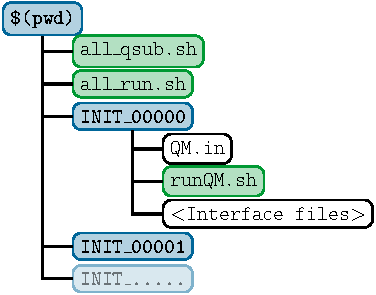
\includegraphics[scale=1]{img/dirs_init/dirs_init.pdf}
  \caption{Directory structure created by \ttt{setup\_init.py}. Directories are in blue, executable scripts in green and regular files in black and white. Interface files usually include initial MO coefficients, template files and interface input files.}
  \label{fig:dirs_init}
\end{figure}

After all calculations are finished, \ttt{excite.py} can be used to collect the results.


\section{Excitation Selection: \ttt{excite.py}}\label{sec:excite.py}

\ttt{excite.py} has two tasks: adding excited-state information to the \ttt{initconds} file, and deciding which excited state for which initial condition is a valid initial state for the dynamics.


\subsection{Usage}

The script is interactive, and can be started by simply typing 
\begin{verbatim}
user@host> python $SHARC/excite.py
\end{verbatim}


\subsection{Input}

\paragraph{Initial condition file}

Enter the path to the initial conditions file, to which \ttt{excite.py} will add excited-state information. This file can already contain excited-state information (in this case this information can be reused).

\paragraph{Generate excited state list}

There are three possibilities to add excited-state information to the \ttt{initconds} file:
\begin{enumerate}
  \item generate a list of dummy excited states,
  \item read excited-state information from the output of the initial ab initio calculations (prepare the calculations with \ttt{setup\_init.py}),
  \item keep the existing excited-state information in the \ttt{initconds} file.
\end{enumerate}
The first option is mainly used if no initial ab initio calculations need to be performed (e.g., the initial state is known). 

In order to use the second option, one should first setup initial excited-state calculations using \ttt{setup\_init.py} (see~\ref{sec:setup_init.py}) and run the calculations. \ttt{excite.py} can then read the output of the initial calculations and calculate excitation energies and oscillator strengths.

The third option can be used to reuse the information in the \ttt{initconds} file, e.g., to apply a different selection scheme to the states or to just read the number of states.

\paragraph{Path to ab initio results}

If \ttt{excite.py} will read the excited-state information from the ab initio calculation results, here the user has to provide the path to the directory containing the \ttt{ICOND\_\%05i} subdirectories.

\paragraph{Number of states}

If a dummy list of states will be generated, the user has to provide the number of states per multiplicity. Note that a singlet ground state has to be counted as well, e.g.\ if 4 singlet states are specified, the calculation will involve the $S_0$, $S_1$, $S_2$ and $S_3$. Also states of higher multiplicity can be given, e.g.\ doublet or triplet states (e.g., \ttt{2 2 1} for two singlets, two doublets and one triplet).

If the ab initio results are read the number of states will be automatically determined from the results.

\paragraph{Excited-state representation}

When generating new lists of excited states (either dummy states or from ab initio results), the user has to specify the representation of the excited states (either MCH or diagonal representation). The MCH representation is spin-free, meaning that transition dipole moments are only allowed between states of the same multiplicity. For molecules without heavy atoms, this option is sufficient. For heavier atoms, the diagonal representation can be used, which includes the effects of spin-orbit coupling on the excitation energies and oscillator strengths. 

When reading ab initio results, \ttt{excite.py} will diagonalize the Hamiltonian and transform the transition dipole matrices for each initial condition to obtain the diagonal representation. 

When a dummy state list is generated, the representation will only be written to the output file \ttt{initconds.excited} (but has no actual numeric effect for \ttt{excite.py}). Note that the representation which is declared in the \ttt{initconds.excited} file influences how \sharc\ determines the initial coefficients (see the paragraph on initial coefficients in~~\ref{ssec:input:keywords}).

Note that the representation cannot be changed if existing excited-state information is kept. 

Hint: If the \ttt{ICOND\_\%05i} directories need to be deleted (e.g., due to disk space restrictions), making one read-out with \ttt{excite.py} for each representation and saving the results to two different files will preserve all necessary information.

\paragraph{Ionization probabilities}

If \ttt{excite.py} detects that the ab initio results contain ionization probabilities, then those can be used instead of the transition dipole moments. Note that in this case the transition dipole moments are not written to the \ttt{initconds.excited} file. 

\paragraph{Reference energy}

\ttt{excite.py} can read the reference energy (ground state equilibrium energy) directly from the ab initio results. If the ab initio data is read anyways, \ttt{excite.py} already knows the relevant path. If a dummy list of states is generated, the user can provide just the path to the \ttt{QM.out} file of the ab initio calculation for the equilibrium geometry. Otherwise, \ttt{excite.py} will prompt the user to enter a reference energy manually (in hartree).

\paragraph{Initial state selection}

Every excited state of each initial condition has a flag specifying it either as a valid initial state or not. \ttt{excite.py} has four modes how to flag the excited states:
\begin{enumerate}
  \item Unselect all excited states,
  \item User provides a list of initial states,
  \item States are selected stochastically based on excitation energies and oscillator strengths,
  \item Keep all existing flags.
\end{enumerate}
The first option can be used if \ttt{excite.py} is only used to read the ab initio results for the generation of an absorption spectrum (using \ttt{spectrum.py}). 

The second option can be used to directly specify a list of initial states, if the initial state is known (e.g., starting in the ground state and exciting with an explicit laser field). In this case, the given states of \textit{all} initial conditions are flagged as initial states.

The third option is only available if excited-state information exists (i.e., if no dummy list is generated). For details on the stochastic selection procedure, see section~\ref{met:exc_selection}. 

The fourth option can only be used if the existing state information is kept. In this case \ttt{excite.py} does nothing except counting the number of flagged initial states.

\paragraph{Excitation window}

This option allows to exclude excited states from the selection procedure if they are outside a given energy window. This option is only available if excited state information exists, but not if a dummy list of states is generated (because the dummy states have no defined excitation energy).

For the stochastic selection procedure, states outside the excitation window do not count for the determination of $p_\text{max}$ (see equation~\eqref{eq:exc_prob}). This allows to excite, e.g., to a dark $n\pi^*$ state despite the presence of a much brighter $\pi\pi^*$ state.

For the keep-flags option, this option can be used to count the number of excited states in the energy window.

\paragraph{Considered states}

Here the user can specify the list of desired initial states. 
For the stochastic selection procedure, the user can instead exclude certain states from the procedure. Excluded states do not count for the determination of $p_\text{max}$ (see equation~\eqref{eq:exc_prob}).

If the number of states per multiplicity is known, \ttt{excite.py} will print a table giving for each state index the multiplicity, quantum number and $M_s$ value.


\paragraph{Random number generator seed}

The random number generator in \ttt{excite.py} is used in the stochastic selection procedure. Instead of typing an integer, typing ``\ttt{!}'' will initialize the RNG from the system time. Note that this will not be reproducible, i.e.\ repeating the \ttt{excite.py} run with ``\ttt{!}'' as random seed will give a different selection in each run.



\subsection{Matrix diagonalization}

When using the diagonal representation, \ttt{excite.py} needs to diagonalize and multiply matrices. By default, the Python package \textsc{NumPy} is used, if available. If the script does not find a \textsc{NumPy} installation, it will use a small Fortran code which comes with the \sharc\ suite. In order for this to work, you need to set the environment variable \ttt{\$SHARC} to the \ttt{bin/} directory within your \sharc\ installation. See section~\ref{sec:diagonalizer.x} for more details.

\subsection{Output}

\ttt{excite.py} writes all output to a file \ttt{<BASE>.excited}, where \ttt{<BASE>} is the name of the initial conditions file used as input. The output file is also an initial conditions file, but contains additional information regarding the excited states, the reference energy and the representation of the excited states. An initial conditions file with excited-state information is needed for the final preparatory step: setting up the dynamics with \ttt{setup\_traj.py}.
Additionally, \ttt{spectrum.py} can calculate absorption spectra from excited-state initial condition files.

\subsection{Specification of the \ttt{initconds.excited} file format}\label{sec:initcondsfile}

The initial conditions files \ttt{initconds} and \ttt{initconds.excited} contain lists of initial conditions, which are needed for the setup of trajectories. An initial condition is a set of initial coordinates of all atoms and corresponding initial velocities of each atom, and optionally a list of excited state informations. In the following, the format of this file is specified.

The file contains of a header, followed by the body of the file containing a list of the initial conditions. 

\paragraph{File header}

An examplary header looks like:
\begin{example}
\footnotesize\begin{verbatim}
SHARC Initial conditions file, version 0.2   <Excited>
Ninit     100
Natom     2
Repr      MCH
Eref         -0.50
Eharm           0.04
States    2 0 1 

Equilibrium
 H   1.0  0.0  0.0  0.0   1.00782503   0.0  0.0  0.0
 H   1.0  1.5  0.0  0.0   1.00782503   0.0  0.0  0.0
\end{verbatim}
\end{example}
The first line must read \ttt{SHARC Initial conditions file, version <VERSION>}, with the correct version string followed. The string \ttt{Excited} is optional, and marks an initial conditions file as being an output file of \ttt{excite.py} (\ttt{setup\_traj.py} will only accept files marked like this). The following lines contain:
\begin{enumerate}
  \item the number of initial conditions, 
  \item the number of atoms,
  \item the electronic state representation (a string which is \ttt{None}, \ttt{MCH} or \ttt{diag}),
  \item the reference energy (hartree),
  \item the harmonic energy (zero point energy in the harmonic approximation, hartree),
  \item optionally the number of states per multiplicity.
\end{enumerate}

After the header, first the equilibrium geometry is expected. It is demarked with the keyword \ttt{Equilibrium}, followed by $n_\text{atom}$ lines, each specifying one atom. Unlike the actual initial conditions, the equilibrium geometry does not have a list of excited states or defined energies.

\paragraph{File body}

The file body contains a list of initial conditions. Each initial condition is specified by a block starting with a line containing the string \ttt{Index} and the number of the initial condition. In the file, the initial conditions are expected to appear in order.

A block specifying an initial condition looks like:
\begin{example}
\footnotesize\begin{verbatim}
Index     1
Atoms
 H   1.0  -0.02  0.0  0.0   1.00782503  -0.001  0.0  0.0
 H   1.0   1.52  0.0  0.0   1.00782503   0.001  0.0  0.0
States
001    -0.49    -0.49  -0.16   0.0  -0.03   0.0   0.05   0.0   0.0   0.00 False
002    -0.25    -0.49   0.02   0.0   0.43   0.0  -1.77   0.0   6.5   0.53 True
003    -0.40    -0.49   0.00   0.0   0.00   0.0   0.00   0.0   2.5   0.00 False
004    -0.40    -0.49   0.00   0.0   0.00   0.0   0.00   0.0   2.5   0.00 False
005    -0.40    -0.49   0.00   0.0   0.00   0.0   0.00   0.0   2.5   0.00 False
Ekin        0.004 a.u.
Epot_harm   0.026 a.u.
Epot        0.013 a.u.
Etot_harm   0.030 a.u.
Etot        0.018 a.u.
\end{verbatim}
\end{example}
The formal structure of such a block is as follows. After the line containing the keyword \ttt{Index} and the index number, the keyword \ttt{Atoms} indicates the start of the list of atoms. Each atom is specified on one line:
\begin{enumerate}
  \item symbol,
  \item nuclear charge,
  \item $x$, $y$, $z$ coordinate in Bohrs,
  \item atomic mass,
  \item $x$, $y$ and $z$ component of nuclear velocity in atomic units.
\end{enumerate}

After the atom list, the keyword \ttt{States} indicates the list of electronic states. This list consists of one line per electronic state, but can be empty, if no information of the electronic states is available. Each line consists of: 
\begin{enumerate}
  \item state number (starting with 1),
  \item state energy in Hartree, 
  \item reference energy in Hartree (usually the energy of the lowest state),
  \item six numbers defining the transition dipole moment to the reference state (usually the lowest state),
  \item the excitation energy in eV,
  \item the oscillator strength,
  \item a string which is either \ttt{True} or \ttt{False}, specifying whether the electronic state was selected by \ttt{excite.py} as initial electronic state. 
\end{enumerate}
The transition dipole moments are specified by six floating point numbers, which are real part of the $x$ component, imaginary part of the $x$ component, then the real and imaginary parts for the $y$ and finally the $z$ component (the transition dipole moments can be complex in the diagonal representation). 

The electronic state list is terminated with the keyword \ttt{Ekin}, which at the same time gives the kinetic energy of all atoms. The remaining entries give the potential energy in the harmonic approximation and the actual potential energy, as well as the total energy.





\section{Setup of Trajectories: \ttt{setup\_traj.py}}\label{sec:setup_traj.py}

This interactive script prepares the input for the excited-state dynamics simulations with \sharc. It works similarly to \ttt{setup\_init.py}, reading an initial conditions file, prompting the user for a number of input parameters, and finally prepares one directory per trajectory. However, the \ttt{setup\_traj.py} input section is noticeably longer, because many options for the dynamics are covered.

\subsection{Input}

\paragraph{Initial conditions file}

Please be aware that \ttt{setup\_traj.py} needs an initial conditions file generated by \ttt{excite.py} (Files generated by \ttt{wigner.py} are not allowed). The script reads the number of initial states, the representation and the reference energy automatically from the file.

\paragraph{Number of states}

This is the total number of states per multiplicity included in the dynamics calculation. Affects the keyword \ttt{nstates} in the \sharc\ input file.

Only advanced users should use here a different number of states than given to \ttt{setup\_init.py}. In this case, the excited-state information in the initial conditions file might be inconsistent. For example, if 10 singlets and 10 triplets were included in the initial calculations, but only 5 singlets and 5 triplets in the dynamics, then the sixth entry in the initial conditions file corresponds to $S_5$, while \ttt{setup\_traj.py} assumes the sixth entry to correspond to $T_1$.

\paragraph{Active states}

States can be frozen for the dynamics calculation here. See section~\ref{met:activestates} for a general description of state freezing in \sharc. Only the highest states in each multiplicity can be frozen, it is not possible to, e.g., freeze the ground state in simulations where ground state relaxation is negligible. Affects the keyword \ttt{actstates}.

\paragraph{Contents of the initial conditions file}

Optionally, a map of the contents of the initial conditions file can be displayed during the execution of \ttt{setup\_traj.py}, showing for each state which initial conditions were selected (and which initial conditions do not have the necessary excited-state information). For each state, a table is given, where each symbol represents one initial condition. A dot ``\ttt{.}'' represents an initial condition where information about the current excited state is available, but which is not selected for dynamics. A hash mark ``\ttt{\#}'' represents an initial condition which is selected for dynamics. A question mark ``\ttt{?}'' represents initial conditions for which no information about the excited state is available (e.g.\ if the initial excited-state calculation failed). The tutorial shows an example of this output.

The content of the initial conditions file is also summarized in a table giving the number of initial conditions selected per state. 

\paragraph{Initial states for dynamics setup}

The user has to input all states from which trajectories should be launched. The numbers must be entered according to the above table giving the number of selected initial conditions per state. It is not allowed to specify inactive states as initial states. The script will give the number of trajectories which can be setup with the specified set of states. If no trajectories can be setup, the user has to specify another set of initial states. The initial state will be written to the \sharc\ input, specified in the same representation as given in the initial conditions file. The initial coefficients will be determined automatically by \sharc, according to the description in section~\ref{ssec:input:keywords}.

\paragraph{Starting index for dynamics setup}

Specifies the first initial condition within the initial condition file to be included in the setup. This is useful, for example, if the user might setup 50 trajectories starting with index 1. \ttt{setup\_traj.py} reports afterwards the last initial condition to be used for setup, e.g.\ index 90. Later, the user can setup additional trajectories, starting with index 91.

\paragraph{Random number generator seed}

The random number generator in \ttt{setup\_traj.py} is used to randomly generate RNG seeds for the \sharc\ input. Instead of typing an integer, typing ``\ttt{!}'' will initialize the RNG from the system time. Note that this will not be reproducible, i.e.\ repeating the \ttt{setup\_traj.py} run (with the same input) with ``\ttt{!}'' as random seed will give for the same trajectories different RNG seeds. Affects the keyword \ttt{RNGseed}.

\paragraph{Interface}

In this point, choose any of the displayed interfaces to carry out the ab initio calculations. Enter the corresponding number. The choice of the interface influences some dynamics options which can be set in the next section of the \ttt{setup\_traj.py} input.

\paragraph{Simulation Time}

This is the maximum time that \sharc\ will run the dynamics simulation. If trajectories need to be run for longer time, it is recommended to first let the simulation finish. Afterwards, increase the simulation time in the corresponding \sharc\ input file (keyword \ttt{tmax}) and add the restart keyword (also make sure that the \ttt{norestart} keyword is not present). Then the simulation can be restarted by running again the \ttt{run.sh} script. Sets the keyword \ttt{tmax} in the \sharc\ input files.

\paragraph{Simulation Timestep}

This gives the timestep for the dynamics. The on-the-fly ab initio calculations are performed with this timestep, as is the propagation of the nuclear coordinates. A shorter timestep gives more accurate results, especially if light atoms (hydrogen) are subjected to high kinetic energies or steep gradients. Of course a shorter timestep is computationally more expensive. A good compromise in many situations is 0.5~fs. Sets the keyword \ttt{stepsize} in the \sharc\ input files.

\paragraph{Number of substeps}

This gives the number of substeps for the interpolation of the Hamiltonian for the propagation of the electronic wavefunction. Usually, 25 substeps are sufficient. In cases where the diagonal elements of the Hamiltonian are very large (very large excitation energies or a badly chosen reference energy) more substeps are necessary. Sets the keyword \ttt{nsubsteps} in the \sharc\ input files.

\paragraph{Prematurely terminate trajectories}

Usually, trajectories which relaxed to the ground state do not recross to an excited state, but vibrate indefinitely in the ground state. If the user is not interested in these vibrations, such trajectories can be terminated prematurely in order to save computational ressources. A threshold of 10--20~fs is usually a good choice to safely detect ground state relaxation. Sets the keyword \ttt{killafter} in the \sharc\ input files.

\paragraph{Representation for the dynamics}

Either the diagonal representation can be chosen (by typing ``\ttt{yes}'') to perform dynamics with the \sharc\ methodology, or the dynamics can be performed on the MCH states (spin-diabatic dynamics \cite{Granucci2012JCP}, FISH \cite{Mitric2009PRA}). Sets the keyword \ttt{surf} in the \sharc\ input files.

\paragraph{Non-adiabatic couplings}

Electronic propagation can be performed with temporal derivatives, non-adiabatic coupling vectors or overlap matrices (Local diabatization). Enter the corresponding number. Note that depending on the chosen interface, some options might not be available, as displayed by \ttt{setup\_traj.py}. Sets the keyword \ttt{coupling} in the \sharc\ input files.

\paragraph{Gradient transformation}

The non-adiabatic coupling vectors can be used to correctly transform the gradients to the diagonal representation. If non-adiabatic coupling vectors are used anyways, this option is strongly recommended, since it gives more accurate gradients for no additional cost. Sets the keyword \ttt{gradcorrect} in the \sharc\ input files. If the dynamics uses the MCH representation, this question is not asked. 

\paragraph{Surface hop treatment}

This option determines how the total energy is conserved after a surface hop. Sets the keyword \ttt{ekincorrect} in the \sharc\ input files.

\paragraph{Decoherence correction}

For most applications, a decoherence correction should be enabled. Requesting decoherence correction here leads to the addition of the keyword \ttt{decoherence} to the \sharc\ input files. 

Note that \ttt{setup\_traj.py} does not allow to modify the $\alpha$ value. In order to change the keyword \ttt{decoherence\_param}, the user has to manually edit the \sharc\ input files.

\paragraph{Scaling and Damping}

These two prompts set the keywords \ttt{scaling} and \ttt{damping} in the \sharc\ input files. The scaling parameter has to be positive, and the damping parameter has to be in the interval $[0,1]$.

\paragraph{Gradient and non-adiabatic coupling selection}

For dynamics in the MCH representation, selection of gradients is used by default, and only one gradient (of the current state) is calculated. Selection of non-adiabatic couplings is only relevant if they are used (for propagation, gradient correction or rescaling of the velocities after a surface hop). For the selection threshold, usually 0.5~eV is sufficient, except if spin-orbit coupling is very strong and hence the gradients mix strongly.
Sets the keywords \ttt{grad\_select} and \ttt{nac\_select} in the \sharc\ input files.

\paragraph{Laser file}

The user can specify to use an external laser field during the dynamics, and has to provide the path to the laser file (see section~\ref{sec:laser.x} and~\ref{sec:laserfile}). \ttt{setup\_traj.py} will check whether the number of steps and the timesteps are compatible to the dynamics. If the interface can provide dipole moment gradients, \ttt{setup\_traj.py} will also ask whether dipole moment gradients should be included in the simulations.

\subsection{Interface-specific input}

This input section is basically the same as for \ttt{setup\_init.py} (sections~\ref{sec:setup_init.py:molpro} to~\ref{sec:setup_init.py:analytical}). Note that for the dynamics simulations an initial wavefunction file is even more strongly recommended than for the initial excited-state calculations.

For MRCI dynamics using the \textsc{Columbus} interface, for performance reasons it is strongly advisable to obtain the \ttt{excitlistfiles} before starting the dynamics. 

\subsection{Run script setup}

Also this input section is very similar to the one in \ttt{setup\_init.py} (see section~\ref{sec:setup_init.py}).

\subsection{Output}

\begin{figure}
  \centering
  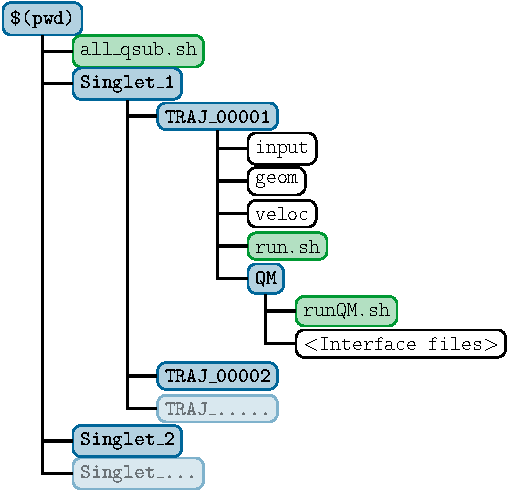
\includegraphics[scale=1]{img/dirs_traj/dirs_traj.pdf}
  \caption{Directory structure created by \ttt{setup\_traj.py}. Directories are in blue, executable scripts in green and regular files in black and white. Interface files usually include initial MO coefficients, template files and interface input files.}
  \label{fig:dirs_traj}
\end{figure}

\ttt{setup\_traj.py} will create for each initial state a directory where all trajectories starting in this state will be put. If the initial conditions file specified that the initial conditions are in the MCH representation, then the initial states will be assumed to be in the MCH representation as well. In this case, the directories will be named \ttt{Singlet\_0}, \ttt{Singlet\_1}, ..., \ttt{Doublet\_0}, \ttt{Triplet\_1}, ... If the initial states are in the diagonal representation, then the directories are simply called \ttt{X\_1}, ... since they do not have a definite spin.

In each directory, subdirectories called \ttt{TRAJ\_\%05i} are created, where \ttt{\%05i} is the initial condition index, padded to 5 digits with zeroes. In each trajectory's directory, an \sharc\ input file called \ttt{input} will be created, which contains all the dynamics options chosen during the \ttt{setup\_traj.py} run. Also, files \ttt{geom} and \ttt{veloc} will be created. For trajectories setup with \ttt{setup\_traj.py}, the determination of the initial wavefunction coefficients is done by \sharc.
Furthermore, in each trajectory directory a subdirectory \ttt{QM} is created, where the \ttt{runQM.sh} script containing the call to the interface is put. In the directory \ttt{QM} also all interface-specific input files will be copied.

For each trajectory, a \ttt{run.sh} script will be created, which can be executed to run the dynamics simulation. You might need to adapt the run script to your cluster setup.

Optionally, \ttt{setup\_traj.py} also creates a script \ttt{all\_qsub.sh}, which can be executed to submit all trajectories to a queueing system. You might need to adapt also this script to your cluster setup.

The full directory structure created by \ttt{setup\_traj.py} is given in figure~\ref{fig:dirs_traj}.



\section{Laser field generation: \ttt{laser.x}}\label{sec:laser.x}

The Fortran code \ttt{laser.x} can generate files containing laser fields which can be used with \sharc. It is possible to superimpose several lasers, use different polarizations and apply a number of chirp parameters.

\subsection{Usage}

The program is simply called by 
\begin{verbatim}
user@host> python $SHARC/laser.x
\end{verbatim}
It will interactively ask for the laser parameters. After input is complete, it writes the laser field to the file \ttt{laser} in the format which \sharc\ expects (see~\ref{sec:laserfile}).

Similar to the interactive Python scripts, \ttt{laser.x} will also write the user input to \ttt{KEYSTROKES.laser}. After modifying this file, it can be used to directly execute \ttt{laser.x} without doing the interactive input again:
\begin{verbatim}
user@host> python $SHARC/laser.x < KEYSTROKES.laser
\end{verbatim}

\subsection{Input}

The first four options are global and need to be entered only once, all remaining input options need to be given for every laser pulse. For the definition of laser fields see section~\ref{met:laser_field}.

\paragraph{Number of lasers}

Any number of lasers can be used. The output file will contain the sum of all laser pulses defined.

\paragraph{Real-valued field}

If this is true, the output file will only contain the real parts of the laser field, while the columns defining the imaginary part of the field will be zero. Note, however, that \sharc\ will anyways only use the real part of the field in the simulations.

\paragraph{Time interval and steps}

The definitions of the starting time, end time and time step of the laser field must exactly match the simulation time and time substeps of the \sharc\ simulation. Note, that the laser field must always start at $t$=0 fs to be used with \sharc. The end time for the laser field must therefore coincide with the total simulation time given in the \sharc\ input. The number of time steps for the laser field is $t_\text{total}/\Delta t_\text{sub} +1$.

\paragraph{Files for debugging}

This option is normally not needed, and can be set to False. If set to True, the chirped and unchirped laser fields in both time and frequency domain will be written to files called \ttt{DEBUG\_\dots}.

\paragraph{Polarization vector}

The polarization vector $\VEC{p}$ (will be normalized).

\paragraph{Type of envelope}

There are two options possible for the envelope function $\mathcal{E}(t)$, either a Gaussian envelope or a sinusoidal one (see~\ref{met:laser_field}).

\paragraph{Field strength}

There are two input lines for the field strength $\mathcal{E}_0$, the first defining the unit in which the field strength is defined, the second gives the corresponding number. Field strength can be read in in GV/m, TW/cm$^{-2}$ or atomic units.

\paragraph{FWHM and time intervals}

This option depends on the type of envelope chosen. While in both cases all 5 numbers need to be entered, for a Gaussian pulse only the first and third number have an effect. For a sinusoidal pulse all but the first number has an effect.

For a Gaussian pulse, the first argument corresponds to FWHM in equation~\eqref{eq:laser_gauss_2} and the third argument to $t_c$ in ~\eqref{eq:laser_gauss_1}.

For a sinusoidal pulse, the second, third, fourth and fifth argument correspond to $t_0$, $t_c$, $t_{c2}$ and $t_e$, respectively, in equation~\eqref{eq:laser_sinus}.

\paragraph{Central frequency}

There are two input lines for the central frequency $\omega_0$. The first defines the unit (wavelength in nm, energy in eV, or atomic units). The second line gives the value.

\paragraph{Phase}

The total phase $\phi$ is given in multiples of $\pi$. For example, the input ``\ttt{1.5}'' gives a phase of $\frac{3\pi}{2}$.

\paragraph{Chirp parameters}

There are four lines giving the chirp parameters $b_1$, $b_2$, $b_3$ and $b_4$. See equation~\eqref{eq:laser_chirp} for the meaning of these parameters.



\section{Calculation of Absorption Spectra: \ttt{spectrum.py}}\label{sec:spectrum.py}

Aside from setting up trajectories, the \ttt{initconds.excited} files can also be used to generate absorption spectra based on the excitation energies and oscillator strengths in the file. The script \ttt{spectrum.py} calculates Gaussian or Lorentzian convolutions of these data in order to obtain spectra. See section~\ref{met:spectrum} for further details.

\ttt{spectrum.py} evaluates the absorption spectrum on a grid for all states it finds in an initial conditions file. Using command-line options, some initial conditions can be omitted in the convolution, see table~\ref{tab:spectrum_opts}.

\subsection{Input}

The script is executed with the initial conditions file as argument:
\begin{verbatim}
user@host> python $SHARC/spectrum.py [OPTIONS] initconds.excited
\end{verbatim}

The script accepts a number of command-line options, which are given in table~\ref{tab:spectrum_opts}.
\begin{table}
  \centering
  \caption{Command-line options for script \ttt{spectrum.py}.}
  \label{tab:spectrum_opts}
  \begin{tabular}{>{\tt}lll}
    \toprule
    \rmfamily Option        &Description      &Default\\
    \midrule
    -h                  &Display help message and quit.         & --        \\
    -o FILENAME         &Output filename (for the spectrum)     &\ttt{spectrum.out}\\
    -n INTEGER          &Number of grid points                  &500       \\
    -e FLOAT FLOAT      &Energy range (eV) for the spectrum     &1 to 10 eV\\
    -i INTEGER INTEGER  &Index range for the initial conditions &1 to 1000\\
    -f FLOAT            &FWHM (eV) for the spectrum             &0.1 eV\\
    -G                  &Gaussian convolution                   &Gaussian\\
    -L                  &Lorentzian convolution                 &Gaussian\\
    -s                  &Use only selected initial conditions   &Use all\\
    -l                  &Make a line spectrum                   &Convolution\\
    -{}-gnuplot FILENAME  &Write a \textsc{Gnuplot} script        &No \textsc{Gnuplot} script\\
    \bottomrule
  \end{tabular}
\end{table}

\subsection{Output}

The script writes the absorption spectrum to a file (by default \ttt{spectrum.out}). Using the \ttt{-o} option, the user can redirect the output to a suitable file. The output is a table containing $n+2$ columns, where $n$ is the number of states found in the initial conditions file. The first column gives the energy in eV, within the given energy interval. In columns 2 to $n+1$ the state-wise absorption spectra are given. The last column contains the total absorption spectrum, i.e., the sum over all states. The table has $n_{\text{grid}}+1$ rows. For line spectra the output format is exactly the same, however, the file will contain one row for each excited state of each initial condition in the initial conditions file.

Additionally, the script writes some information about the calculation to standard output, among these the maximum of the spectrum, which can be used in order to normalize the spectrum. The reported maximum is simply the largest value in the last column of the spectrum. 

If requested, the script generates a \textsc{Gnuplot} script, which can be used to directly plot the spectrum. 






\section{File transfer: \ttt{retrieve.sh}}\label{sec:retrieve}

Usually, \sharc\ will run on some temporary directory, and not in the directory where the trajectories have been submitted from. The shell script \ttt{retrieve.sh} is a simple \ttt{scp} wrapper, which can be executed (in a directory where a trajectory has been sent from) in order to retrieve the output files of this trajectory. This might not work for every cluster setup.

It relies on the presence of the file \ttt{host\_infos}. All trajectories set up with \ttt{setup\_traj.py} create this file after the trajectory has been started with \ttt{run.sh}. \ttt{retrieve.sh} reads \ttt{host\_infos} to determine the hostname and working directory of the trajectory and then uses \ttt{scp} to retrieve the output and restart files.

The script can be called with the option ``\ttt{-lis}'' in order to only retrieve the \ttt{output.lis} file, but not the other output files.

If the script is called with the option ``\ttt{-res}'' then also the restart files and the content of the \ttt{restart/} directory are copied.

It is advisable to configure public-key authentification for the hosts running the trajectories, so that not for every execution of \ttt{retrieve.sh} a password has to be entered.











\section{Data Extractor: \ttt{data\_extractor.x}}\label{sec:data_extractor.x}

The output of \sharc\ is mainly written to \ttt{output.dat}. In order to obtain plottable files in tabular format, the Fortran program \ttt{data\_extractor.x} is used.

\subsection{Usage}

The \ttt{data\_extractor.x} is a command line tool, and is called with the \ttt{output.dat} file as an argument.
\begin{verbatim}
user@host> $SHARC/data_extractor.x output.dat
\end{verbatim}
The program will create a directory \ttt{output\_data/} in the current working directory (not necessarily in the directory where \ttt{output.dat} resides). In this directory, several files are written, containing e.g.\ the potential energies depending on time, etc.

The program will extract the complete \ttt{output.dat} file until it reaches the EOF. No further input except for the data file can be given.

\subsection{Output}

After the program finishes, the directory \ttt{output\_data/} contains a number of files. In each file, the number of columns is dependent in the total number $n$ of states $i\in\{1...n\}$. The content of the files is listed in Table~\ref{tab:outputdata}.

The file \ttt{expec.out} contains the information of \ttt{energy.out}, \ttt{spin.out} and \ttt{fosc.out} in one file. The content of \ttt{expec.out} can be conveniently plotted by using \ttt{make\_gnuscript.py} to generate a \textsc{Gnuplot} script.

\begin{table}
  \centering
  \caption{Content of the files written by \ttt{data\_extractor.x}. $n$ is the total number of states, $j$ is a state index ($j\in\{1..n\}$).}
  \label{tab:outputdata}
  \begin{tabular}{>{\tt}lcll}
    \toprule
    File  &\# Columns     &\multicolumn{2}{l}{Columns}\\
    \midrule
    coeff\_diag.out       &$2+2n$
      &$1$ &Time $t$ (fs)\\
      &&$2$ &Norm of wavefunction $\sum_j |c_j^{\text{diag}}|^2$\\
      &&$1+2j$ &$\Re (c_j^{\text{diag}})$\\
      &&$2+2j$ &$\Im (c_j^{\text{diag}})$\\
    coeff\_MCH.out       &$2+2n$
      &$1$ &Time $t$ (fs)\\
      &&$2$ &Norm of wavefunction $\sum_j |c_j^{\text{MCH}}|^2$\\
      &&$1+2j$ &$\Re (c_j^{\text{MCH}})$\\
      &&$2+2j$ &$\Im (c_j^{\text{MCH}})$\\
    energy.out       &$4+n$
      &$1$ &Time $t$ (fs)\\
      &&$2$ &Kinetic energy (eV)\\
      &&$3$ &Potential energy (eV) of active state\\
      &&$4$ &Total energy (eV)\\
      &&$4+j$ &Potential energy (eV) of state $j$\\
    fosc.out       &$2+n$
      &$1$ &Time $t$ (fs)\\
      &&$2$ &Oscillator strength of active state\\
      &&$2+j$ &Oscillator strength of state $j$\\
    spin.out       &$2+n$
      &$1$ &Time $t$ (fs)\\
      &&$2$ &Total spin expectation value of active state\\
      &&$2+j$ &Total spin expectation value of state $j$\\
    prob.out       &$2+n$
      &$1$ &Time $t$ (fs)\\
      &&$2$ &Random number from surface hopping\\
      &&$2+j$ &Cumulated hopping probability $\sum_{k=1}^j P_k$\\
    expec.out      &$4+3n$
      &$1$ &Time $t$ (fs)\\
      &&$2$ &Kinetic energy (eV)\\
      &&$3$ &Potential energy (eV) of active state\\
      &&$4$ &Total energy (eV)\\
      &&$4+j$ &Potential energy (eV) of state $j$\\
      &&$4+n+j$ &Total spin expectation value of state $j$\\
      &&$4+2n+j$ &Oscillator strength of state $j$\\
    \bottomrule
  \end{tabular}
\end{table}

\section{Plotting the Extracted Data: \ttt{make\_gnuscript.py}}\label{sec:make_gnuscript.py}

The contents of the output files of \ttt{data\_extractor.x} can be plotted with \textsc{Gnuplot}. In order to quickly generate an appropriate \textsc{Gnuplot} script, \ttt{make\_gnuscript.py} can be used. The usage is:
\begin{verbatim}
user@host> python $SHARC/make_gnuscript.py <S> [<D> [<T> [<Q> ... ] ] ]
\end{verbatim}
\ttt{make\_gnuscript.py} takes between 1 and 8 integers as command-line arguments, specifying the number of singlet, doublet, triplet, etc.\ states. It writes an appropriate \textsc{Gnuplot} script to standard out, hence redirect the output to a file, e.g.:
\begin{verbatim}
user@host> python $SHARC/make_gnuscript.py 3 0 2 > gnuscript.gp
\end{verbatim}


Then, \textsc{Gnuplot} can be run in the \ttt{output\_data} directory of a trajectory:
\begin{verbatim}
user@host> gnuplot gnuscript.gp
\end{verbatim}
This can also be accomplished in one step using a pipe, e.g.:
\begin{verbatim}
user@host> python $SHARC/make_gnuscript.py 3 0 2 | gnuplot
\end{verbatim}

The created plot script generates four different plots (press ENTER in the command-line where you started \textsc{Gnuplot} to go to the next plot). The first plot shows the potential energy of all states in the dynamics over time in the diagonal representation. The currently occupied state is marked with black circles. A thin black line gives the total energy (sum of the kinetic energy and the potential energy of the currently occupied state). Each state is colored, with one color as contour and one color at the core of the line. The contour color represents the total spin expectation value of the state. The core color represents the oscillator strength of the state with the lowest state. See figure~\ref{fig:colors} for the relevant color code.
\begin{figure}
  \centering
  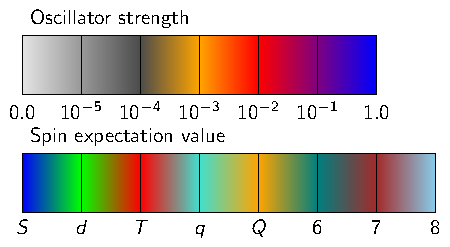
\includegraphics[scale=1]{img/colors/colors.pdf}
  \caption{Color code for plots generated with the use of \ttt{make\_gnuscript.py}.}
  \label{fig:colors}
\end{figure}
Note that by definition the ``oscillator strength'' of the lowest state with itself is exactly zero, hence the lowest state is also light grey. This dual coloring allows for a quick recognition of different types of states in the dynamics, e.g.\ singlets vs.\ triplets or $n\pi^*$ vs.\ $\pi\pi^*$ states.

The second plot shows the population $|c_i^{\text{MCH}}|^2$ of the MCH electronic states over time. The line colors are auto-generated in order to give a large spread of all colors over the excited states, but the colors might be sub-optimal, e.g.\ for printing. In this cases, the user should manually adjust the colors in the generated script.

The third plot shows the population $|c_i^{\text{diag}}|^2$ of the diagonal electronic states over time. These are the populations which are actually used for surface hopping. However, since these states are spin-mixed, it is usually difficult to interpret these populations.

The fourth plot shows the surface hopping probabilities over time. The plot is setup in such a way that the visible area corresponding to a certain state is proportional to the probability to hop into the state. Hence, if for a given timestep the random number (black circles) lies within a colored area, a surface hop to the corresponding state is performed.

\section{Calculation of Ensemble Populations: \ttt{populations.py}}\label{sec:populations.py}

For an ensemble of trajectories, usually one of the most relevant results are ensemble-averaged populations. The interactive script \ttt{populations.py} collects these populations from a set of trajectories. 

Different methods to obtain populations or quantities approximating populations can be collected, as described below.

\subsection{Usage}

The script is interactive, simply start it with no command-line arguments or options:
\begin{verbatim}
user@host> python $SHARC/populations.py
\end{verbatim}

Depending on the analysis mode (see below) it might be necessary to run \ttt{data\_extractor.x} for each trajectory prior to running \ttt{populations.py}. 

\paragraph{Paths to trajectories}

First the script asks the user to specify all directories for whose content the analysis should be performed. Enter one directory path at a time, and finish the directory input section by typing ``\ttt{end}''. Please do not specify each trajectory directory separately, but specify their parent directories, e.g.\ the directories \ttt{Singlet\_1} and \ttt{Singlet\_2}. \ttt{populations.py} will automatically include all trajectories contained in these directories.

If you want to exclude certain trajectories from the analysis, it is sufficient to create an empty file called \ttt{CRASHED} or \ttt{RUNNING} in the corresponding trajectory directory. \ttt{populations.py} will ignore all directories containing one of these files.

\paragraph{Analysis mode}

Using \ttt{populations.py}, there are two basic ways in obtaining the excited-state populations. The first way is to count the number of trajectories for which a certain condition holds. For example, the number of trajectories in each classical state can be obtained in this way. However, it is also possible to count the number of trajectories for which the total spin expectation value is within a certain interval. 
The second way to obtain populations is to obtain the sum of the absolute squares of the quantum amplitudes over all trajectories. Table~\ref{tab:Populations_modes} contains a list of all possible analysis modes.

\begin{table}
  \centering
  \caption{Analysis modes for \ttt{populations.py}. The last column indicates whether \ttt{data\_extractor.x} has to be run prior to the ensemble analysis.}
  \label{tab:Populations_modes}
  \begin{tabular}{lp{6cm}>{\tt}lc}
    \toprule
    Mode        &Description    &\rmfamily From which     &Extract?\\
                               &&\rmfamily file?          &\\
    \midrule
    1   &For each diagonal state count how many trajectories have this state as active state. &output.lis  &No\\
    2   &For each MCH state count how many trajectories have this state as approximate active state (see section~\ref{ssec:state_transform}). &output.lis  &No\\
    3   &For each MCH state count how many trajectories have this state as approximate active state (see section~\ref{ssec:state_transform}). Multiplet components are summed up. &output.lis  &No\\
    4   &Generate a histogram with definable bins (variable width). Bin the trajectories according to their total spin expectation value (of the currently active diagonal state).   &output.lis &No\\
    5   &Generate a histogram with definable bins (variable width). Bin the trajectories according to their state dipole moment expectation value (of the currently active diagonal state).   &output.lis &No\\
    6   &Generate a histogram with definable bins (variable width). Bin the trajectories according to the oscillator strength between lowest and currently active diagonal states.        &output\_data/fosc.out  &Yes\\
    7   &Calculate the sum of the absolute squares of the diagonal coefficients for each state.       &output\_data/coeff\_diag.out&Yes\\
    8   &Calculate the sum of the absolute squares of the MCH coefficients for each state.       &output\_data/coeff\_MCH.out&Yes\\
    9   &Calculate the sum of the absolute squares of the MCH coefficients for each state. Multiplet components are summed up.       &output\_data/coeff\_MCH.out&Yes\\
   10   &Calculate the sum of the absolute squares of the diabatic coefficients for each state (Only for trajectories with local diabatization).      &output\_data/coeff\_diab.out&Yes\\
    \bottomrule
  \end{tabular}
\end{table}

\paragraph{Run data extractor}

For analysis modes 6, 7, 8, 9 and 10 it is necessary to first run the data extractor (see section~\ref{sec:data_extractor.x}). This task can be accomplished by \ttt{populations.py}. However, for a large ensemble or for long trajectories this may take some time. Hence, it is not necessary to perform this step each time \ttt{populations.py} is run. 

\ttt{populations.py} will detect whether the file \ttt{output.dat} or the content of \ttt{output\_data/} is more recent. Only if \ttt{output.dat} is newer the \ttt{data\_extractor.x} will be run for this trajectory.

Note that mode 10 can only be used for trajectories using local diabatization propagation (keyword \ttt{coupling overlap} in \sharc\ input file).

\paragraph{Number of states}

For analysis modes 1, 2, 3, 7, 8 and 9 it is necessary to specify the number of states in each multiplicity. The number is auto-detected from the input file of one of the trajectories.

\paragraph{Intervals}

For analysis modes 4, 5 and 6 the user must specify the intervals for the classification of the trajectories. The user has to input a list of interval borders, e.g.:
\begin{example}
\begin{verbatim}
Please enter the interval limits, all on one line.
Interval limits: 1e-3 0.01 0.1 1
\end{verbatim}
\end{example}

Note that scientific notation can be used. Based on this input, for each timestep a histogram is created with the number of trajectories in each interval. The histogram bins are:
\begin{enumerate}
  \item $x\leq10^{-3}$
  \item $10^{-3}<x\leq10^{-2}$
  \item $10^{-2}<x\leq10^{-1}$
  \item $10^{-2}<x\leq10^{0}$
  \item $10^{0}<x$
\end{enumerate}
Note that there is always one more bin that interval borders entered.

\paragraph{Normalization}

If desired, \ttt{populations.py} can normalize the populations by dividing the populations by the number of trajectories. 

\paragraph{Maximum simulation time}

This gives the maximum simulation time until which the populations are analyzed. For trajectories which are shorter than this value, the last population information is used to make the trajectory long enough. Trajectories which are longer are not analyzed to the end. \ttt{populations.py} prints the length of the shortest and longest trajectories after the analysis.

\paragraph{Gnuplot script}

\ttt{populations.py} can generate an appropriate \textsc{Gnuplot} script for the performed population analysis. 

\subsection{Output}

By default, \ttt{populations.py} writes the resulting populations to \ttt{pop.out}. If the file already exists, the user is ask whether it shall be overwritten, or to provide an alternative filename. Note that the output file is checked only after the analysis is completed, so the program might run for a considerable amount of time before asking for the output file.


\section{Obtaining special geometries: \ttt{crossing.py}}\label{sec:crossing.py}

In many cases, it is also important to obtain certain special geometries from the trajectories. The script \ttt{crossing.py} extracts geometries fulfilling special conditions from an ensemble of trajectories. 

Currently, \ttt{crossing.py} finds geometries where the approximate MCH state (see section~\ref{ssec:state_transform}) of the last timestep is different from the MCH state of the current timestep (i.e.\ \ttt{crossing.py} finds geometries where surface hops occured). 

\subsection{Usage}

The script is interactive, simply start it with no command-line arguments or options:
\begin{verbatim}
user@host> python $SHARC/crossing.py
\end{verbatim}

The input to the script is very similar to the one of \ttt{populations.py}. 

\paragraph{Paths to trajectories}

First the script asks the user to specify all directories for whose content the analysis should be performed. Enter one directory path at a time, and finish the directory input section by typing ``\ttt{end}''. Please do not specify each trajectory directory separately, but specify their parent directories, e.g.\ the directories \ttt{Singlet\_1} and \ttt{Singlet\_2}. \ttt{crossing.py} will automatically include all trajectories contained in these directories.

If you want to exclude certain trajectories from the analysis, it is sufficient to create an empty file called \ttt{CRASHED} or \ttt{RUNNING} in the corresponding trajectory directory. \ttt{crossing.py} will ignore all directories containing one of these files.

\paragraph{Analysis mode}

Currently, \ttt{crossing.py} only supports one analysis mode, where \ttt{crossing.py} is scanning for each trajectory the file \ttt{output.lis}. If the occupied MCH state (column 4 in output file \ttt{output.lis}) changes from one timestep to the next, it is checked whether the old and new MCH states are the ones specified by the user. If this is the case, the geometry corresponding to the new timestep ($t$) is retrieved from \ttt{output.xyz} (lines $t(n_{\text{atom}}+2)+1$ to $t(n_{\text{atom}}+2)+n_{\text{atom}}$). 

\paragraph{States involved in surface hop}

First, the user has to specify the permissible old MCH state. The state has to be specified with two integers, the first giving the multiplicity (\ttt{1}=singlet, ...), the second the state within the multiplicity (\ttt{1 1}=$S_0$, \ttt{1 2}=$S_1$, etc.). If a state of higher multiplicity is given, \ttt{crossing.py} will report all geometries where the old MCH state is any of the multiplet components. 

For the new MCH state, the same is valid.

Third, the direction of the surface hop has to be specified. Choosing ``Backwards'' has the same effect as exchanging the old and new MCH states. 

\subsection{Output}

All geometries are in the end written to an output file, by default \ttt{crossing.xyz}. The file is in standard xyz format. The comment of each geometry gives the path to the trajectory where this geometry was extracted, the simulation time and the diagonal and MCH states at this simulation time. 





\section{Internal Coordinates Analysis: \ttt{geo.py}}\label{sec:geo.py}

\sharc\ writes at every timestep the molecular geometry to the file \ttt{output.xyz}. The non-interactive script \ttt{geo.py} can be used in order to extract internal coordinates from xyz files. The usage is:
\begin{verbatim}
user@host> python $SHARC/geo.py [options] < Geo.inp > Geo.out
\end{verbatim}
By default, the coordinates are read from \ttt{output.xyz}, but this can be changed with the \ttt{-g} option (see table~\ref{tab:Geo_options}). Note that the internal coordinate specifications are read from standard input and the result table is written to standard out. 

\subsection{Input}

The specifications for the desired internal coordinates are read from standard input. It follows a simple syntax, where each internal coordinate is specified by a single line of input. Each line starts with a one-letter key which specifies the type of internal coordinate (e.g.\ bond length, angle, dihedral, ...). The key is followed by a list of integers, specifying which atoms should be measured. As a simple example, \ttt{r 1 2} specifies the bond length (\ttt{r} is the key for bond lengths) between atoms 1 and 2. Note that the numbering of the atoms starts with 1. Each line of input is checked for consistency (whether any atom index is larger than the number of atoms, repeated atom indices, misspelled keys, wrong number of atom indices, ...), and erroneous lines are ignored (this is indicate by an error message).

Table~\ref{tab:Geo_input} lists the available types of internal coordinates. The output is a table, where the first column is the time (Actually, the geometries are just enumerated starting with zero, and the number multiplied by the timestep from the \ttt{-t} option). The successive columns in the output table list the results of the internal coordinates calculations. Each request generates at least one column, see table~\ref{tab:Geo_input}. 

Note that for most internal coordinates, the order of the atoms is crucial, since e.g.\ $a_{123}\neq a_{213}$. This also holds for the Cremer-Pople parameter requests. For these input lines, the atoms should be listed in the order they appear in the ring (clockwise or counter-clockwise).

\begin{table}[h]
  \centering
  \caption{Possible types of internal coordinates in \ttt{geo.py}. }
  \label{tab:Geo_input}
  \begin{tabular}{>{\tt}c>{\bfseries\ttfamily}lll}
    \toprule
    \rmfamily Key         &\normalfont\rmfamily Atom      &Description    &Output columns\\
                          &\normalfont\rmfamily Indices   &               &\\
    \midrule
    x   &a              &$x$ coordinate of atom \ttt{a}         &$x$\\
    y   &a              &$y$ coordinate of atom \ttt{a}         &$y$\\
    z   &a              &$z$ coordinate of atom \ttt{a}         &$z$\\
    r   &a b            &Bond length between \ttt{a} and \ttt{b}        &$r$\\
    a   &a b c          &Angle between \ttt{a}--\ttt{b} and \ttt{b}--\ttt{c}         &$a$\\
    d   &a b c d        &Dihedral (Angle between planes (\ttt{a,b,c})    &$d$\\
                       &&and (\ttt{b,c,d}))&\\
    p   &a b c d        &Pyramidalization angle (90$^\circ$ minus angle    &$p$\\
                       &&between bond \ttt{a}--\ttt{b} and plane (\ttt{b,c,d}))&\\
    5   &a b c d e      &Cremer-Pople parameters for 5-membered&$q_2$, $\phi_2$\\
                       &&rings \cite{Cremer1975JACS}.&\\
    6   &a b c d e f    &Cremer-Pople parameters for 6-membered&$Q$, $\phi$, $\theta$, Boeyens\\
                       &&rings \cite{Cremer1975JACS} and Boeyens classification \cite{Boeyens1976JCMS}.&\\
    c   &               &Writes the comment (second line of the &Comment\\
                       &&xyz format) to the table.&\\
    \bottomrule
  \end{tabular}
\end{table}

As an advice, it is always a good idea to put the comment as the \textit{last} request, if at all. Since the comment may contain blanks, having the comment not as the very last column might make it impossible to plot the resulting table.

The Boeyens classification symbols which are output for 6-membered rings are reported in \LaTeX\ math code. Note that in the Boeyens classification scheme a number of symbols are equivalent, and only one symbol is reported. For example, by definition the chair configuration $^1C_4$ is equivalent to $^5C_2$ and $^3C_6$.

\subsection{Options}

\ttt{geo.py} accepts a number of command-line options, see table~\ref{tab:Geo_options}. All options have sensible defaults. However, especially if long comments should be written to the output file, it might be necessary to increase the field width. Note that the minimum column width is 20 so that the table header can be printed correctly.

\begin{table}[h]
  \centering
  \caption{Command-line options for \ttt{geo.py}. }
  \label{tab:Geo_options}
  \begin{tabular}{>{\tt}lll}
    \toprule
    \rmfamily Option         &Description    &Default\\
    \midrule
    -h          &Display help message and quit.         & --        \\
    -b          &Report $x$, $y$, $z$, $r$, $q_2$ and $Q$ in Bohrs       &Angstrom\\
    -r          &Report $a$, $d$, $p$, $\phi_2$, $\phi$ and $\theta$ in Radians         &Degrees\\
    -g FILENAME &Read coordinates from the specified file       &\ttt{output.xyz}\\
    -t FLOAT    &Assumed timestep between successive geometries (fs)    &1.0 fs\\
    -p INTEGER  &Precision (Number of decimals, max.~width--3)         &4\\
    -w INTEGER  &Width of each column (min.~20)                   &20\\
    \bottomrule
  \end{tabular}
\end{table}








\section{Diagonalization Helper: \ttt{diagonalizer.x}}\label{sec:diagonalizer.x}

The small program \ttt{diagonalizer.x} is used by the Python scripts to diagonalize matrices if the \textsc{NumPy} library is not available. Currently, only \ttt{excite.py} and \ttt{SHARC\_Analytical.py} need to diagonalize matrices. The program \ttt{diagonalizer.x} is implemented as a simple front-end to the LAPACK libary.

The program reads from stdin. The first line consists of the letter ``r'' or ``c'', followed by two integers giving the matrix dimensions. For ``r'', the program assumes a real symmetric matrix, for ``c'' a Hermitian matrix. The matrix must be square.
The second line is a comment and is ignored.
In the following lines, the matrix elements are given. On each line one row of the matrix has to be written. If the matrix is complex, each line contains the double number of entries, where real and imaginary part are always given subsequently.
The following is an example input:
\begin{example}
\footnotesize\begin{verbatim}
c 2 2
comment
1.0  0.0    2.0  0.1
2.0 -0.1    6.0  0.0
\end{verbatim}
\end{example}

\normalsize
for the matrix 
\begin{equation}
  A=\begin{pmatrix}
      1 &2+0.1i\\
      2-0.1i&6
    \end{pmatrix}.\nonumber
\end{equation}
The diagonal matrix and the matrix of eigenvectors is written to stdout.



% ========================================================================================================= %
% ========================================================================================================= %
% ========================================================================================================= %

\chapter{Methodology}

In this chapter different aspects of \sharc\ simulations are discussed in detail. The topics are ordered alphabetically.


\section{Absorption Spectrum}\label{met:spectrum}

Using \ttt{spectrum.py}, an absorption spectrum can be calculated as the sum over the absorption spectra of each individual initial condition:
\begin{equation}
  \sigma(E)=\sum\limits_i^{n_\text{init}} \sigma_i(E),
\end{equation}
where $i$ runs over the initial conditions.

The spectrum of a single initial condition is the convolution of its line spectrum, defined through a set of tuples $(E^\alpha,f_\text{osc}^\alpha)$ for each electronic state $\alpha$, where $E^\alpha$ is the excitation energy and $f_\text{osc}^\alpha)$ is the oscillator strength.

The convolution of the line spectrum can be performed with \ttt{spectrum.py} using either Gaussian or Lorentzian functions. The contribution of a state $\alpha$ to the absorption spectrum $\sigma^\alpha(E)$ is given by:
\begin{align}
  \sigma_{\text{Gaussian}}^\alpha(E)&=
  \left(f_{\text{osc}}\right)_i^\alpha 
  \E^{c\left(E-E_i^\alpha\right)^2},\\
  \text{with}\qquad
  c&=-\frac{4\ln(2)}{\text{FWHM}^2},
\end{align}
or
\begin{align}
  \sigma_{\text{Lorentzian}}^\alpha(E)&=
  \frac{\left(f_{\text{osc}}\right)_i^\alpha}{\frac{1}{c}\left(E-E_i^\alpha\right)^2+1},\\
  \text{with}\qquad
  c&=\frac{1}{4}\text{FWHM}^2,
\end{align}
where FWHM is the full width at half maximum.


\section{Active and inactive states}\label{met:activestates}

\sharc\ allows to ``freeze'' certain states, which then do not participate in the dynamics. Only energies and dipole moments are calculated, but all couplings are disabled. In this way, these states are never visited (hence also no gradients and non-adiabatic couplings are calculated, making the inclusion of these states cheap). Example:

\newcommand{\R}{\cellcolor{RL!30}}
\begin{example}
  \verb|nstates 2 0 2|

  \verb|actstates 2 0 1|
\end{example}

In the example given, state $T_2$ is frozen. The corresponding Hamiltonian looks like:

\begin{equation}
  \VEC{H}=
  \begin{pmatrix}
&      E(S_0)    &             &   a^*_{01} &\R a^*_{02}   &   b^*_{01} &\R b^*_{02}   &a_{01}       &\R a_{02}&\\
&                &   E(S_1)    &   a^*_{11} &\R a^*_{12}   &   b^*_{11} &\R b^*_{12}   &a_{11}       &\R a_{12}&\\
&      a_{01}    &   a_{11}    &   E(T_1)   &\R p^*_{12}   &            &\R{-q^*_{12}} &             &\R&\\
&  \R a_{02}    &\R a_{12}    &\R p_{12}   &   E(T_2)     &\R q^*_{12} &\R            &\R           &\R&\\
&      b_{01}    &   b_{11}    &            &\R -q_{12}    &   E(T_1)   &\R            &             &\R -q^*_{12}&\\
&  \R b_{02}    &\R b_{12}    &\R q_{12}   &\R            &\R          &   E(T_2)     &\R q^*_{12}  &\R&\\
&      a^*_{01}  &   a^*_{11}  &            &\R            &            &\R -q_{12}    &   E(T_1)    &\R p_{12}&\\
&  \R a^*_{02}  &\R a^*_{12}  &\R          &\R            &\R q_{12}   &\R            &\R p^*_{12}  &   E(T_2)&\\
  \end{pmatrix}\nonumber
\end{equation}
where all matrix elements marked \begin{tabular}{c}\cellcolor{RL!50}red\end{tabular} are deleted, since $T_2$ is frozen. 

The corresponding matrix elements are also deleted from the non-adiabatic coupling and overlap matrices. For propagation including laser fields, also the corresponding transition dipole moments are neglected, while the transition dipole moments still show up in the output (in order to characterize the frozen states).

Active and frozen states are defined with the \ttt{states} and \ttt{actstates} keywords in the input file. Note that only the highest states in each multiplicity can be frozen, i.e., it is not possible to freeze the $T_1$ while having $T_2$ active. However, it is possible to freeze all states of a certain multiplicity.


\section{Damping}\label{met:damping}

If damping is activated in \sharc\ (keyword \ttt{dampeddyn}), in each timestep the following modification to the velocity vector is made
\begin{equation}
  \VEC{v}^\prime=\VEC{v}\cdot\sqrt{C}
\end{equation}
where $C$ is the damping factor given in the input. Hence, in each timestep the kinetic energy is modified by
\begin{equation}
  E_{\text{kin}}^\prime=E_{\text{kin}}\cdot C
\end{equation}
The damping factor $C$ must be between 0 and 1.


\section{Decoherence}\label{met:decoherence}

In surface hopping, without any corrections the coherence between the states is usually too large \cite{Granucci2007JCP}. A trajectory in state $\beta$, but where state $\alpha$ has a large coefficient, will still travel according to the gradient of state $\beta$. However, the gradients of state $\alpha$ are almost certainly different to the ones of state $\beta$. As a consequence, too much population of state $\alpha$ is following the gradient of state $\beta$. Decoherence corrections damp in different ways the population of all states $\alpha\neq\beta$, so that only population of $\beta$ follows the gradient of state $\beta$.

The decoherence correction currently implemented in \sharc\ is based on the energies of the excited states (``energy-based decoherence'', or EDC, as given in \cite{Granucci2010JCP}). After the surface hopping procedure, when the system is in state $\beta$, the coefficients are updated by the following relation
\begin{align}
  c_\alpha^\prime=&
  c_\alpha\cdot\exp
  \left[
    -\Delta t\frac{|E_\alpha-E_\beta|}{\hbar}
    \left(
      1+\frac{C}{E_{\text{kin}}}
    \right)^{-1}
  \right],\qquad \alpha\neq\beta,\\
  c_\beta^\prime=&
  \frac{c_\beta}{|c_\beta|}\cdot
  \left[
    1-\sum\limits_{\alpha\neq\beta}^{\vphantom{\alpha}} |c^\prime_\alpha|^2
  \right]^{\frac{1}{2}}
\end{align}
where $C$ is the decoherence parameter. The decoherence correction can be activated with the keyword \ttt{decoherence} in the input file. The decoherence parameter $C$ can be set with the keyword \ttt{decoherence\_param} (the default is 0.1~hartree, as suggested in \cite{Granucci2010JCP}).


\section{Excitation Selection}\label{met:exc_selection}

\ttt{excite.py} can select initial active states for the dynamics based on for each initial condition $k$ the excitation energies $E_{k,\alpha}$ and the oscillator strengths $f^{\text{osc}}_{k,\alpha}$ are known for the excited states $\alpha$. The procedure is based on reference~\cite{Barbatti2011}.

First, for all excited states of all initial conditions, the maximum value $p_{\text{max}}$ of 
\begin{equation}
  p_{k,\alpha}=\frac{f^{\text{osc}}_{k,\alpha}}{E_{k,\alpha}^2} \label{eq:exc_prob}
\end{equation}
is found. Then for each excited state, a random number $r_{k,\alpha}$ is picked from $[0,1]$. If
\begin{equation}
  r_{k,\alpha}<\frac{p_{k,\alpha}}{p_{\text{max}}}
\end{equation}
then the excited state is selected for performing the dynamics. This excited-state selection scheme is taken from \cite{Barbatti2011}.

Within \ttt{excite.py} it is possible to restrict the selection to a subset of all excited states. In this case, also $p_{\text{max}}$ is only determined based on this subset of excited states.


% \section{Gradient transformation}\label{met:gradtra}
% 
% Since the actual dynamics is performed on the PESs of the diagonal states, also the gradients have to be transformed to the diagonal representation. To this end, first a generalized gradient matrix $\VEC{G}^{\text{MCH}}$ is constructed from the gradients %
% %%tth: $\VEC{g}^{\text{MCH}}_\alpha=-\nabla_RH_{\alpha\alpha}^{\text{MCH}}$
% \tthdump{%
% $\VEC{g}^{\text{MCH}}_\alpha=-\nabla_\VEC{R}H_{\alpha\alpha}^{\text{MCH}}$%
% }
% and the non-adiabatic coupling vectors 
% $\VEC{K}_{\beta\alpha}^{\text{MCH}}$:
% \begin{equation}
%   \VEC{G}^{\text{MCH}}=
%   \begin{pmatrix}
%     \VEC{g}_1   &-(H_{11}-H_{22})\VEC{K}_{12} &-(H_{11}-H_{33})\VEC{K}_{13} &\cdots\\
%     -(H_{22}-H_{11})\VEC{K}_{21}      &\VEC{g}_2      &-(H_{22}-H_{33})\VEC{K}_{23}&\cdots\\
%     -(H_{33}-H_{11})\VEC{K}_{31}      &-(H_{33}-H_{22})\VEC{K}_{32} &\VEC{g}_3\\
%     \vdots      &\vdots         &       &\ddots
%   \end{pmatrix}
% \end{equation}
% Note that all quantities in the matrix are in the MCH representation, the superscripts were omitted for brevity.
% 
% The matrix $\VEC{G}^{\text{MCH}}$ is subsequently transformed into the diagonal representation, using the transformation matrix $\VEC{U}$:
% \begin{equation}
%   \VEC{G}^{\text{diag}}=\VEC{U}^\dagger\VEC{G}^{\text{MCH}}\VEC{U}.
% \end{equation}
% The diagonal elements of $\VEC{G}^{\text{diag}}$ now contain the gradients of the diagonal states, while the off-diagonal elements contain the scaled non-adiabatic couplings $-(H^{\text{diag}}_{\beta\beta}-H^{\text{diag}}_{\alpha\alpha})\VEC{K}_{\beta\alpha}^{\text{diag}}$. The gradients are needed in the Velocity Verlet algorithm in order to propagate the nuclear coordinates. The non-adiabatic couplings are necessary if the velocity vector is to be rescaled along the non-adiabatic coupling vector.
% 
% Since the matrix $\VEC{G}^{\text{MCH}}$ contains elements which are itself vectors with $3N$ components, the transformation is done component-wise (e.g.\ first a matrix $G_{x,\text{atom} 1}$ is constructed from the $x$ components of all gradients (and non-adiabatic couplings) for atom $1$, this matrix is transformed and written to the $x$, atom $1$ component of $\VEC{G}^{\text{diag}}$, then this is repeated for all components).
% 
% Since the calculation of the non-adiabatic couplings $\VEC{K}^{\text{MCH}}_{\beta\alpha}$ might add considerable computational cost, there is the input keyword \ttt{nogradcorrect} which tells \sharc\ to neglect the $\VEC{K}^{\text{MCH}}_{\beta\alpha}$ in the gradient transformation.
% 
% \subsection{Dipole moment derivatives}\label{met:dipolegrad}
% 
% For strong laser fields, the derivative of the dipole moments might be a non-negligible contribution to the gradients. In this case, they should be included in the gradient transformation step:
% \begin{equation}
%   \VEC{G}^{\text{diag}}=\VEC{U}^\dagger
%   \left[
%     \VEC{G}^{\text{MCH}}
%     -\boldsymbol{\epsilon}(t)\cdot\frac{\partial}{\partial R}\boldsymbol{\mu}
%   \right]\VEC{U}.
% \end{equation}
% This can be activated with the keyword \ttt{dipole\_grad} in the \sharc\ input file.


\section{Internal coordinates definitions}\label{met:geo}

In this section, the internal coordinates available in \ttt{geo.py} are defined.

\paragraph{Bond length}

The bond length between two atoms $a$ and $b$ is:
\begin{equation}
  r_{ab}=
  \sqrt{
    (x_a-x_b)^2+(y_a-y_b)^2+(z_a-z_b)^2
  }
\end{equation}

\paragraph{Bond angle}

The bond angle for atoms $a$, $b$ and $c$ is defined as the angle
\begin{equation}
  \theta=
  \cos^{-1}\left(
    \frac{\VEC{v}_{ba}\cdot\VEC{v}_{bc}}{|\VEC{v}_{ba}|\cdot|\VEC{v}_{bc}|}
  \right)\label{eq:angle}
\end{equation}
where $\VEC{v}_{ba}$ is the vector from atom $b$ to atom $a$.

\paragraph{Dihedral}

The dihedral angle is defined via the vectors $\VEC{w}_1$ and $\VEC{w}_2$:
\begin{equation}
  \VEC{w}_1=\VEC{v}_{ab}\times\VEC{v}_{bc}\qquad\text{and}\qquad\VEC{w}_1=\VEC{v}_{ab}\times\VEC{v}_{bc}.
\end{equation}
The dihedral is given as the angle between $\VEC{w}_1$ and $\VEC{w}_2$ according to equation~\eqref{eq:angle}.

\paragraph{Pyramidalization angle}

The pyramidalization angle is defined via the vectors $\VEC{v}_{ba}$ and 
\begin{equation}
  \VEC{w}_1=\VEC{v}_{bc}\times\VEC{v}_{bd}.
\end{equation}
The pyramidalization angle is then given as $90^\circ - \theta(\VEC{v}_{ba},\VEC{w}_1)$.

\paragraph{Cremer-Pople parameters}

The definitions of the Cremer-Pople parameters for 5- and 6-membered rings is described in \cite{Cremer1975JACS}.

\paragraph{Boeyens classification}

The Boeyens classification scheme is described in \cite{Boeyens1976JCMS}.

\section{Kinetic energy adjustments}\label{met:ekinadj}

There are several options how to adjust the kinetic energy after a surface hop occured. The simplest option is to not adjust the kinetic energy at all (input: \ttt{ekincorrect none}), but this obviously leads to violation of the conservation of total energy.

Alternatively, the velocities of all atoms can be rescaled so that the new kinetic energy and the potential energy of the new state $\beta$ again sum up to the total energy.
\begin{align}
  f&=\sqrt{\frac{E_{\text{total}}-E_\beta}{E_{\text{kin}}}}\\
  \VEC{v}^\prime&=f\VEC{v}\\
  E_{\text{kin}}^\prime&=f^2E_{\text{kin}}
\end{align}
Within this methodology, when the energy of the old state $\alpha$ was lower than the energy of the new state $\beta$ the kinetic energy is lowered. Since the kinetic energy must be positive, this implies that there might be states which cannot be reached (their potential energy is above the total energy). A hop to such a state is called ``frustrated hop'' and will be rejected by \sharc. Rescaling parallel to the nuclear velocity vector is requested with \ttt{ekincorrect parallel\_vel}.

Alternatively, according to Tully's original formulation of the surface hopping method \cite{Tully1990JCP}, after a hop from $\alpha$ to $\beta$ only the component of the velocity along the direction of the non-adiabatic coupling vector $\VEC{K}_{\beta\alpha}$ should be rescaled. With
\begin{align}
  a&=\sum\limits_i^{N_\mathrm{atom}} \frac{\VEC{K}_{\beta\alpha, i}\cdot\VEC{K}_{\beta\alpha, i}}{2M_i}\\
  b&=\sum\limits_i^{N_\mathrm{atom}} \VEC{v}_{i}\cdot\VEC{K}_{\beta\alpha, i}
\end{align}
the available energy can be calculated:
\begin{equation}
  \Delta=
  4a
  \left(
    E_\alpha-E_\beta
  \right)+b^2.
\end{equation}
If $\Delta<0$, the hop is frustrated and will be rejected. Otherwise, the scaled velocities $\VEC{v}^\prime$ can be calculated as
\begin{align}
  \VEC{v}_i^\prime&=\VEC{v}_i-f\frac{\VEC{K}_{\beta\alpha, i}}{M_i}\\
  \mathrm{with}\quad f&=
  \begin{cases}
    \frac{b+\sqrt{\Delta}}{2a},\qquad b<0,\\
    \frac{b-\sqrt{\Delta}}{2a},\qquad b\geq 0.
  \end{cases}
\end{align}
This procedure can be requested with \ttt{ekincorrect parallel\_nac}. Note that in this case \sharc\ will request the non-adiabatic coupling vectors, even if they are not used for the wavefunction propagation.


\section{Laser fields}\label{met:laser_field}

The program \ttt{laser.x} can calculate laser fields as superpositions of several analytical, possibly chirped, laser pulses. In the following, the laser parametrization is given (see \cite{Marquetand2007} for further details).

\subsection{Form of the laser field}

In general, the laser field $\boldsymbol{\epsilon}(t)$ is a linear superposition of a number of laser pulses $l_i(t)$:
\begin{equation}
  \boldsymbol{\epsilon}(t)=\sum\limits_i \VEC{p}_il_i(t),
\end{equation}
where $\VEC{p}_i$ is the normalized polarization vector of pulse $i$.

A pulse $l(t)$ is formed as the product of an envelope function and a field function. 
\begin{equation}
  l(t)=\mathcal{E}(t)f(t)
\end{equation}

\subsection{Envelope functions}

There are two types of envelope function defined in \ttt{laser.x}, which are Gaussian and sinusoidal.

The Gaussian envelope is defined as:
\begin{align}
  \mathcal{E}(t)&=\mathcal{E}_0 \E^{-\beta(t-t_c)^2}\label{eq:laser_gauss_1}\\
  \beta&=\frac{4\ln 2}{\mathrm{FWHM}^2}\label{eq:laser_gauss_2}
\end{align}
where $\mathcal{E}_0$ is the peak field strength, FWHM is the full width at half maximum and $t_c$ is the temporal center of the pulse.

The sinusoidal envelope is defined as:
\begin{equation}
  \mathcal{E}(t)=\mathcal{E}_0
  \begin{cases}
    0                                                   &\text{if } t<t_0,\\
    \sin^2\left(\frac{\pi(t-t_0)}{2(t_c-t_0)}\right)      &\text{if } t_0<t<t_c,\\
    1                                                   &\text{if } t_c<t<t_{c2},\\
    \cos^2\left(\frac{\pi(t-t_{c2})}{2(t_e-t_{c2})}\right)      &\text{if } t_{c2}<t<t_e,\\
    0                                                   &\text{if } t_e<t,\label{eq:laser_sinus}
  \end{cases}
\end{equation}
where again $\mathcal{E}_0$ is the peak field strength, $t_0$ and $t_c$ define the interval where the field strength increases, and $t_{c2}$ and $t_e$ define the interval where the field strength decreases. Figure~\ref{fig:laser_envelope} shows the general form of the envelope functions and the meaning of the temporal parameters $t_0$, $t_c$, $t_{2c}$ and $t_e$.

\begin{figure}[h!]
  \centering
  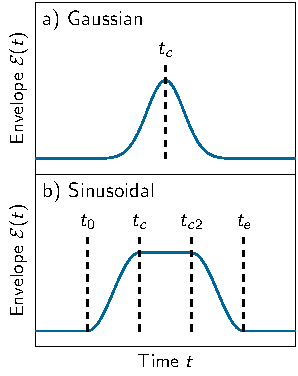
\includegraphics[scale=1]{img/laser_envelope/laser_envelope.pdf}
  \caption{Types of laser envelopes implemented in \ttt{laser.x}.}
  \label{fig:laser_envelope}
\end{figure}

\subsection{Field functions}

The field function $f(t)$ is defined as:
\begin{equation}
  f(t)=\E^{\I \left(\omega_0(t-t_c)+\phi\right)},
\end{equation}
where $\omega_0$ is the central frequency and $\phi$ is the phase of the pulse. Even though the laser field is complex in this expression, in the propagation of the electronic wavefunction in \sharc\ only the real part is used.

\subsection{Chirped pulses}

In order to apply a chirp to the laser pulse $l(t)$, it is first Fourier transformed to the frequency domain, giving the function $\tilde{l}(\omega)$. The chirp is applied by calculating:
\begin{equation}
  \tilde{l}^\prime(\omega)=
  \tilde{l}(\omega)
  \E^{-i\left[
  b_1|\omega-\omega_0|
  +\frac{b_2}{2}(\omega-\omega_0)^2
  +\frac{b_3}{6}(\omega-\omega_0)^3
  +\frac{b_4}{24}(\omega-\omega_0)^4
  \right]}\label{eq:laser_chirp}
\end{equation}
The chirped laser in the time domain $l^\prime(t)$ is then obtained by Fourier transform of the chirped pulse $\tilde{l}^\prime(\omega)$.


\subsection{Quadratic chirp without Fourier transform}

If \ttt{laser.x} was compiled without the FFTW package, the only accessible chirps are quadratic chirps for Gaussian pulses:
\begin{align}
  l(t)=&
  \mathcal{E}_0^\prime
  \E^{-\beta^\prime(t-t_c)^2}
  \E^{-\I\left(
    \omega_0(t-t_c)+a_2(t-t_c)^2+\phi
  \right)}\\
  \beta=&\frac{4\ln 2}{\mathrm{FWHM}^2}\\
  \beta^\prime=&\frac{1}{\frac{1}{\beta}+4\beta b_2^2}\\
  a_2=&\frac{b_2}{\frac{1}{4\beta^2}+b^2_2}\\
  \mathcal{E}_0^\prime=&\mathcal{E}_0\sqrt{\frac{1}{2\I b_2\beta+1}}
\end{align}
Other chirps are only possible with the Fourier transformation.


\section{Laser interactions}\label{met:laser}

The laser field $\boldsymbol{\epsilon}$ is included in the propagation of the electronic wavefunction. In each substep of the propagation, the interaction of the laser field with the dipole moments is included in the Hamiltonian. The contribution $\VEC{V}_i$ is in each timestep added to the Hamiltonian in equations~\eqref{eq:ham_propn} or \eqref{eq:ham_propl}, respectively:
\begin{align}
  \VEC{V}_i=&
  -
  \Re\left(
    \boldsymbol{\mu}_i\cdot
    \boldsymbol{\epsilon}_i
  \right),\\
  \boldsymbol{\mu}_i=&
  \boldsymbol{\mu}^{\text{MCH}}(t) + \frac{i}{n}
  \left(
    \boldsymbol{\mu}^{\text{MCH}}(t+\Delta t)-\boldsymbol{\mu}^{\text{MCH}}(t)
  \right),\\
  \boldsymbol{\epsilon}_i=&\boldsymbol{\epsilon}\left(t+\frac{i}{n}\Delta t\right)
\end{align}
where $i$, $n$ $t$ and $\Delta t$ are defined as in section \ref{met:propagate}.

\subsection{Surface Hopping with laser fields}

If laser fields are present, there can be two fundamentally different types of hops: laser-induced hops and non-adiabatic hops. The latter ones are the same hops as in the laser-free simulations, and demand that the total energy is conserved. The laser-induced hops on the other hand demand that the momentum (kinetic energy) is conserved. Hence, \sharc\ needs to decide for every hop whether it is laser-induced or not. 

Consider a previous state $\alpha$ and a new state $\beta$. Currently, the hop is classified based on the energy gap $\Delta E=|E_\beta^\text{diag}-E_\alpha^\text{diag}|$ and the instantaneous central energy of the laser pulse $\omega$. 
The hop is assumed to be laser-induced if
\begin{equation}
  |\Delta E-\omega| < W,
\end{equation}
where $W$ is a fixed parameter. $W$ can be set using the input keyword \ttt{laserwidth}.

If a hop has been classified as laser-free, the momentum is adjusted according to the equations given in section~\ref{met:ekinadj}.

% \section{Phase tracking}
% 
% \subsection{Phase tracking of the transformation matrix}\label{met:phase_track}
% 
% A Hermitian matrix $\VEC{H}^{\text{MCH}}$ can always be diagonalized. Its eigenvectors form the rows of a unitary matrix $\VEC{U}$, which can be used to transform between the original basis and the basis of the eigenfunctions of $\VEC{H}$. 
% \begin{equation}
%   \VEC{H}^{\text{diag}}=\VEC{U}^\dagger\VEC{H}^{\text{MCH}}\VEC{U}.
% \end{equation}
% 
% However, the condition that $\VEC{U}$ diagonalizes $\VEC{H}^{\text{MCH}}$ is not sufficient to define $\VEC{U}$ uniquely. Each normalized eigenvector $\VEC{u}$ can be multiplied by a complex number on the unit circle and still remains a normalized eigenvector:
% \begin{align}
%   \VEC{H}\VEC{u}=h\VEC{u}
%   \qquad&\text{and}\qquad
%   \VEC{u}^\dagger\VEC{u}=1\\
%   &\Rightarrow\nonumber\\
%   \VEC{H}\left(\E^{\I\phi}\VEC{u}\right)
%   =\E^{\I\phi}\left(\VEC{H}\VEC{u}\right)
%   &=\E^{\I\phi}h\VEC{u}
%   =h\left(\E^{\I\phi}\VEC{u}\right)\\
%   &\text{and}\nonumber\\
%   \left(\E^{\I\phi}\VEC{u}\right)^\dagger\left(\E^{\I\phi}\VEC{u}\right)
%   =\VEC{u}^\dagger\E^{-\I\phi}&\E^{\I\phi}\VEC{u}
%   =\VEC{u}^\dagger\VEC{u}=1
% \end{align}
% Thus, for all diagonal matrices $\boldsymbol{\Phi}$ with elements 
% %%tth: $\delta_{\beta\alpha}\exp(\I\phi_\beta)$, 
% \tthdump{
%   $\delta_{\beta\alpha}\E^{\I\phi_\beta}$, 
% }
% also the matrix $\VEC{U}^\prime=\VEC{U}\boldsymbol{\Phi}$ diagonalizes $\VEC{H}^{\text{MCH}}$ (if $\VEC{U}$ diagonalizes it).
% 
% The propagation of the coefficients in the diagonal basis is written as (see section~\ref{met:propagate}):
% \begin{equation}
%   \VEC{c}^{\text{diag}}(t+\Delta t)=\underbrace{\VEC{U}^\dagger(t+\Delta t)\VEC{R}^{\text{MCH}}(t+\Delta t,t)\VEC{U}(t)}_{\VEC{R}^{\text{diag}}(t+\Delta t,t)}\VEC{c}^{\text{diag}}(t)
% \end{equation}
% where $\VEC{U}(t)$ and $\VEC{U}(t+\Delta t)$ are determined independently from diagonalizing the matrices $\VEC{H}^{\text{MCH}}(t)$ and $\VEC{H}^{\text{MCH}}(t+\Delta t)$, respectively. However, depending on the implementation of the diagonalization, $\VEC{U}(t)$ and $\VEC{U}(t+\Delta t)$ may carry unrelated, random phases. Even if $\VEC{H}^{\text{MCH}}(t)$ and $\VEC{H}^{\text{MCH}}(t+\Delta t)$ were identical, $\VEC{U}(t)$ and $\VEC{U}(t+\Delta t)$ might still differ, e.g.:
% \begin{equation}
%   \VEC{U}(t)=
%   \begin{pmatrix}1&0\\0&1\end{pmatrix}
%   \qquad\text{and}\qquad 
%   \VEC{U}(t+\Delta t)=
%   \begin{pmatrix}\I&0\\0&-\I\end{pmatrix}
% \end{equation}
% The result is that the coefficients $\VEC{c}$ pick up random phases during the propagation, leading to random changes in the direction of population transfer, invalidating the whole propagation.
% 
% In order to make the phases of $\VEC{U}(t)$ and $\VEC{U}(t+\Delta t)$ as similar as possible, \sharc\ employs a projection technique. First, we define the overlap matrix $\VEC{V}$ between $\VEC{U}(t)$ and $\VEC{U}(t+\Delta t)$:
% \begin{equation}
%   \VEC{V}=\VEC{U}^\dagger(t+\Delta t)\VEC{U}(t)
% \end{equation}
% For $\Delta t=0$, clearly
% \begin{equation}
%   \VEC{U}(t+\Delta t)\VEC{V}=\VEC{U}(t)
% \end{equation}
% and $\VEC{V}$ can be identified with the phase matrix $\boldsymbol{\Phi}$.
% 
% For $\Delta t\neq 0$, we must now find a matrix $\VEC{P}$ so that
% \begin{equation}
%   \VEC{U}(t+\Delta t)\VEC{P}=\VEC{U}^\prime(t+\Delta t)
% \end{equation}
% still diagonalizes $\VEC{H}^{\text{MCH}}(t+\Delta t)$, but which minimizes the phase change with regard to $\VEC{U}(t)$.
% The matrix $\VEC{P}$ has elements
% \begin{equation}
%   P_{\beta\alpha}=V_{\beta\alpha}
%   \delta\left(
%     E_\beta-E_\alpha
%   \right).
% \end{equation}
% where $E_\beta$ is the $\beta$-th eigenvalue of $\VEC{H}^{\text{MCH}}(t+\Delta t)$.
% 
% Within the \sharc\ algorithm, the phase of $\VEC{U}(t+\Delta t)$ is adjusted to be most similar to $\VEC{U}(t)$ by calculating first $\VEC{V}$, generating $\VEC{P}$ from $\VEC{V}$ and the eigenvalues of $\VEC{H}^{\text{MCH}}(t+\Delta t)$ and calculating the phase-corrected matrix $\VEC{U}^\prime(t+\Delta t)$ as $\VEC{U}(t+\Delta t)\VEC{P}$.
% 
% \subsection{Tracking of the phase of the MCH wavefunctions}
% 
% Additionally, within the quantum chemistry programs, the phases of the electronic wavefunctions may change from one timestep to the next one. This will result in changes of the phase of all off-diagonal matrix elements (spin-orbit couplings, transition dipole moments, non-adiabatic couplings). \sharc\ has several possibilities to correct for that:
% \begin{itemize}
%   \item The interface can provide wavefunction phases through \ttt{QM.out}.
%   \item If the overlap matrix is available, its diagonal contains the necessary phase information.
%   \item Otherwise the scalar products of old and new non-adiabatic couplings and the relative phase of SOC matrix elements can be used to construct phase information.
% \end{itemize}


\section{Random initial velocities}\label{met:veloc}

Random initial velocities are calculated with a given amount of kinetic energy $E$ per atom $a$. For each atom, the velocity is calculated as follows, with two uniform random numbers $\theta$ and $\phi$, from the interval $[0,1[$:
\begin{equation}
  \VEC{v}=\sqrt{2E/m_a}
  \begin{pmatrix}
    \cos{\theta}\sin{\phi}\\
    \sin{\theta}\sin{\phi}\\
    \cos{\phi}
  \end{pmatrix}
\end{equation}
This procedure gives a uniform probability distribution on a sphere with radius $\sqrt{2E/m_a}$.

Note that the translational and rotational components of random initial velocities are not projected out in the current implementation.

Random initial velocities can be requested in the input with \ttt{veloc random $E$}, where $E$ is a float defining the kinetic energy per atom (in eV).


\section{Representations}\label{sec:repr}

Within \sharc, two different representations for the electronic states are used. The first is the so-called MCH basis, which is the basis of the eigenfunctions of the molecular Coulomb Hamiltonian. The molecular Coulomb Hamiltonian is the standard electronic Hamiltonian employed by the majority of quantum chemistry programs. It contains only the kinetic energy of the electrons and the potential energy arising from the Coulomb interaction between the electrons and nuclei.
\begin{equation}
  \hat{H}_{\text{el}}^{\text{MCH}}
  =\hat{K}_{\text{e}}
  +\hat{V}_{\text{ee}}
  +\hat{V}_{\text{ne}}
  +\hat{V}_{\text{nn}}.
\end{equation}
With this hamiltonian, states of the same multiplicity couple via the non-adiabatic couplings, while states of different multiplicity do not interact at all. 

The second representation used in \sharc\ is the so-called diagonal representation. It is the basis of the eigenfunctions of the total Hamiltonian.
\begin{equation}
  \hat{H}_{\text{el}}^{\text{total}}
  =\hat{H}_{\text{el}}^{\text{MCH}}
  +\hat{H}_{\text{el}}^{\text{coup}}.
\end{equation}
The term $\hat{H}_{\text{el}}^{\text{coup}}$ contains additional couplings not contained in the molecular Coulomb Hamiltonian. The most common couplings are spin-orbit couplings and interactions with an external electric field.
\begin{equation}
  \hat{H}_{\text{el}}^{\text{coup}}=\hat{H}_{\text{el}}^{\text{SOC}}-\boldsymbol{\mu}\boldsymbol{\epsilon}^{\text{ext}}
\end{equation}
Both of these couplings introduce off-diagonal elements in the total Hamiltonian. Thus, the eigenfunctions of the molecular Coulomb Hamiltonian are not the eigenfunctions of the total Hamiltonian. 

Within \sharc, usually quantum chemistry information is read in the MCH representation, while the surface hopping is performed in the diagonal one.

\subsection{Current state in MCH representation}\label{ssec:state_transform}

Oftentimes, it is very useful to know to which MCH state the currently active diagonal state corresponds. If $\hat{H}_{\text{el}}^{\text{coup}}$ is small or the state separation is large, then each diagonal state approximately corresponds to one MCH state. Only in the case of large couplings and/or near-degenerate states are the MCH states strongly mixed in the diagonal states.

In order to obtain for a given timestep from the currently active diagonal state $\beta$ the corresponding MCH state $\alpha$, a vector $\VEC{c}^\text{diag}$ with $c_i^\text{diag}=\delta_{i\beta}$ is generated. The vector is transformed into the MCH representation
\begin{equation}
  \VEC{c}^\text{MCH}=\VEC{U}\VEC{c}^\text{diag}.
\end{equation}
The corresponding MCH state $\alpha$ is the index of the (absolute) largest element of vector $\VEC{c}^\text{MCH}$.


\section{Sampling from Wigner Distribution}\label{met:wigner}

The sampling is based on references~\cite{Dahl1988JCP, Schinke1995}.

The frequency calculation provides a set of vibrational frequencies $\{\nu_i\}$ and the corresponding normal mode vectors $\{\VEC{n}_i\}$, where $i$ runs from 1 to $N=3n_{\text{atom}}$. It also provides the equilibrium geometry $\VEC{R}_{\text{eq}}$.

In order to create an initial condition $(\VEC{R},\VEC{v})$, the following procedure is applied. Initially, $\VEC{R}_0=\VEC{R}_{\text{eq}}$ and $\VEC{v}_0=0$. Then, for each normal mode $i$, two random numbers $P_i$ and $Q_i$ are chosen uniformly from the interval $[-3,3]$. The value of a ground state quantum Wigner distribution for these values is calculated:
\begin{equation}
  W_i=\E^{-P_i^2}\E^{-Q_i^2}.
\end{equation}
$W_i$ is compared to a uniform random $r_i$ number from $[0,1]$. If $W_i>r_i$, then $P_i$ and $Q_i$ are accepted and the coordinates and velocities are updated:
\begin{align}
  \VEC{R}_i=&\VEC{R}_{i-1} + \frac{Q}{\sqrt{2\nu_i}}\VEC{n}_i\\
  \VEC{v}_i=&\VEC{v}_{i-1} + \frac{P\sqrt{\nu_i}}{\sqrt{2}}\VEC{n}_i\\
\end{align}
The random number procedure and updates are repeated for all normal modes, until $(\VEC{R}_N,\VEC{v})_N$ is obtained, which constitutes one initial condition. Finally, the center of mass is restored and translational and rotational components are projected out of $\VEC{v}$. The harmonic potential energy is given by:
\begin{equation}
  E_{\text{pot}}=\frac{1}{2}\sum\limits_i \nu_iQ_i^2
\end{equation}


\section{Scaling}\label{met:scaling}

The scaling factor (keyword \ttt{scaling}) applies to all energies and derivatives of energies. Hence, the full Hamiltonian is scaled, and the gradients are scaled. Nothing else is scaled (no dipole moments, non-adiabatic couplings, overlaps, etc).


\section{Seeding of the RNG}\label{met:seed}

The standard Fortran 90 random number generator is seeded by a sequence of integers of length $n$, where $n$ depends on the computer architecture. The input of \sharc, however, takes only a single RNG seed, which must reproducibly produce the same sequence of random numbers for the same input.

In order to generate the seed sequence from the single input $x$, the following procedure is applied:
\begin{itemize}
  \item Query for the number $n$,
  \item Generate a first seed sequence $\VEC{s}$ with $s_i=x+37i+17i^2$,
  \item Seed with the sequence $\VEC{s}$,
  \item Obtain a sequence $\VEC{r}$ of $n$ random numbers on the interval $[0,1[$,
  \item Generate a second seed sequence $\VEC{s}^\prime$ with $s_i^\prime=\text{int}\left(65536(r_i-\frac{1}{2})\right)$,
  \item Reseed with the sequence $\VEC{s}^\prime$.
\end{itemize}
The fifth step will generate a sequence of nearly uncorrelated numbers, distributed uniformly over the full range of possible integer values. 


\section{Selection of gradients and non-adiabatic couplings}\label{met:selection}

In order to increase performance, it is possible to omit the calculation of certain gradients and non-adiabatic couplings. An energy-gap-based algorithm selects at each timestep a subset of all possible gradients and non-adiabatic couplings to be calculated. Given the diagonal energy $E^{\text{diag}}_\xi$ of the current active state $\xi$, the gradient $\VEC{g}^{\text{MCH}}_\alpha$ of MCH state $\alpha$ is calculated if:
\begin{equation}
  \left|
    E^{\text{diag}}_\xi - E^{\text{MCH}}_\alpha
  \right|
  <
  \varepsilon_\text{grad}
\end{equation}
where $\varepsilon_\text{grad}$ is the selection threshold.

Similarly, a non-adiabatic coupling vector $\VEC{K}^{\text{MCH}}_{\beta\alpha}$ is calculated if:
\begin{equation}
  \left|
    E^{\text{diag}}_\xi - E^{\text{MCH}}_\alpha
  \right|
  <
  \varepsilon_\text{nac}
  \qquad\text{and}\qquad
  \left|
    E^{\text{diag}}_\xi - E^{\text{MCH}}_\beta
  \right|
  <
  \varepsilon_\text{nac}
\end{equation}
with selection threshold $\varepsilon_\text{nac}$.

Neither $\VEC{g}^{\text{MCH}}_\alpha$ nor $\VEC{K}^{\text{MCH}}_{\beta\alpha}$ are ever calculated if $\alpha$ or $\beta$ are frozen states.

There is only one keyword (\ttt{eselect}) to set the selection threshold, so $\varepsilon_\text{grad}$ and $\varepsilon_\text{nac}$ are the same in most cases. 


\section{State ordering}\label{met:ordering}

The canonical ordering of MCH states of different $S$ and $M_S$ in \sharc\ is as follows. In the innermost loop, the quantum number is increased; then $M_S$ and finally $S$. Example:

\begin{example}
  \verb|nstates 3 0 3|
\end{example}

In this example, the order of states is given as:

\begin{tabular}{rlccc}
  \toprule
  Number      &Label       &$S$ &$M_S$  &$n$\\
  \midrule
  1&$S_0$       &0&0&1\\
  2&$S_1$       &0&0&2\\
  3&$S_2$       &0&0&3\\
  4&$T_1^-$       &2&-1&1\\
  5&$T_2^-$       &2&-1&2\\
  6&$T_3^-$       &2&-1&3\\
  7&$T_1^0$       &2&0&1\\
  8&$T_2^0$       &2&0&2\\
  9&$T_3^0$       &2&0&3\\
  10&$T_1^+$       &2&+1&1\\
  11&$T_2^+$       &2&+1&2\\
  12&$T_3^+$       &2&+1&3\\
  \bottomrule
\end{tabular}

The canonical ordering of states is for example important in order to specify the initial state in the MCH basis (using the \ttt{state} keyword in the input file).


\section{Surface Hopping}

Given two coefficient vectors $\VEC{c}^{\text{diag}}(t)$ and $\VEC{c}^{\text{diag}}(t+\Delta t)$ and the corresponding propagator matrix $\VEC{R}^{\text{MCH}}(t+\Delta t,t)$, the surface hopping probabilities are given by
\begin{equation}
  P_{\beta\rightarrow\alpha}=
  \left(
    1-
    \frac{
      \left|
        c_\beta^{\text{diag}}(t+\Delta t)
      \right|^2
    }{
      \left|
        c_\beta^{\text{diag}}(t)
      \right|^2
    }\right)
    \times
    \frac{
      \Re\left[
        c^{\text{diag}}_\alpha(t+\Delta t)
        R^*_{\alpha\beta}
        \left(
          c^{\text{diag}}_\beta(t)
        \right)^*
      \right]
    }{
      \left|
        c^{\text{diag}}_\beta(t)
      \right|^2
      -\Re\left[
        c^{\text{diag}}_\beta(t+\Delta t)
        R^*_{\beta\beta}
        \left(
          c^{\text{diag}}_\beta(t)
        \right)^*
      \right]
    }.
\end{equation}
where, however, $P_{\beta\rightarrow\beta}=0$ and all negative $P_{\beta\rightarrow\alpha}$ are set to zero.

The hopping procedure itself obtains a uniform random number $r$ from the interval $[0,1]$. A hop to state $\alpha$ is performed, if
\begin{equation}
  \sum\limits_{i=1}^{\alpha-1} P_{\beta\rightarrow i} < r \le P_{\beta\rightarrow\alpha}+\sum\limits_{i=1}^{\alpha-1} P_{\beta\rightarrow i}
\end{equation}
See section~\ref{met:ekinadj} for further details on how frustrated hops are handled.


\section{Velocity Verlet}

The nuclear coordinates of atom $A$ are updated according to the Velocity Verlet algorithm \cite{Verlet1967PR}, based on the gradient of state $\beta$ at $\VEC{R}(t)$ and $\VEC{R}(t+\Delta t)$:
\begin{align}
  \VEC{a}_A(t)=&
  -\frac{1}{m_A}\nabla_{\VEC{R_A}}E_\beta(\VEC{R}(t))\\
  \VEC{a}_A(t+\Delta t)=&
  -\frac{1}{m_A}\nabla_{\VEC{R_A}}E_\beta(\VEC{R}(t+\Delta t))\\
  \VEC{R}_A(t+\Delta t)=&
  \VEC{R}_A(t)+\VEC{v}_A(t)\Delta t + \frac{1}{2}\VEC{a}_A(t)\Delta t^2\\
  \VEC{v}_A(t+\Delta t)=&
  \VEC{v}_A(t)+\frac{1}{2}\left[\VEC{a}_A(t)+\VEC{a}_A(t+\Delta t)\right]\Delta t
\end{align}

Currently, there are no other integrators for the nuclear motion implemented in \sharc.


\section{Wavefunction propagation}\label{met:propagate}

The electronic wavefunction is needed in order to carry out surface hopping. The electronic wavefunction is expanded in the basis of the so-called model space $\mathcal{S}$, which includes the few lowest states $|\psi^{\text{MCH}}_\alpha\rangle$ of the multiplicities under consideration (e.g.\ the 3 lowest singlet and 2 lowest triplet states). 
\begin{equation}
  \Psi_{\text{el}}(t)=\sum\limits_{\alpha\in\mathcal{S}} c^{\text{MCH}}_\alpha \left|\psi^{\text{MCH}}_\alpha\right\rangle
\end{equation}
All multiplet components are included explicitly, i.e., the inclusion of an MCH triplet state adds three explicit states to the model space (the three components of the triplet).

Within \sharc, the wavefunction is represented just by the vector $\VEC{c}^{\text{MCH}}$. The Hamiltonian $\VEC{H}^{\text{MCH}}$ is represented in matrix form with elements:
\begin{equation}
  H^{\text{MCH}}_{\beta\alpha}=\left\langle\psi^{\text{MCH}}_\beta\middle|\hat{H}_{\text{el}}^{\text{total}}\middle|\psi^{\text{MCH}}_\alpha\right\rangle
\end{equation}

From the MCH representation, the diagonal representation can be obtained by unitary transformation within the model space $\mathcal{S}$ ($\VEC{U}^\dagger\VEC{H}^{\text{MCH}}\VEC{U}=\VEC{H}^{\text{diag}}$ and $\VEC{U}^\dagger\VEC{c}^{\text{MCH}}=\VEC{c}^{\text{diag}}$):
\begin{equation}
  \Psi_{\text{el}}(t)=\sum\limits_{\alpha\in\mathcal{S}} c^{\text{diag}}_\alpha \left|\psi^{\text{diag}}_\alpha\right\rangle
\end{equation}
and
\begin{equation}
  H^{\text{diag}}_{\beta\alpha}=\left\langle\psi^{\text{diag}}_\beta\middle|\hat{H}_{\text{el}}^{\text{total}}\middle|\psi^{\text{diag}}_\alpha\right\rangle
\end{equation}

The propagation of the electronic wavefunction from time $t$ to $t+\Delta t$ can then be written as the product of a propagation matrix with the coefficients at time $t$:
\begin{equation}
  \VEC{c}^{\text{diag}}(t+\Delta t)=\VEC{R}^{\text{diag}}(t+\Delta t,t)\VEC{c}^{\text{diag}}(t)
\end{equation}
or
\begin{equation}
  \VEC{c}^{\text{diag}}(t+\Delta t)=\underbrace{\VEC{U}^\dagger(t+\Delta t)\VEC{R}^{\text{MCH}}(t+\Delta t,t)\VEC{U}(t)}_{\VEC{R}^{\text{diag}}(t+\Delta t,t)}\VEC{c}^{\text{diag}}(t)
\end{equation}

In order to calculate $\VEC{R}^{\text{MCH}}(t+\Delta t,t)$, \sharc\ uses (unitary) operator exponentials. 

\subsection{Propagation using non-adiabatic couplings}

Here we assume that in the dynamics the interaction between the electronic states is described by a matrix of non-adiabatic couplings $\VEC{K}^{\text{MCH}}(t)$, such that
\begin{equation}
  \left(\VEC{K}^{\text{MCH}}(t)\right)_{\beta\alpha}
  =
  \left\langle
    \psi_\beta(t)
  \middle|
    \frac{\partial}{\partial t}
  \middle|
    \psi_\alpha(t)
  \right\rangle
  \label{eq:ddt}
\end{equation}
or
\begin{equation}
  \left(\VEC{K}^{\text{MCH}}(t)\right)_{\beta\alpha}
  =
  \frac{\partial \VEC{R}}{\partial t}\cdot
  \left\langle
    \psi_\beta(t)
  \middle|
    \frac{\partial}{\partial \VEC{R}}
  \middle|
    \psi_\alpha(t)
  \right\rangle.
  \label{eq:ddr}
\end{equation}
In equation~\eqref{eq:ddt}, the time-derivative couplings are directly calculated by the quantum chemistry program (use \ttt{coupling ddt} in the \sharc\ input), while in~\eqref{eq:ddr} the matrix $\VEC{K}^{\text{MCH}}(t)$ is obtained from the scalar product of the nuclear velocity and the non-adiabatic coupling vectors (use \ttt{coupling ddr} in the input).

The propagation matrix can then be written as 
\begin{equation}
  \VEC{R}^{\text{MCH}}(t+\Delta t,t)=
  \hat{\mathfrak{T}}
  \exp\left[
    -\int\limits_{t}^{t+\Delta t}
    \left(
      \frac{\I}{\hbar}\VEC{H}^{\text{MCH}}(\tau)+\VEC{K}^{\text{MCH}}(\tau) 
    \right)\D\tau
  \right]
\end{equation}
with the time-ordering operator $\hat{\mathfrak{T}}$. For small timesteps $\Delta t$, $\VEC{H}^{\text{MCH}}(\tau)$ and $\VEC{K}^{\text{MCH}}(\tau)$ can be interpolated linearly
\begin{equation}
  \VEC{R}^{\text{MCH}}(t+\Delta t,t)=
  \exp\left[
    -\frac{1}{2}\left(
      \frac{\I}{\hbar}\VEC{H}^{\text{MCH}}(t)+\frac{\I}{\hbar}\VEC{H}^{\text{MCH}}(t+\Delta t)
      +\VEC{K}^{\text{MCH}}(t)+\VEC{K}^{\text{MCH}}(t+\Delta t)
    \right)\Delta t
  \right]
\end{equation}
And in order to have a sufficiently small timestep for this to work, the interval $(t,t+\Delta t)$ is further split into subtimesteps $\Delta\tau=\frac{\Delta t}{n}$. 
\begin{align}
  \VEC{R}^{\text{MCH}}(t+\Delta t,t)=&
  \prod\limits_{i=1}^{n}
  \VEC{R}_i\\
  \VEC{R}_i=&
  \exp\left[
      -\left(
        \frac{\I}{\hbar}\VEC{H}_i
        +\VEC{K}_i
      \right)\Delta\tau
  \right]\\
  \VEC{H}_i=&
  \VEC{H}^{\text{MCH}}(t) + \frac{i}{n}
  \left(
    \VEC{H}^{\text{MCH}}(t+\Delta t)-\VEC{H}^{\text{MCH}}(t)
  \right)\label{eq:ham_propn}\\
  \VEC{K}_i=&
  \VEC{K}^{\text{MCH}}(t) + \frac{i}{n}
  \left(
    \VEC{K}^{\text{MCH}}(t+\Delta t)-\VEC{K}^{\text{MCH}}(t)
  \right)
\end{align}

\subsection{Propagation using overlap matrices}

In many situations, the non-adiabatic couplings in $\VEC{K}^{\text{MCH}}$ are very localized on the potential hypersurfaces. If this is the case, in the dynamics very short timesteps are necessary to properly sample the non-adiabatic couplings. If too large timesteps are used, part of the coupling may be missed, leading to wrong population transfer. The local diabatization algorithm gives more numerical stability in these situations. It can be requested with the line \ttt{coupling overlap} in the input file.

Within this algorithm, the change of the electronic states between timesteps is described by the overlap matrix $\VEC{S}^{\text{MCH}}(t,t+\Delta t)$
\begin{equation}
  \left(\VEC{S}^{\text{MCH}}(t,t+\Delta t)\right)_{\beta\alpha}=
  \left\langle
    \psi_\beta(t)
  \middle|
    \psi_\alpha(t+\Delta t)
  \right\rangle
\end{equation}

With this, the propagator matrix can be written as
\begin{align}
  \VEC{R}^{\text{MCH}}(t+\Delta t,t)=&
  \VEC{S}^{\text{MCH}}(t,t+\Delta t)^\dagger\prod\limits_{i=1}^{n}
  \VEC{R}_i\\
  \VEC{R}_i=&
  \exp\left[
      -\frac{\I}{\hbar}\VEC{H}_i\Delta\tau
  \right]\\
  \VEC{H}_i=&
  \VEC{H}^{\text{MCH}}(t) + \frac{i}{n}
  \left(
    \VEC{H}^{\text{MCH}}_{\text{tra}}
    -\VEC{H}^{\text{MCH}}(t)
  \right)\label{eq:ham_propl}\\
  \VEC{H}^{\text{MCH}}_{\text{tra}}=&
    \VEC{S}^{\text{MCH}}(t,t+\Delta t)
    \VEC{H}^{\text{MCH}}(t+\Delta t)
    \VEC{S}^{\text{MCH}}(t,t+\Delta t)^\dagger
\end{align}











%%tth: \chapter{Bibliography}
\begin{unnumbered}
  \tthdump{
    \phantomsection
    \addcontentsline{toc}{chapter}{Bibliography}
  }
  \bibliography{mai_bibliography}
  \bibliographystyle{paper-sebastian}
\end{unnumbered}

\end{document}
